\documentclass[letter, openright, 12pt]{book}
\usepackage[utf8]{inputenc}
\usepackage[spanish, es-tabla]{babel}
\usepackage{amsmath}
\usepackage{amsfonts}
\usepackage{amssymb}
\usepackage{indentfirst}
\usepackage{graphicx}
\usepackage{enumitem}
\usepackage{float}
\usepackage{hyperref}

\usepackage{hanging}
\graphicspath{ {./images/} }
\usepackage[left=4cm,right=2.5cm,top=4cm,bottom=2.5cm]{geometry}
\renewcommand{\baselinestretch}{1.5}
\usepackage{caption}

\DeclareCaptionFormat{citation}{%
  \ifx\captioncitation\relax\relax\else
    \captioncitation\par
  \fi
  #1#2#3\par}
\newcommand*\setcaptioncitation[1]{\def\captioncitation{\textit{Fuente:}~#1}}
\let\captioncitation\relax
\captionsetup{format=citation,justification=centering}
\pagestyle{plain}

\usepackage{titlesec}
\titleformat{\chapter}[display]   
{\normalfont\huge\bfseries\center}{\chaptertitlename\ \thechapter}{0pt}{\Huge}   
\titlespacing*{\chapter}{0pt}{-60pt}{10pt}


\newcommand\invisiblesection[1]{%
  \refstepcounter{section}%
  \addcontentsline{toc}{section}{\protect\numberline{\thesection}#1}%
  \sectionmark{#1}}

\usepackage{tocloft}
\setlength{\cftsecindent}{0pt}% Remove indent for \section
\setlength{\cftsubsecindent}{0pt}% Remove indent for \subsection

\begin{document}
\pagenumbering{gobble}

\chapter*{RESUMEN}

\noindent
El presente documento corresponde al desarrollo de un agente conversacional basado en objetivos para la interacción con usuario brindando información de lugares y trámites, elaborado con tecnología web. Uno de los puntos fuertes es un constructor de diagramas de conversación físicos para la gestión y creación de nuevos escenarios dado nuevas historias de usuario que se consideren en el mantenimiento del agente, para que este siga siendo actualizado sobre los trámites que suelen cambiar con el tiempo en: lugar, procedimiento o referencias externas, es decir páginas web o páginas sociales.
\par\noindent
En la elaboración del sistema se implementó la metodología de desarrollo ágil, enfocado en el marco de trabajo SCRUM, usando para su desarrollo incremental, distintas metodologías correspondientes a la necesidad de cada iteración. Para el diseño y estructura de la aplicación web se buscó generar una correcta experiencia de usuario usando la metodología UWE, junto con las herramientas como ser NextJS, Dialogflow, Mongo, Rasa y Django. Una vez implementada una aplicación web funcional se procedió a usar con pruebas continuas de campo usando la metodología IMADTC (metodología iterativa para el análisis y desarrollo de chatbots textuales), para finalizar se comparó los distintos servicios de agentes de conversación y una red neuronal recurrente basada en los datos recolectados usando la metodología CRISP-DM; todo esto con el propósito de ver las ventajas y desventajas que tiene cada alternativa. 
\par \noindent
Finalmente, se puso a prueba la implementación con los conceptos de caja negra y caja blanca, el primero orientado al correcto funcionamiento del sistema web usando herramientas de pruebas como ser: Jest, React testing library, Cypress y Postman. Y de lado de la caja blanca probando la correcta funcionalidad de la interacción con el cliente, realizando pruebas de verificación de escenarios y \textit{laddering}, además de la entrevista de usuarios sobre la correcta funcionalidad y propuestas de mejora del producto. 
\par \noindent
Se concluye el documento con la muestra y entrega de la alternativa de atención al cliente; mantenible y adaptable a la necesidad de cada caso usando un servicio u otro dependiendo de las ventajas y desventajas encontradas. Esta aplicación web de atención al cliente proveerá a la sociedad una alternativa tecnológica para encontrar la información respectiva de una manera más rápida y remota. De parte de la gestión del agente ofrecerá buena mantenibilidad y expansión de escenarios de conversación, todo enfocado en el manejo de la aplicación en algún navegador de internet. 
\par \noindent
\textbf{Palabras clave:} agente conversacional, trámites universitarios, atención al cliente, chatbot, aplicación web 

\newpage
\chapter*{\centering ABSTRACT}
\noindent
This document corresponds to the development of a conversational agent based on objectives for the interaction with the user, providing information on places and procedures, prepared with web technology. One of the strong points is a builder of physical conversation diagrams for the management and creation of new scenarios given new user stories that are considered in the maintenance of the agent, so that it continues to be updated on the procedures that tend to change over time. in: place, procedure or external references, that is, web pages or social pages.
\par\noindent
In the elaboration of the system, the agile development methodology was implemented, focused on the SCRUM framework, using for its incremental development, different methodologies corresponding to the need of each iteration. For the design and structure of the web application, we sought to generate a correct user experience using the UWE methodology, together with tools such as NextJS, Dialogflow, Mongo, Rasa and Django. Once a functional web application was implemented, it was used with continuous field tests using the IMADTC methodology (iterative methodology for the analysis and development of textual chatbots), to finish, the different conversation agent services and a recurrent neural network based on on data collected using the CRISP-DM methodology; all this with the purpose of seeing the advantages and disadvantages of each alternative.
\par \noindent
Finally, the implementation was tested with the concepts of black box and white box, the first oriented to the correct functioning of the web system using testing tools such as: Jest, React testing library, Cypress and Postman. And on the white box side, testing the correct functionality of the interaction with the client, performing scenario verification tests and \textit{laddering}, as well as interviewing users about the correct functionality and proposals for product improvement.
\par \noindent
The document is concluded with the sample and delivery of the customer service alternative; maintainable and adaptable to the needs of each case using one service or another depending on the advantages and disadvantages found. This customer service web application will provide society with a technological alternative to find the respective information in a faster and remote way. As regards agent management, it will offer good maintainability and expansion of conversation scenarios, all focused on managing the application in an Internet browser.
\par \noindent
\textbf{Keywords:} conversational agent, paperwork, customer service, chatbot, web application

\newpage
\tableofcontents
\newpage
\listoffigures
\newpage
\listoftables

%% Sacar indice, indice de figuras, índice de tablas


\chapter{INTRODUCCIÓN}
\setcounter{page}{1}
\pagenumbering{arabic}
\invisiblesection{INTRODUCCIÓN}
La realización de trámites en la Universidad Mayor de San Andrés compone la obtención de títulos, certificaciones, diplomas, legalizaciones, entre otros; para realizar un trámite, los interesados deben buscar en muchos sitios en línea e incluso deben consultar personal administrativo o personas particulares que realizan el mismo trámite para orientarse sobre los requisitos, tiempo, costo que tienen sus trámites y en qué lugar deben de apersonarse para realizarlos. 
\par
La información sobre las modalidades de ingreso a las distintas carreras que compone la Universidad Mayor de San Andrés es de relevancia y genera picos de atención del público en general que requiere saber esa información.  Los números telefónicos de asistencia pueden llegar a estar ocupados en ciertos picos de atención donde los administradores no se dan abasto con la atención o la llamada se queda en espera por saturación de la línea telefónica de atención al cliente; es por esto que este trabajo se orienta a brindar una automatización y consulta rápida, siendo una alternativa futura que se pueda actualizar con los nuevos trámites en fecha y tiempo, brindando un soporte de consultas disponible a cualquier hora. 
\par
El desafío de la inteligencia artificial resultó ser resolver las tareas que son fáciles de realizar para las personas, pero difíciles de describir formalmente, problemas que resolvemos intuitivamente, que se sienten automáticos, como reconocer palabras u objetos en imágenes y poder interpretarlos (Goodfellow et al., 2017).\par
Aunque la tecnología ha cambiado la manera de como los humanos interactúan con los dispositivos y sistemas digitales, la accesibilidad sigue siendo bastante limitada. Los asistentes virtuales denominados chatbots permiten una interacción fluida entre los sistemas de software que, a través de procesamiento de lenguaje natural, dan la ilusión de estar hablando con una persona real. Modelos de chatbot de alta complejidad como Alexa, Cortana y Siri son usados para lograr que los humanos puedan vivir una vida más versátil en la interacción con un agente virtual que les de respuestas rápidas y concretas. Peros esos sistemas a menudo tienen problemas determinando las intenciones particulares de los usuarios  (Bhagwat, 2018).
\par
El presente trabajo se enfoca en brindar una alternativa que pueda ayudar con el soporte técnico administrativo para las varias consultas diarias que tienen los universitarios sobre los trámites que deben realizar en la Universidad Mayor de San Andrés en cualquier lugar donde estén y a cualquier hora.

\section{ANTECEDENTES}
La palabra \textit{chatbot} consiste de los términos \textit{chat} y \textit{robot}, originalmente el término fue usado por un programa de computadora, el cual simulaba el lenguaje humano con la ayuda de un sistema de dialogo basado en texto. Estos agentes o asistentes virtuales contienen una máscara de texto de entrada y salida, el cual permite a usuarios comunicarse con el software detrás de estos, dándoles el pensamiento de estar conversando con una persona real (Wang \& Petrina, 2013).\par 
Un agente virtual interactivo basado en tecnología de inteligencia artificial usa el procesamiento de lenguaje natural o NLP por sus síglas en inglés, de un programa de computadora y permite a los usuarios que están en una conversación con un chatbot resolver varios problemas mientas que el chatbot responde apropiadamente dando respuestas que sigan el contexto (Kompella, 2018).\par 
El tipo de \textit{chatbot} depende de un método de operación, existen asistentes basados en reglas y asistentes basados en aprendizaje automático o \textit{machine learning}, existen los que se fundamentan con pregunta y respuesta y algunos agentes más avanzados de conversación continua acorde al método de intercambio de información. Según el método de generación de respuesta, puede ser clasificado en un modelo de búsqueda y en un modelo de generación respectivamente (Zumstein y Hudertmark, 2018).\par 
Los asistentes virtuales fueron presentados desde el punto de vista del procesamiento automático de solicitudes simples de centros de ayuda al cliente. Previamente, un \textit{chatbot} se basaba en reglas generales y búsquedas; en la actualidad pueden soportar una variedad de tareas que no es necesario estar cara a cara tales como venta, envió, cancelación, reservación y procesamiento de entrevistas; recomendaciones de productos de venta y servicio de consultas al público. Estos asistentes virtuales continuamente emergen como un soporte indispensable que envuelve comunicación entre compañías y clientes en una era “sin contacto” debido a la pandemia (Bom Lee, 2021). \par 
El test de Turing, creado por Alan Turing en 1950, fue diseñado para probar la "inteligencia" de una máquina y determinar si una persona podía distinguirla de un humano o no. Desde entonces, ha habido muchos intentos de crear un \textit{chatbot} que pudiera pasar la prueba. En 1966, un programa llamado ELIZA que emparejaba palabras clave de un texto ingresado por el usuario, superó la prueba de Turing, pero solo parcialmente. Si ELIZA encontraba la palabra clave en su diccionario daba una respuesta adecuada, en caso contrario daba un mensaje genérico. Esto funcionó para un escenario basado en búsquedas, pero falló en interacciones basadas en conversaciones.\par
Los chatbots basados en reglas se han probado y probado, pero no reconocen la aleatoriedad en las conversaciones y no pueden cambiar el contexto de acuerdo con cómo cambia el contexto del usuario. En 1972, el psiquiatra Kenneth Colby diseñó PARRY, que simulaba el pensamiento de una persona paranoica o esquizofrénica. PARRY siempre malinterpretó lo que decía la gente y asumió que tenían motivos nefastos y que siempre estaban mintiendo. Esta fue la primera vez que se implementó algún tipo de personalidad en un \textit{chatbot} (Chun et al., 2019).\par
A nivel Internacional el impacto de los agentes virtuales a tenido un gran avance debido a la era digital, muchas fuentes mencionadas posteriormente han desarrollado estos agentes virtuales para brindar asistencia en sus áreas descritas:

\begin{itemize}
\item “AION UN CHAT PARA RESOLVER LAS DUDAS SOBRE SÍNTOMAS A LOS PACIENTES ONCOLÓGICOS”; Tipo: Articulo de Prensa; Año: 2021; La fundación Jiménez Diaz propone un asistente virtual para la atención de síntomas frecuentes en pacientes oncológicos basado en un modelo de inteligencia artificial que utiliza chatbot, dando la solución a la problemática existente de enfermos tratados en el hospital podrían presentar efectos secundarios en ciclos de tratamiento cuando se encuentran en su domicilio por ejemplo; dichas dudas generan incertidumbre y preocupación al no encontrar una respuesta inmediata.

\item “WHO ALERTA DE SALUD LLEVA DATOS DE COVID-19 A MILES DE MILLONES A TRAVÉS DE WHATSAPP”, Autor: Articulo Organización Mundial de la Salud; Año: 2020; WHO fue lanzada como un servicio de mensajes dedicados en inglés, francés, hindi, italiano, español y portugués siendo socios Whatsapp y Facebook para mantener a las personas seguras del coronavirus. Este servicio de mensajería de fácil uso tiene el potencial de alcanzar 2 billones de personas y permite obtener información directamente a las personas que la requieran.
\end{itemize}

En Bolivia el uso de agentes virtuales a tenido un gran impactó, los siguientes artículos periodísticos demuestran cómo se han implementado y sus resultados a la sociedad:

\begin{itemize}
\item “EL CHATBOT CARLITOS BNB RECIBIÓ MÁS DE 4 MILLONES DE CONSULTAS EN MENOS DE UN AÑO”; Año: 2021; Autor: BNB. Se trata de un chatbot desarrollado para el banco nacional de Bolivia (BNB) que en tan solo 10 meses ya se hicieron más de 4 millones y medio de consultas. El objetivo de este agente virtual es el de brindar respuestas a las consultas de los clientes, mejorando así su experiencia con el banco, el cual funciona vía Whatsapp y Facebook. 
\item “ALICORP RECIBE RECONOCIMIENTO A LA RESILIENCIA POR SU INNOVADOR CHATBOT PARA AGRICULTORES”; Tipo: Articulo de Prensa; Autor: Alicorp; Año: 2021; El asistente virtual denominado Felipe desarrollado por la compañía Alicorp busca brindar asistencia en línea las 24 horas, los 7 días de la semana, desarrollado para que los agricultores ahorren tiempo, esfuerzo y reciban información relevante para mejorar su productividad, recibiendo hasta ahora más de 15 mil solicitudes de información. 
\end{itemize}

En la Carrera de Informática de la Universidad Mayor de San Andrés se analizó los siguientes trabajos relacionados con agentes virtuales e información de ingresos a pre facultativos. 

\begin{itemize}
\item “CHATBOT PARA BRINDAR INFORMACIÓN SOBRE CAJAS DE AHORRO DE ENTIDADES DE INTERMEDIACIÓN FINANCIERA CASO: YOTTASOFTWARE”; Tipo: Proyecto de grado; Autor:  Victor Hugo Poma Morales; Año: 2020; El chatbot implementado bajo el motor de reconocimiento de lenguaje natural \textbf{Dialogflow} donde se propone resolver dudas sobre cajas de ahorro en la entidad nombrada, basado en la metodología Ágil y WebML describe cada etapa de su proyecto explica que es un agente basado en contexto corto, es decir a cada pregunta realizada por el usuario se tendrá una respuesta, pero no se seguirá un flujo conversatorio enraizado. 
\item “APLICACIÓN WEB PARA AYUDAR A REDUCIR LOS NIVELES DE ESTRÉS Y DEPRESIÓN A LAS PERSONAS QUE SUFREN TRASTORNOS DE ANSIEDAD USANDO AGENTES INTELIGENTES DE CONVERSACIÓN”; Tipo: Tesis de grado; Autor: Juan Pablo Hilara Machaca; Año: 2021; Basado en agentes inteligentes con la participación de un experto en trastornos de ansiedad propone un agente conversacional basado el motor de reconocimiento de lenguaje natural \textbf{Rasa} donde propone el uso de intentos para resolver un cuestionario propuesto vía conversación al usuario.
\item “APLICACIÓN MÓVIL INFORMATIVA DE PRE-FACULTATIVOS CON GEORREFERENCIACIÓN PARA LA UNIVERSIDAD MAYOR DE SAN ANDRÉS”; Tipo: Tesis de grado; Autor: Candida Licia Choque Machaca; Año: 2017; Con el uso de cartografía digital y georreferenciación en formatos ráster y vectorial se construye una aplicación móvil Android proponiendo una lista de los distintos centros pre facultativos de la Universidad Mayor de San Andrés, dado cada uno de estos centros una breve descripción en la interfaz. 
\end{itemize}

\section{DESCRIPCIÓN DEL PROBLEMA}

La ola de automatización en el servicio al cliente, los líderes de la industria ahora pronostican que los chatbots receptivos impulsados por Inteligencia Artificial avanzados tomarán el control a gran escala, Gartner sugiere que el 47\% de las organizaciones utilizará chatbots para la atención al cliente y el 40\% implementará asistentes virtuales de atención al cliente (VCA) y más de 50\% de las empresas gastarán más por año en la creación de \textit{bots} y \textit{chatbots} (Sapru, 2020).
\par
Cuando los usuarios piensan en atención al cliente, ellos recuerdan que paso en la interacción de respuesta por medio de voz como una llamada telefónica que los hizo navegar por menus para hallar la información, a menudo se tiene tiempos de respuesta largos, pero los chats con agentes pueden ser similarmente frustrantes, porque el típico agente trabaja con 2 o 6 sesiones al mismo tiempo, causando tiempos de respuesta lentos. Si un agente virtual puede interpretar el \textit{intent} o la intención atrás de la conversación o la llamada, puede tener una respuesta más rápida y eficiente que un agente humano, para la mayoría de solicitudes; evidentemente no todo servicio de usuario puede ser tan fácil de responder, un bot puede mejorar poque son parte de un sistema que incluye agentes humanos también, capitalizando en sus debilidades (Kannan y Bernoff, 2019).
\par 
A los clientes no les gusta esperar por ayuda, solo para recibir un mensaje pidiéndote que los llame o visite las preguntas frecuentes, Los asistentes virtuales pueden ser mejores que las personas cuando se trata de resolver consultas y aumentar las ventas durante la comunicación. Con los nuevos avances en agentes virtuales de voz y texto, existe un alcance significativo para crear un mejor valor a través de chatbots impulsados por inteligencia artificial (Sapru, 2020).
\par 
Los agentes virtuales están disponibles las 24 horas del día, los 7 días de la semana y, a menudo, responden las preguntas de los clientes más rápido que los agentes humanos. En la empresa de alquiler de automóviles \textit{Avis Budget}, por ejemplo, los agentes virtuales pudieron identificar y automatizar el 68\% de las llamadas de servicio. Así como la automatización web en la década de los 90 y las aplicaciones móviles en la década de 2010 mejoraron la comodidad del cliente, los agentes virtuales diseñados adecuadamente pueden mejorar la satisfacción del cliente (Kannan and Bernoff, 2019).
\par 
En abril del 2016, el CEO de Facebook, Mark Zuckerberg, anuncia Chatbot API (Interfaz de programación de aplicaciones) en la conferencia de desarrolladores F8, donde el anunció que “el futuro de Facebook está en la mensajería” (Lim, 2016). 
\par 
Con el avance de las tecnologías como la inteligencia artificial, el incremento en la demanda de clientes por un autoservicio sea manejado por compañías que usan chatbots. Esto es porque un soporte al cliente 24/7 se vuelve disponible por medio del uso de estos agentes virtuales, que reducen el coste de operación, y permiten a las compañías alcanzar una ventaja competitiva proveyendo respuestas rápidas a las solicitudes del cliente (Bom Lee, 2020). 
\par 
Los asistentes de voz o texto pueden comunicarse con varias personas de forma simultánea. Por tanto, contribuyen a reducir el volumen de estrés y esfuerzo de los agentes humanos encargados de atender las consultas. Estas interfaces eliminan entre el 20\% y el 30\% de las incidencias que gestionan los profesionales porque quedan solventadas en ese mismo momento. Además, incluso cuando la incidencia se deriva a un humano, queda mucho más acotada. Existen cuatro factores críticos que las empresas deben tener en consideración para aprovechar este interés creciente de los consumidores por las interfaces conversacionales: (TECH, 2020)  
\begin{itemize}
\item Encontrar el equilibrio adecuado entre interacciones humanas y robóticas para establecer unas relaciones más sólidas y duraderas con el cliente.
\item Dotar a los asistentes conversacionales de prestaciones adicionales, como imágenes y vídeos.
\item Dedicar más esfuerzos a ganarse la confianza del consumidor resolviendo puntos de fricción, ofreciendo información individualizada de mayor interés para cada usuario; y diseñando y seleccionando casos de uso que evidencien el impacto positivo en la experiencia frente a otros criterios de negocio.
\end{itemize}

Cuando se trata de ofrecer un \textit{chat} en tu sitio web, tienes 2 opciones: \textit{chat} en vivo que envuelve a clientes atendidos por una persona de ventas o un servicio al cliente en tiempo real o un \textit{chatbot} donde los clientes pueden interactuar con \textit{software} que ofrece respuestas basado en un \textit{script} pre escrito o en un flujo manejado por palabras clave o intenciones. \textit{Chatbots} de inteligencia artificial usan NLP y \textit{machine learning} para entender y analizar conversaciones con personas y entablar sus preguntas con respuestas pre definidas, en una base de datos educacional, o en una compilación de conversaciones previas con clientes (Van Houtum, 2021). 
\par 
Los \textit{chatbots} tienen dos consecuencias para las compañías: por un lado cambian la manera de informar, comunicar entre la compañía y los clientes o inversores externos. Y por otro lado los \textit{chatbots} internos pueden ser una fuerte influencia al cambio de una organización a futuro, comunicación y colaboración dentro de la compañía. Gracias a apps de mensajería y asistentes virtuales, muchos negocios tienen nuevas maneras de interactuar con sus clientes a través de la comunicación uno a uno. Los usuarios usualmente usan apps de mensajería para propósitos privados dentro de su círculo de amigos y colegas. Las compañías ahora tienen la posibilidad de entrar a este canal de comunicación privado para negocios. Usando \textit{chatbots} los negocios y los consumidores pueden comunicarse 24 horas al día los 7 días de la semana, independiente de horas laborales u horarios de atención, las compañías pueden salvar el costo de personal en servicios al cliente y no tomar el riesgo de no poder ser encontrados fuera de horario de oficina y no perder solicitudes del cliente (Zumstein y Hundertmark, 2018).

\section{PROBLEMA CENTRAL}
¿Cómo implementar un agente virtual de apoyo que pueda brindar información general sobre ingresos a las distintas carreras y los trámites que realiza un estudiante de Pre grado en la Universidad Mayor de San Andrés? 
\section{PROBLEMAS SECUNDARIOS}
\begin{itemize}
\item Antes de asistir de manera presencial a algún punto de trámite, existe cierta incertidumbre sobre los trámites que deben realizar los universitarios en las que no conocen fecha, hora, lugar, páginas informativas y requisitos que deben cumplir.
\item No existe ningún agente de conversación implementado en la universidad que sea mantenible y escalable.
\item Al existir medios de comunicación como una línea de teléfono para consultas, este medio de comunicación podría estar ocupado atendiendo a otros universitarios o no disponible las 24 horas del día.
\item Habiendo tantos trámites que se realizan en la Universidad, no hay un solo punto de atención que resuelva todas las dudas sobre trámites, redireccionando a los universitarios a otros puntos de atención para conseguir respuestas.
\end{itemize}
\section{DEFINICIÓN DE OBJETIVOS}
\subsection{OBJETIVO GENERAL}
Desarrollar un agente conversacional en línea que pueda analizar preguntas realizadas para resolver dudas sobre ingresos a carreras y trámites de pre grado que se realizan en la Universidad Mayor de San Andrés.

\subsection{OBJETIVOS ESPECÍFICOS}
\begin{itemize}
\item Resolver las dudas más frecuentes de los universitarios en la realización de trámites para que puedan prepararse para el trámite y no tener que tomarse el tiempo para consultar en la ventanilla o lugar correspondiente.
\item Desarrollar una interfaz interactiva para la mejora e implementación de nuevas consultas, actualización de respuestas y creación de nuevos circuitos conversativos.
\item Brindar una alternativa a la carga laboral de los administrativos en días de alta concurrencia, horas no laborales y cada día del año atendiendo consultas sobre trámites e ingresos universitarios.
\item Recopilar y realizar un banco de datos de preguntas y respuestas que sirva de base para gestionar una red neuronal recurrente. 
\item Realizar un análisis comparativo de las alternativas encontradas para el procesamiento del lenguaje natural basados en la construcción de \textit{chatbots} basados en recuperación de textos. 
\end{itemize}

\section{JUSTIFICACIÓN}
El presente trabajo está destinado a ser una alternativa a la sociedad universitaria para agilizar el proceso de consultas de ingresos a carreras y trámites de pre grado en la Universidad Mayor de San Andrés por medio de un agente conversativo de respuesta inmediata, siendo un apoyo a los administrativos y ayudando a responder dudas que tienen los universitarios y público en general. 

\section{LÍMITES Y/O ALCANCES}
\subsection{LÍMITES}
\begin{itemize}
\item El agente conversacional desarrollado pretende ser un apoyo de respuesta a preguntas en un marco limitado, no pudiendo dar respuesta a cada problema específico que existe en la Universidad Mayor de San Andrés y todas sus facultades.
\item El asistente al no poder resolver preguntas recomendará otras alternativas que puede responder, o las preguntas servirán para el estudio y desarrollo de nuevos circuitos conversativos luego de la gestión de un administrador.
\item La respuesta del asistente podrá ser una dirección de atención regular específica, por ello no podrá saber si existiesen factores externos que impidan la atención cotidiana que se dan en los distintos puntos de atención.
\item El agente conversacional no pretenderá ser una alternativa para la creación de un asistente virtual cuyo desarrollo implica un foco más amplio y que realiza la interacción con dos o más sistemas de base de datos externas. 
\item No se considerará la recuperación de conversaciones pasadas de cada cliente, más si se almacenarán los datos de cada consulta de usuario para posterior gestión y mejora del agente. 
\end{itemize}

\subsection{ALCANCES}
\begin{itemize}
\item Se pretende cubrir las preguntas más frecuentes, y dar información de estas en lugar, tiempo y requisitos. 
\item Se dará una interfaz de mensaje para preguntas acerca de trámites. 
\item La aplicación web estará disponible tanto para dispositivos móviles como computadoras.
\item Se desarrollará un módulo de desarrollo de circuitos conversativos diferenciados, pudiendo editar respuestas o enriqueciendo el conjunto de preguntas ya desarrollado. 
\end{itemize}

\section{DISEÑO METODOLÓGICO}
El presente proyecto se trata de una investigación aplicada, en ese marco se trabajará dentro de una investigación tecnológica. La investigación aplicada también recibe por nombre investigación práctica o empírica, caracterizada por la búsqueda en la aplicación tecnológica o utilización de los conocimientos adquiridos a la vez que se adquieren otros, después de implementar y sistematizar la práctica basada en investigación. 
\par
En este proyecto en particular se aplicaron las siguientes etapas: 
\begin{itemize}
\item Investigación de los distintos trámites de pregrado realizados, consultando páginas o redes sociales de información por cada conjunto generalizado y particularizado de las distintas divisiones existentes en la Universidad Mayor de San Andrés. 
\item Determinación y procesamiento de datos recopilados: como ser entrevistas a administrativos de información, al conjunto universitario que acude a los centros de atención de trámites en sus distintas divisiones y medios de difusión para poner a prueba la aplicación.
\item Establecimiento de un análisis de preguntas erróneas o de vaga interpretación por el agente conversacional para posterior ajuste de clasificación. 
\item Análisis de ampliación de los flujos conversacionales o árboles conversatorios generalizados.  
\item Elaboración de resultados y conclusiones sobre la aplicación y su funcionalidad. 
\end{itemize}

\section{METODOLOGÍA DE DESARROLLO}
El \textit{software} que corresponde al presente trabajo se realizó en base a una metodología ágil, basado en el \textit{framework} SCRUM para el desarrollo de entregables iterativos. Al ser un estándar de desarrollo de tecnologías ser requieren definir herramientas o técnicas que posibiliten el desarrollo particularizado de un agente conversacional tipo \textit{chatbot} basado en objetivos; es así que se hizo un análisis de las ventajas y desventajas de las metodologías usadas en el desarrollo de aplicaciones web, capturando las técnicas de diseño. Como no todos los \textit{sprints} serán similares se deben tener distintas herramientas para el desarrollo de los flujos conversacionales que generalicen las consultas de los usuarios, para esto se hizo el análisis de la metodología IMADTC (metodología iterativa para el análisis y desarrollo de chatbots conversacionales), descrito como la primera metodología enfocada en el desarrollo iterativo de \textit{chatbots} textuales. 

\subsection{METODOLOGÍA PARA EL DESARROLLO DE APLICACIONES WEB}
Haciendo un análisis internacional y nacional basado en proyectos y tesis presentados en la sección de antecedentes las siguientes metodologías se usaron enfocadas en el desarrollo de la aplicación. 

\begin{table}[!ht]
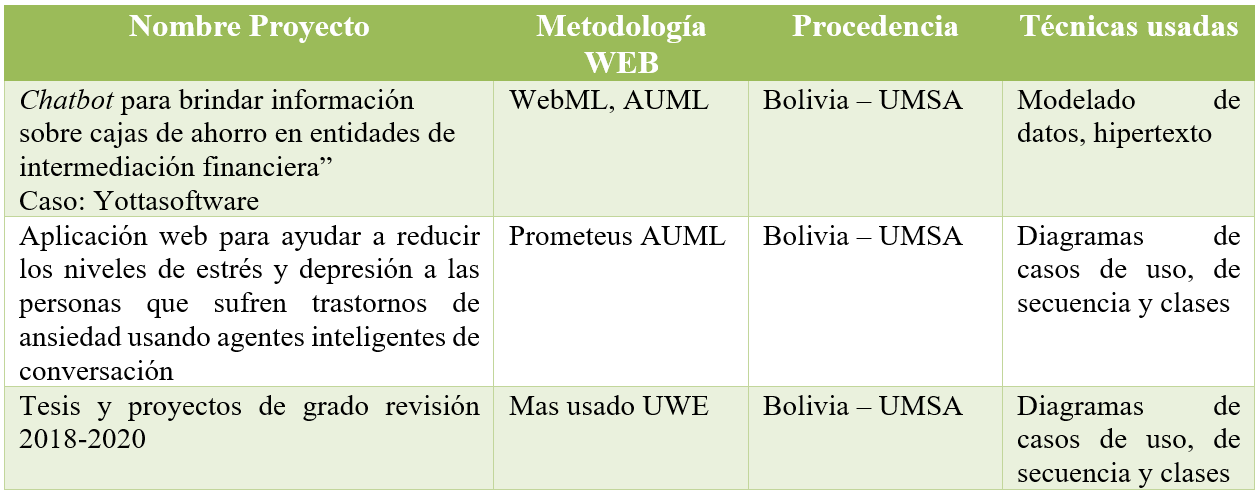
\includegraphics[width=1\textwidth]{tabla1_1}
\caption{Tabla comparativa de aplicaciones Web desarrolladas en la carrera de Informática.} 
\label{tab:tabla1_1} 
\end{table}

En la tabla 1.1 se aprecia como las metodologías y las representaciones gráficas usadas son los diagramas de clases, navegacionales, de clase, de secuencia y diagramas de entidad relación, de este estudio se definen las metodologías que se apoyan en UML o AUML para el desarrollo de cada etapa. Según Rios et. al (2018) se deben considerar los conceptos descritos en la Tabla 1.2.

\begin{table}[!ht]
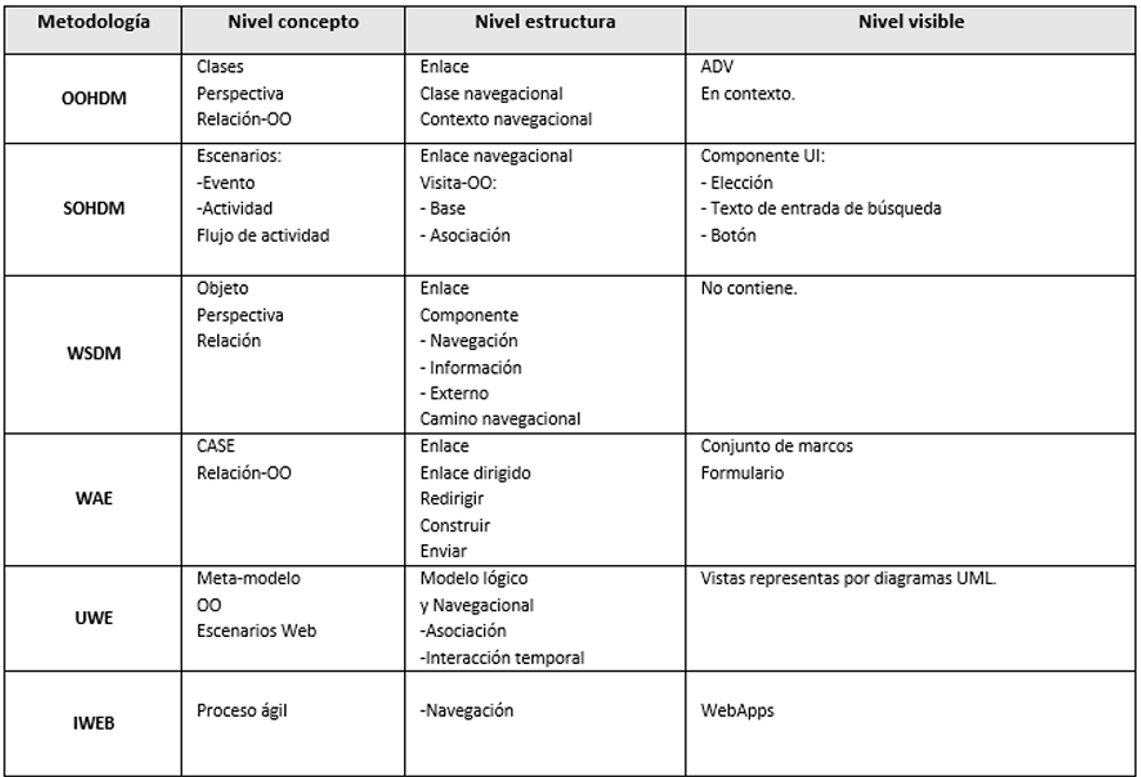
\includegraphics[width=1\textwidth]{tabla1_2}
\setcaptioncitation{(Rios et al., 2018)}
\caption{Comparación de conceptos de diseño de las metodologías de desarrollo Web}
\label{tab:tabla1_2} 
\end{table}

La tabla 1.2 representa el resultado de la comparativa de metodologías de desarrollo Web incluyendo UWE, WAE e IWEB, señalando como conclusión que las metodologías más usadas son OHDM y UWE, la primera definida por su fácil adaptabilidad para cualquier tipo de proyecto, respuesta inmediata ante problemas o errores que existen dentro del ciclo de vida, así como su fácil implementación y operatividad de cada proyecto, el segundo tiene un proceso iterativo e incremental que permite adaptar nuevos requerimientos y peticiones dentro el proyecto. 
\par
Por las características que ofrece la metodología UWE la figura 1.1 muestra los principales aspectos en los que se fundamenta son: 
\begin{itemize}
\item Uso de notación estándar UML lenguaje de modelado unificado.
\item Definición de métodos, que son los pasos para la construcción de los diferentes modelos.
\item Especificación de restricciones.
\end{itemize}

\begin{figure}[!ht]
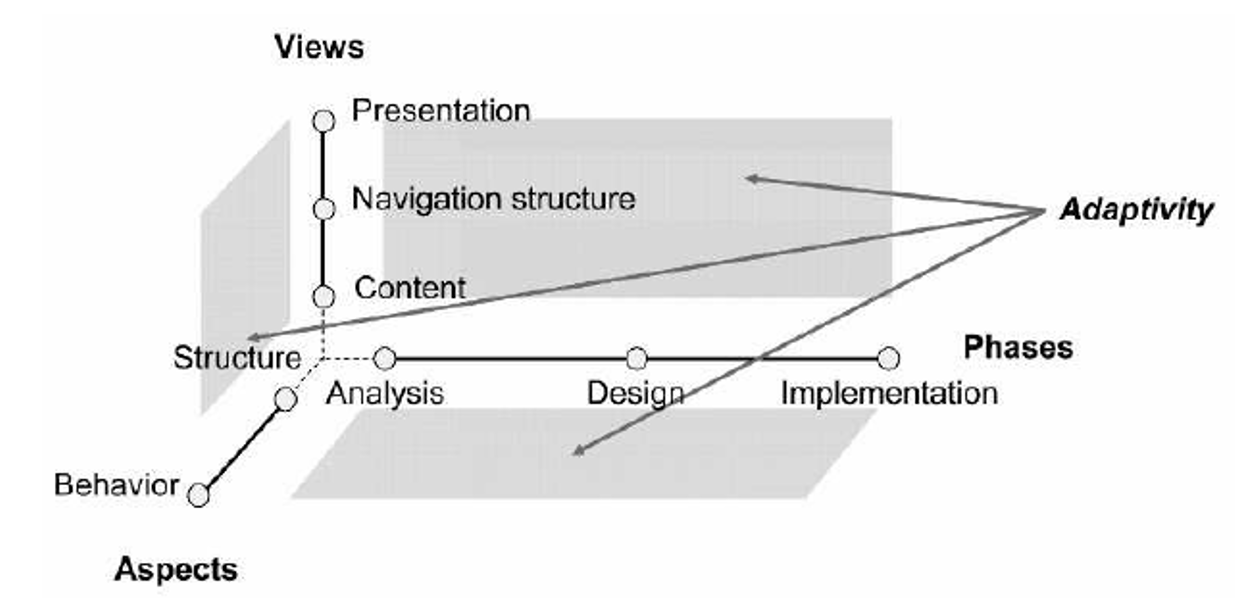
\includegraphics[width=1\textwidth]{figura1_1}
\setcaptioncitation{(Schwinger y Koch, 2006)}
\caption{Implementación gráfica de la metodología UWE basado en las fases, vistas y aspectos desarrollados}
\label{tab:figura1_1} 
\end{figure}

En las fases de la metodología se realizó el siguiente trabajo:
\begin{itemize}
\item \textbf{Análisis de requerimientos:} los requisitos funcionales se definían en tener un agente conversacional portable y de administración para el análisis, prueba y consultas realizadas al agente. 
\item \textbf{Diseño conceptual:} El modelo en el dominio de consultas de tramite generando actores para los casos de uso que tiene el agente con el público.
\item \textbf{Diseño navegacional:} Se realizaron bocetos o mockups en cada sprint relacionado al desarrollo de la aplicación y el árbol de rutas que tendrá incrementalmente, por cada historia de usuario desde los de alto riesgo a riesgo moderado.
\item \textbf{Diseño de Presentación:} Cada vista de la interfaz del usuario mediante los modelos desarrollados en la fase navegacional.
\end{itemize}

\subsection{METODOLOGÍA PARA EL DESARROLLO DE CHATBOTS}
La metodología IMADTC señala en su análisis de metodologías de desarrollo de \textit{chatbots} que existen metodologías que su foco principal se orienta a la solución propuesta a la fase de desarrollo del sistema que resuelva el problema, siendo una propuesta que se orienta su solución al análisis y captura de la información para un tratamiento de los problemas conceptuales como CDD desarrollo del manejo conversacional propuesto por el \textit{framework} RASA para el diseño de estructuras conversativas. La metodología IMDATC a orientado las fases para la construcción de las respuestas y contextos en el que se basará el agente conversacional de las cuales definidas a continuación se usó cada fase:

\begin{itemize}
\item \textbf{Contextualización del \textit{chatbot} en su dominio:} El agente conversacional se basa en objetivos definido como la pronta respuesta a una consulta no intentando ser un asistente de respuesta particularizada, operando en ese rol a un agente de preguntas frecuentes. Por la particularidad del proyecto no se podrá generar una interacción con los distintos sistemas web de las divisiones de la Universidad Mayor de San Andrés. 
\end{itemize}
Las fases que se ejecutarán cíclicamente se resolvieron de la siguiente manera:
\begin{itemize}
\item \textbf{Preparación de objetivos:} Por cada tramite se trató de responder de manera más general y sin tanto texto no necesario haciendo uso de las historias de usuario, basado en entrevistas y recopilación en base al uso del agente conversacional. 
\item \textbf{Diseño de flujo conversacional:} Con la información recabada en la anterior fase, se realiza un esquema representativo de conexión de las tareas encontradas como parte de la preparación de objetivos, usado como esqueleto generalizado de la lógica que debe seguir el \textit{bot} en un momento posterior de programación de los contextos.
\item \textbf{Prototipado:} En este punto con el flujo conversacional generalizado por cada tramite se tratará de generalizar las distintas salidas sobre cada pregunta en el \textit{framework} respuesta a cada pregunta. 
\item \textbf{Test de usuarios:} No basta con la obtención de estos flujos se debe mejorar con la prueba, esto sugerido en CDD, ya que su análisis define que se debe poner a prueba cíclicamente el \textit{chatbot}.
\end{itemize}

Se concluye que en este proyecto es necesaria la combinación de ambas metodologías separadas una de otra de la fase de implementación de la interfaz y el sistema web; luego desarrollando incrementalmente las estructuras conversacionales probables generalizadas por la continua mejora en fase de pruebas previas a lanzamiento. 


\chapter{MARCO TEÓRICO}

En este capítulo se desarrollan conceptos y teorías con respecto al conocimiento tanto en el desarrollo e implementación de una aplicación web, las bases fundamentales para el desarrollo de un agente de conversación y finalmente el análisis sobre el conjunto objetivo de trámites a tratar; todos estos conceptos representaron las bases académicas para el desarrollo de este trabajo siendo sintetizados para profundización posterior del lector.

\section{AGENTE VIRTUAL}
Según Kompella (2018): “La primera acuñación de \textit{chatterbot}, fue en 1994 por Michael Mauldin para definir sistemas conversacionales que intentan pasar el test de Turing, ELIZA creado en 1996 por Joseph Weizenbaum es conocida por ser el primer sistema conversacional en pasar  este Test parcialmente, el modelo de ELIZA entendía la entrada del usuario y trataba de emparejar las palabras clave con respuestas predefinidas, su diseño era el de conversar a través de emparejamiento de patrones y sustituciones; dando la ilusión que el contexto de la conversación era entendido por ELIZA.”

\begin{itemize}
\item \textbf{Funcionamiento de ELIZA}.- Considerando la oración de entrada “\textit{I want to run away from my parents}”, ELIZA asigna un valor en peso a cada palabra en la oración, siendo de peso menor los pronombres y de más alto peso los verbos de acción, con el valor más alto la acción actual, esto permitía al programa saber exactamente como hacer el cambio en la oración y preguntar de forma de cuestionamiento por pregunta. Reconociendo la regla particular asociada con el verbo de acción, entonces respondía con la respuesta que más empareje con las palabras clave, ¿así daba una respuesta “\textit{What would getting to run away from your parents mean you?}”. ¡Si el sistema de emparejamiento de reglas no obtenía una respuesta ELIZA tenía respuestas que eran genéricas para cualquier tipo de contexto, como ‘Porfavor prosigue’ o ‘Tengo un lindo día!’. ELIZA fue muy popular daba el presentimiento a las personas de estar hablando con un terapista; lo contrario a lo que buscaba Weizenbaum que desarrolló a ELIZA para mostrar una conversación de manera superficial entre un humano y una máquina; el sistema basado en reglas no podía mantener conversaciones significativas con las personas, luego muchos diseños basados en reglas se inspiraron como PARRY y ALICE (Gaikwad, 2019).
\end{itemize}

PARRY creado en 1972 por el psiquiatra Kenneth Colby, trataba de simular el modelo conversacional de personas con paranoia y esquizofrenia. PARRY implementaba un modelo crudo de comportamiento de una persona con paranoia y esquizofrenia, este comportamiento se basaba en juicios y creencias sobre conceptualizaciones en reacciones de aceptación, rechazo o neutrales. Era más complejo y avanzado que ELIZA, con una estrategia conversacional más robusta. Puesto a prueba en el test de Turing de 1970. Psiquiatras experimentados analizaron una combinación de pacientes reales y computadores mostrando las respuestas de PARRY en teleprompters, debían identificar cuales respuestas eran del paciente y cuáles del programa, acertaron solo 48\% del tiempo (Gaikwad, 2019).

\begin{itemize}
\item \textbf{Funcionamiento de PARRY}. – Algunos de los trucos que realizaba además de los mencionados con ELIZA eran admitir ignorancia, cambiar tema de conversación e introducir pequeñas historias sobre la mafia en la conversación, dando respuestas como “No te entiendo”, “Hablemos de algo más” y “Se que la mafia controla la producción” (Pereira et al., 2018).
\end{itemize}


ALICE (\textit{Artificial Linguistic Internet Computer Entity}) es un \textit{chatbot} creado en 1995 por el Doctor Richard Wallace en AIMG (\textit{Artificial Intelligence Markup Language}), un dialecto XML para la creación de asistentes virtuales. Inspirado por ELIZA ganando el premio Loebner en enero de 2000. La primera implementación fue llamada \textit{Program A} que fue escrito en lenguaje establecido en conceptos de conjuntos de teoría y lógica matemática llamada SETL. En 1998 se reescribió en JAVA. El \textit{program B} fue implementado en 1999, cuando 300 desarrolladores de \textit{software} se reunieron para escribir a ALICE y AIML cambió gramáticamente para ser compatible totalmente con XML, y ganó el premio Loebner como \textit{program B} en 2000 (Gaikwad, 2019).

Jabberwacky es un \textit{chatbot} creado por Rollo Carpenter, un programador británico, pensado para ser un \textit{bot} conversacional que imitara la interacción humana natural para propósitos de entretenimiento. Fue uno de los primeros intentos de \textit{chatbots} que implementando AI simulaba conversaciones humanas significativas. Ganando el premio Loebner en 2005 y 2006, una competición anual de test de \textit{chatbots}. Jabberwacky era capaz de aprender continuamente durante la conversación, los desarrolladores declararon que Jabberwacky no es implementado usando ningún modelo de vida artificial (sin redes neuronales o emparejamiento de patrones \textit{fuzzy}) y es basado puramente en algoritmos basados en heurística, no tenía ninguna regla codificada, en cambio se basa en la retroalimentación, almacenando las entradas de los usuarios y determinando la respuesta más apropiada usando técnicas de emparejamiento de patrones contextuales. Puesto línea desde 1997, Jabberwacky también fue re escrito en nuevos lenguajes (Gaikwad, 2019).

\subsection{AGENTES VIRTUALES COMERCIALES}
SmarterChild fue el primer chatbot comercial en tener una adopción dispersa. Lanzado en 2001 por ActiveBuddy como un servicio web integrado para el Mensajero Instantáneo de AOL. ¿daba respuestas a preguntas basados en hechos como “Cuál es la capital de Italia?” o “Quien ganó el juego de los \textit{lakers} la noche pasada?”. Antes de su cierre en 2007 gozaba de grabaciones en crecimiento y compromiso del usuario como un \textit{chatbot} usado por miles de personas todos los días. IBM Watson fue desarrollado en 2006 específicamente para competir con los ganadores del juego de Jeopardy. Watson ganó la competición en 2011, desde entonces; IBM Watson ofrece servicios para construir \textit{chatbots} para varios dominios los cuales pueden procesar grandes cantidades de datos. IBM lo llama “Computación Cognitiva”, aclamado por usar técnicas humanas para entender los datos y razonar. La salida de Siri en 2010 como un asistente virtual inteligente pavimento la forma para que otros asistentes virtuales como Google Now (2012), Cortana (2015) y Alexa (2015). \par
Todos estos asistentes ayudan a responder preguntas basadas en la web y acceso de ayuda en dispositivos móviles fácilmente. Recientemente, han mejorado sus capacidades como búsqueda basada en imágenes. Ya que todas esas tecnologías son comerciales, los detalles de implementación no se encuentran disponibles.

\section{TIPOS DE MODELOS PARA AGENTES VIRTUALES}
Según Lane (2019) “Los asistentes virtuales han recorrido un largo camino desde los días de ELIZA. La tecnología de coincidencia de patrones se ha generalizado y perfeccionado a lo largo de las décadas. Y se han desarrollado enfoques completamente nuevos para complementar la coincidencia de patrones. En la literatura reciente, los asistentes virtuales a menudo se denominan sistemas de diálogo, quizás debido a esta mayor sofisticación. Hacer coincidir patrones en el texto y completar plantillas de respuestas enlatadas con información extraída con esos patrones es solo uno de los cuatro enfoques modernos para crear asistentes virtuales:”

\begin{itemize}
\item Coincidencia de patrones: coincidencia de patrones y plantillas de respuesta (respuestas predefinidas o enlatadas).
\item \textit{Grounding}: gráficos de conocimiento lógico e inferencia sobre esos gráficos.
\item Búsqueda: Recuperación de texto por su denominación en ingles \textit{retrieval-based}.
\item Generativo: estadísticas y aprendizaje automático.
\end{itemize}

Siendo los de búsqueda y los de generación de texto asistentes virtuales de auto aprendizaje, y los de coincidencia de patrones y \textit{grounding } los asistentes virtuales basados en reglas.
\par
Según Bhaskar (2021): “La fundación básica de asistentes virtuales se basa en la mejor respuesta de cualquier pregunta que reciba. La mejor respuesta como responder las preguntas de usuario, proveer información relevante al usuario preguntar consultas siguiendo contexto. El diagrama siguiente es un mapa conceptual del desarrollo de asistente virtual basado en aprendizaje profundo:”

\subsection{ASISTENTES BASADOS EN RECUPERACIÓN DE TEXTO}
Modelos basados en obtención o recuperación de texto, han existido tradicionalmente como sistemas basados en reglas, teniendo un repositorio ajustado de respuestas mapeadas a preguntas. Alguno de los sistemas más sofisticados almacena contexto de la conversación, generando múltiples respuestas basados en contexto, evaluando cada respuesta y mostrando la que tiene mayor puntaje. Los sistemas basados en obtención ahora con técnicas de aprendizaje profundo para obtener respuestas más precisas., por tanto, obteniendo más contexto de la conversación y producir una respuesta sobre un sistema basado en obtención. Estas estrategias proveen mucha más precisión como control sobre el asistente virtual (Bhagwat, 2018).\par
Estos tipos de modelos dan respuestas basados en un repositorio de respuestas predefinidos. Se basan en la entrada y el contexto del usuario, una cierta heurística se define para seleccionar la respuesta apropiada. La heurística podría ser tan simple como un emparejamiento basado en reglas, o tan compleja como un ensamble de clasificadores de \textit{Machine Learning}. Aquí ningún texto nuevo es generado, en su lugar solo retorna la respuesta más probable basado en las respuestas ya conocidas. Debido a esto no son capaces de manejar en datos nunca vistos. Como no generan nuevas respuestas no producen errores gramaticales (Gaikwad, 2019). 

\begin{figure}[!ht]
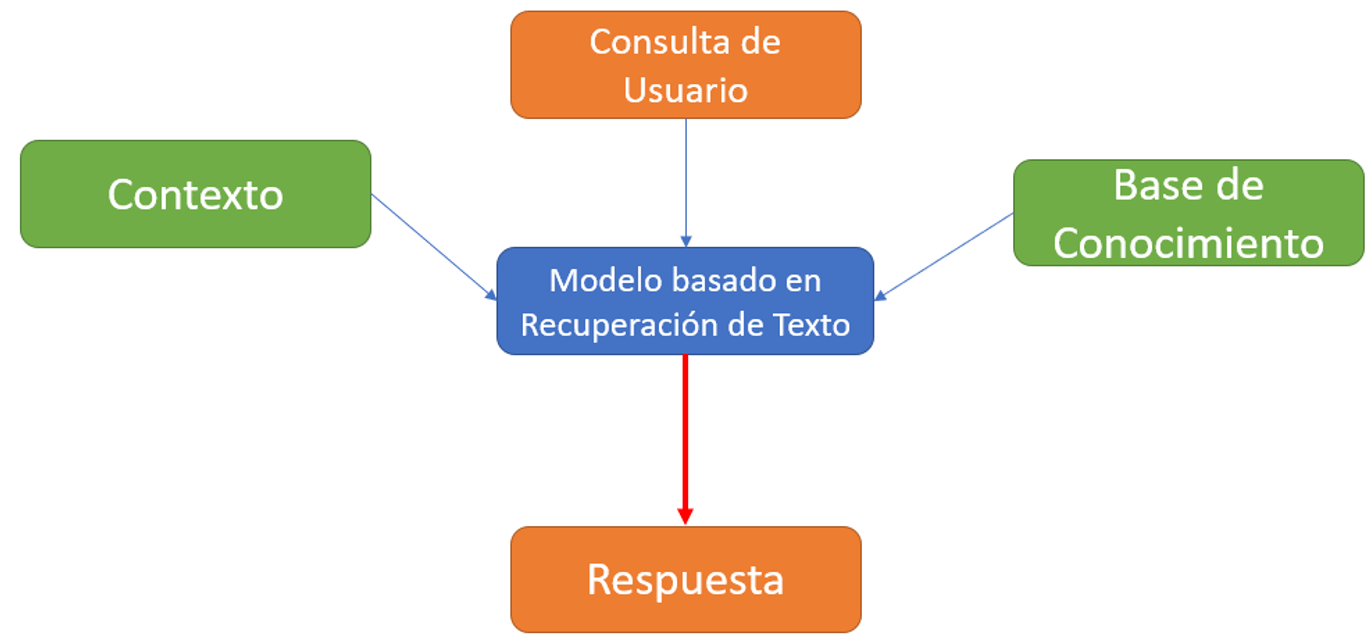
\includegraphics[width=1\textwidth]{figura2_1}
\caption{Modelo basado en Recuperación de Texto}
\label{tab:figura2_1} 
\end{figure}

La figura 2.1 muestra como un asistente virtual basado en búsquedas puede usar un registro de conversaciones pasadas para encontrar ejemplos de declaraciones similares a las que acaba de decir el compañero de conversación del \textit{bot}. Para facilitar esta búsqueda, el corpus de diálogo debe organizarse en pares declaración y respuesta. Si se responde a una respuesta, debería aparecer dos veces en su base de datos, una vez como la respuesta y luego otra vez como la declaración que provoca una respuesta. La columna de respuesta en la tabla de su base de datos se puede usar como base para la respuesta de su \textit{bot} a las declaraciones en la columna declaraciones o solicitud (Len, 2019).

\subsection{ASISTENTES BASADOS EN LA GENERACIÓN DE TEXTO}
Un asistente que usa el modelo generativo no utiliza ningún repositorio predefinido. Este tipo de \textit{chatbot} es más avanzado, porque aprende desde cero mediante un proceso llamado aprendizaje profundo. Los modelos generativos generalmente se basan en técnicas de traducción automática, pero en lugar de traducir de un idioma a otro, traducimos de una entrada a una salida. Otra forma de construir un sistema conversacional es usar técnicas de generación de lenguaje (Bhashkar, 2021).\par 
Los modelos de generación no usan respuestas predefinidas, en su lugar ellos crean nuevas respuestas y generan nuevo texto. Los modelos basados en generación toman inspiración de técnicas de máquinas de traducción, pero en lugar de traducir, aprenden de las respuestas de entrada y salida del usuario de la misma forma de traducciones de entrada y salida. Estos modelos tienden a ser difíciles de entrenar debido a las grandes cantidades de datos de entrenamiento requeridos y tienden a cometer errores gramaticales. (Gaikwad, 2019)

\begin{itemize}
\item \textbf{Modelos de secuencia a secuencia (Seq2Seq)}: Estos modelos de la secuencia entrenados para generar respuestas basadas en sus secuencias de entrada.
\item \textbf{Máquinas de Boltzmann (RBM)}: Cadenas de Markov entrenadas para minimizar una función de ‘energía’.
\item \textbf{Redes adversarias generativas}: Modelos estadísticos entrenados para engañar a un ‘juez’ de una buena conversación.
\end{itemize}

\subsection{VENTAJAS Y DESVENTAJAS DE LOS MODELOS DE RECUPERACIÓN Y GENERATIVOS}

Según Len (2019) existen muchas ventajas y desventajas al escoger cada aproximación para la resolución del problema de preguntas y respuestas; listados en la tabla 2.1.

\begin{table}[!ht]
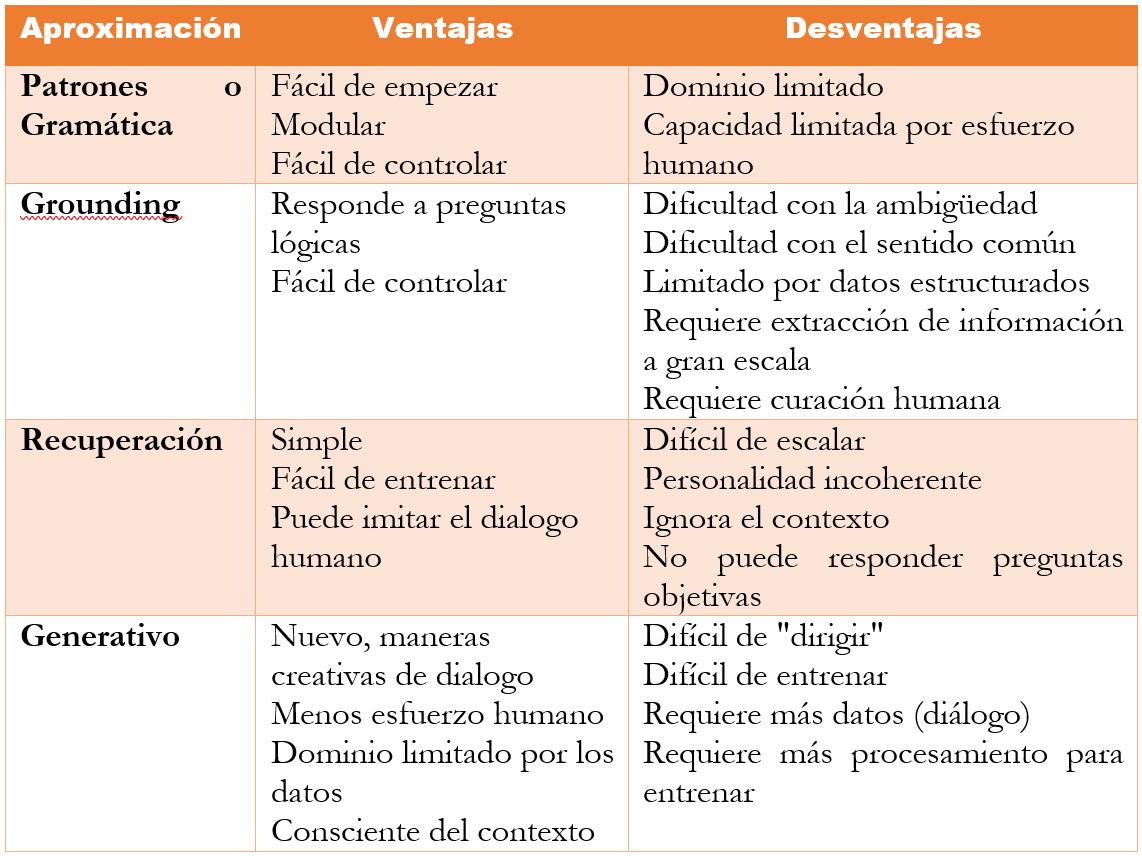
\includegraphics[width=1\textwidth]{tabla2_1}
\caption{Ventajas y Desventajas de los modelos para desarrollar asistentes virtuales}
\label{tab:tabla2_1} 
\end{table}

\section{COMPONENTES DE UN CHATBOT}
En palabras de Bhashkar (2021): “El \textit{chatbot} necesita ser capaz de entender las intenciones del mensaje del usuario, determinar qué tipo de mensaje de respuesta debe dar seguir la conversación, responder directamente y demás situaciones que se presentan en la particularidad de la utilidad del asistente virtual. Algunos de los modelos pueden usar meta información adicional de los datos, tales como id’s, géneros o emociones.”
\par
Según Raj (2018) “Hay tres pasos que uno debe seguir antes de construir un asistente virtual para pregunta y respuesta” 

\begin{enumerate}[label=(\alph*)]
\item Piense en todos los escenarios o tareas que desea que su asistente virtual pueda realizar y recopile todas las preguntas relacionadas en diferentes formularios que se pueden solicitar para realizar esas tareas. Cada tarea que desee que realice su asistente virtual definirá una intención, Cuando un usuario interactúa con un asistente virtual, ¿cuál es su intención de usar el \textit{chatbot}? Por ejemplo, cuando un usuario dice: "Reserva una entrada para el cine" a un \textit{chatbot}, nosotros, como humanos, podemos entender que el usuario quiere reservar una entrada para el cine. Esta es la intención de un \textit{bot}. 
\item Cada pregunta que enumere o intención se puede representar de varias maneras. Depende de cómo lo exprese el usuario. Por ejemplo: Alexa, apaga la luz. Alexa, ¿podrías apagar la luz? ¿Puedes por favor apagar la luz? Un usuario puede usar cualquiera de estas oraciones para indicarle al \textit{bot} que apague la luz. Todos estos tienen la misma intención de apagar la luz, pero se les pregunta en diferentes formas.  
\item Escriba toda su lógica para mantener al usuario vinculado al flujo que ha elegido después de reconocer la intención del usuario. Por ejemplo, suponga que está creando un \textit{bot} para programar una cita con el médico. Luego, le pide a su usuario que proporcione un número de teléfono, un nombre y un especialista, y luego le muestra los espacios y luego lo reserva.
\end{enumerate}


\section{COMO TRABAJA UN SISTEMA DE CONVERSACIÓN}

Según Bhashkar (2021): 'un asistente virtual se divide en sistemas que se dedican a una tarea en específico que al unirlos nos da una entrada que es la pregunta del usuario y una salida que es la respuesta que se refinó, condicionó y se calculó para que sea una respuesta a la pregunta con cierto grado de confiabilidad'

\begin{figure}[H]
\begin{center}
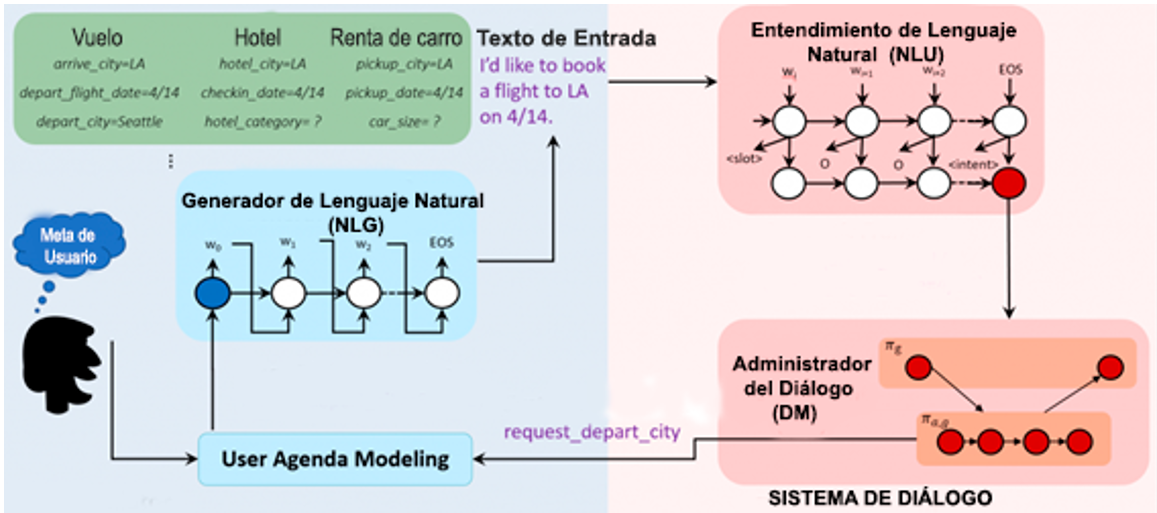
\includegraphics[width=0.7\textwidth]{figura2_2}
\setcaptioncitation{(Microsoft, 2016)}
\caption{Sistema de Dialogo de finalización de tareas compuestas}
\label{tab:figura2_2}
\end{center}
\end{figure}

La figura 2.2 muestra las distintas fases que pasa una interacción con un agente virtual, a continuación se describen las dos partes fundamentales que tiene un agente: 

\begin{enumerate}[label=(\alph*)]
\item \textbf{Entendimiento del lenguaje natural}. - La unidad NLU por sus siglas en inglés, es responsable de transformar el enunciado del usuario en un marco semántico predefinido de acuerdo con las convenciones del sistema, es decir, en un formato comprensible para el sistema. Esto incluye una tarea de llenado de ranuras y detección de intenciones. Como podemos ver, las intenciones y los espacios definen la naturaleza de dominio cerrado del asistente virtual (Bashkar, 2021).

\item \textbf{Generador del lenguaje natural}.- La unidad NLG por sus siglas en inglés es el proceso de generar texto de una representación significativa. Puede tomarse como el reverso de la comprensión del lenguaje natural. Los sistemas NLG proporcionan un papel fundamental para el resumen de texto, la traducción automática y los sistemas de diálogo. En NLG, la respuesta del sistema como un marco semántico, se mapea de nuevo a una oración de lenguaje natural, comprensible para el usuario final. El componente NLG puede estar basado en reglas o en modelos, en algunos escenarios puede ser un modelo híbrido, es decir, una combinación de ambos. El NLG basado en reglas genera algunas oraciones de plantilla predefinidas para un marco semántico dado, por lo que son muy limitadas y no tienen ningún poder de generalización. Si bien se han desarrollado varios sistemas de generación basados en reglas de propósito general, a menudo son bastante difíciles de adaptar a aplicaciones pequeñas y orientadas a tareas debido a su generalidad. Los sistemas NLG basados en aprendizaje automático (entrenables) son más comunes en los sistemas de diálogo actuales (Bashkar, 2021).

\item \textbf{Administrador de Dialogo}.- DM por sus siglas en inglés puede ser conectado a alguna base de conocimiento externa (KB) o una base de datos (DB), tales son los que producen respuestas significativas predefinidas. El administrador del diálogo puede ser una máquina de estado finito, un cambio de oración con intenciones que dan diferentes respuestas aleatorias, basado en metas y basado en confianza donde se fía de la unidad NLU (Bashkar, 2021).

\end{enumerate}



Después de definir las características que debe tener un agente conversacional, se tomó en cuenta también los servicios más actuales de implementación de un agente virtual, la siguiente sección engloba las distintas herramientas usadas para desarrollar un agente basado en recuperación. 

\section{HERRAMIENTAS DE ANÁLISIS DE LENGUAJE NATURAL}

Los \textit{softwares} de \textit{chatbots} han incrementado su uso en el dominio de la Ingeniería de \textit{Software} desde que permiten a los usuarios interactuar con plataformas usando lenguaje natural, automatizando las tareas tediosas y evitando el tiempo y esfuerzo. Como consecuencia de la diversidad de NLU ampliamente utilizadas, los desarrolladores se enfrentan a la selección de la mejor NLU para su dominio particular. Esta es una tarea no trivial y ha sido discutido en gran medida en el trabajo anterior especialmente desde NLU varían en rendimiento en diferentes contextos. (Abdellatif A., et.al., 2021)
\par
Según (Astruga, J., 2022): “El método seguido para realizar el análisis a la hora de escoger una alternativa tecnológica al uso de \textit{chatbots} consiste en seleccionar (de acuerdo a criterios relacionados con los problemas de carácter tecnológico especificados como relevantes para la problemática, aquellas alternativas que sean adecuadas para el trabajo a realizar. Los criterios utilizados a la hora de analizar las tecnologías son:”
\begin{itemize}
\item \textbf{Disponibilidad}.- Licencia bajo la que opera el sistema y precios de concesión de licencia para uso, desarrollo y comercialización de derivados del producto. 
\item \textbf{Definición del modelo del agente en el sistema}.- Qué elementos constituye una definición del agente, si dispone de los elementos típicos en un \textit{chatbot}, es decir, \textit{intents}, \textit{entities} y contextos del diálogo y cómo es su uso en el sistema.
\item \textbf{Cómo se realiza el procesamiento del lenguaje natural en el sistema}.- Que se necesita para que el sistema lleve a cabo el procesamiento del lenguaje natural en el sistema y cómo se mejora la identificación de secciones clave dentro de una oración como el \textit{intent} o las \textit{entities}. 
\item \textbf{Idiomas del sistema}.- En que idiomas está disponible el sistema para llevar a cabo el procesamiento del lenguaje natural, si se requiere entrenar el sistema para que sea capaz de reconocer oraciones en español e ingles o si requiere software adicional.
\item \textbf{Interfaces del sistema}.- interfaces de interacción con el sistema. Tanto interacción a la hora de realizar la programación y creación del agente conversacional como a la hora de interactuar con el sistema a partir de otros sistemas clientes.
\item \textbf{Tratamiento de datos aportados por los usuarios}.- Cómo es el tratamiento que se hace de los datos de los usuarios al hacer este uso del sistema, se necesita saber si se mantiene la confidencialidad de los datos aportados, si estos datos son usados para la mejora del sistema o si estos datos son cedidos para uso de terceros.

\end{itemize}


Dado lo descrito se procede a considerar dos de las tres alternativas más utilizadas para el desarrollo de un \textit{chatbot}, primero como una plataforma de NLU o entendimiento del lenguaje natural se hará uso de Dialogflow por conveniencia práctica, no se considerará LUIS que es la implementación del entorno Azure de Microsoft para un agente conversacional, y el \textit{framework} de aprendizaje automático de uso libre Rasa, como una alternativa a Dialogflow y LUIS de uso libre que no contiene límites en su uso, luego se hará un análisis respectivo de ambos servicios que usan técnicas de lenguaje natural para encontrar la intención del mensaje propuesto por el usuario. 

\subsection{DIALOGFLOW}
Dialogflow es una plataforma con comprensión del lenguaje natural que facilita el diseño de una interfaz de usuario de conversación y su integración para dispositivos móviles, aplicaciones web, dispositivos, \textit{bots}, sistemas de respuesta de voz interactiva y más.  Dialogflow puede analizar múltiples tipos de entradas de tus clientes, incluidas entradas de texto o audio como las de un teléfono o una grabación de voz. También puede responder a tus clientes de varias maneras, ya sea a través de texto o con voz sintética. Se usó la versión gratuita denominada Dialogflow ES y su implementación con el uso de su API REST disponible para NodeJS. 
\par 
Las interfaces informáticas tradicionales requieren entradas predecibles y estructuradas para funcionar de manera correcta, lo que hace que el uso de estas interfaces no sea natural y, a veces, sea difícil. Si los usuarios finales no pueden comprender estas entradas estructuradas con facilidad, se les dificulta decidir qué hacer. Lo ideal es que sean interfaces que puedan inferir lo que desean los usuarios finales, según el lenguaje natural que usen. Por ejemplo, considera una solicitud de usuario sencilla, como: “¿Cuál es el pronóstico para hoy?” Otros usuarios finales también pueden preguntar lo siguiente:
\begin{itemize}
\item ¿Cuál es el clima en este momento?
\item ¿Qué temperatura hará mañana en San Francisco?
\item ¿Cómo estará el clima el 21?
\end{itemize}
Incluso con estas preguntas sencillas, puedes ver que las experiencias de conversación son difíciles de implementar. Interpretar y procesar el lenguaje natural requiere un analizador de lenguaje muy sólido.
Un agente de Dialogflow es un agente virtual que maneja conversaciones con los usuarios finales. Es un módulo de comprensión del lenguaje natural que entiende los matices del lenguaje humano. Dialogflow traduce el texto o el audio del usuario final durante una conversación a datos estructurados que tus apps y servicios pueden comprender. Un agente de Dialogflow se crea y diseña a fin de manejar los tipos de conversaciones requeridas para tu sistema.

\subsection{INTENCIONES}

Se trata de clasificar la intención del usuario para un intercambio conversacional, la combinación de \textit{intents} puede manejar una conversación completa, la conversación de entrada del usuario se denomina expresión de usuario final, el agente hace coincidir la expresión del usuario final con el mejor \textit{intent} en el agente, realizando una clasificación en la intención del mensaje.
\par
Como se muestra en la figura 2.3 la consulta “¿Cuál es el pronóstico?” se hará coincidir esa expresión con el \textit{intent} del pronóstico. También se puede definir un \textit{intent} con el fin de extraer información útil de la expresión del usuario, como una hora o ubicación para el pronóstico del tiempo deseado, estos datos extraídos son importantes a fin de que tu sistema realice una consulta cobre el clima para el usuario final. 

\begin{figure}[!h]
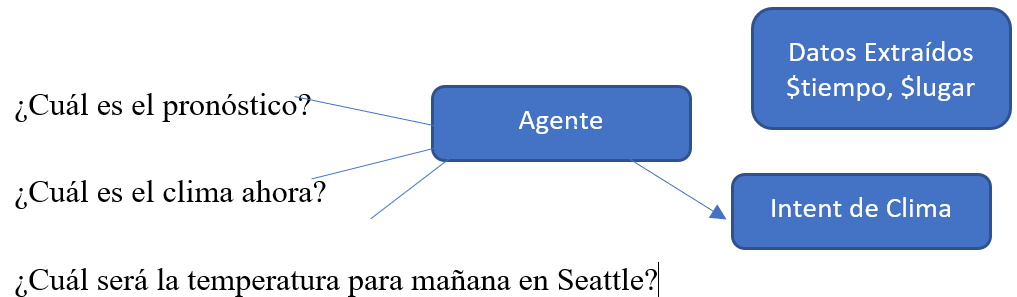
\includegraphics[width=1\textwidth]{figura2_3}
\caption{Clasificación de intención y parámetros}
\label{tab:figura2_3} 
\end{figure}


Cada intención básica contiene los siguientes elementos:
\begin{itemize}
\item \textbf{Frases de Entrenamiento}.- Frases de ejemplo de algo que podrían decir los usuarios finales, cuando una expresión se parece a alguna de estas frases, se hará una coincidencia con el \textbf{intent}, no es necesario definir todos los ejemplos posibles, ya que se expande la lista con aprendizaje automático usado en Dialogflow.
\item \textbf{Acción}.- Se puede definir una acción para cada \textbf{intent}; cuando este coincide el agente de Dialogflow proporciona la acción al sistema, y se puede usar la acción definida en el sistema. 
\item \textbf{Parámetros}.- Dialogflow proporciona los valores extraídos de la expresión del usuario final como parámetros, cada parámetro tiene un tipo, llamado entidad, que dicta cómo se extraen los datos. A diferencia de la entrada sin procesar del usuario final, los parámetros son datos estructurados que se pueden usar fácilmente para realizar alguna lógica o generar respuestas.
\item \textbf{Respuestas}.- Las respuestas proporcionan al usuario la información que se necesite para finalizar la conversación. 
\end{itemize}


\subsection{ENTIDADES}
Cada parámetro de \textit{intent} tiene un tipo, denominado tipo de entidad, determina de forma exacta cómo se extraen los datos de una expresión de usuario final, Dialogflow proporciona entidades del sistema que coinciden con fechas, horas, colores, direcciones de correo electrónico, etcétera. También se pueden crear entidades personalizadas propias para detectar coincidencias de datos personalizados, como por ejemplo una entidad vegetal que coincida con los tipos de vegetales disponibles para la compra con un agente de supermercado. 

\subsection{CONTEXTO}
Los contextos son igual a los contextos de lenguaje natural. Si una persona dice “es de color naranja”, necesita contexto para saber qué es de ese color, para que Dialogflow maneje una expresión de usuario final como esa, debe proporcionarse un contexto con el fin de que coincida de forma correcta con un \textit{intent}. Mediante los contextos, se puede controlar el flujo de una conversación. Se puede establecer contextos de entrada y salida, que se identifican mediante nombres de \textit{strings}, cuando coincide un \textit{intent}, se activan los contextos de salida configurados para este; mientras existan contextos activos, es más probable que Dialogflow coincida con intents configurados con contextos de entrada que correspondan a los contextos activos en ese momento.

\par
En la figura 2.4, primero el agente hace coincidir con la intención de revisar información el cual tiene un contexto de salida de revisar, por lo que ese contexto se activa, el agente le solicita al usuario final el tipo de información que desea obtener sobre su cuenta corriente, cuando el usuario responde “mi saldo”, Dialogflow hace coincidir esta expresión del usuario final con la intención de revisar balance, este tendrá un contexto de entrada revisar, que debe estar activo para que coincida con este, también puede existir una intención de guardar balance similar para que coincida con la misma expresión del usuario final cuando un contexto de guardar este activo.


\begin{figure}[H]
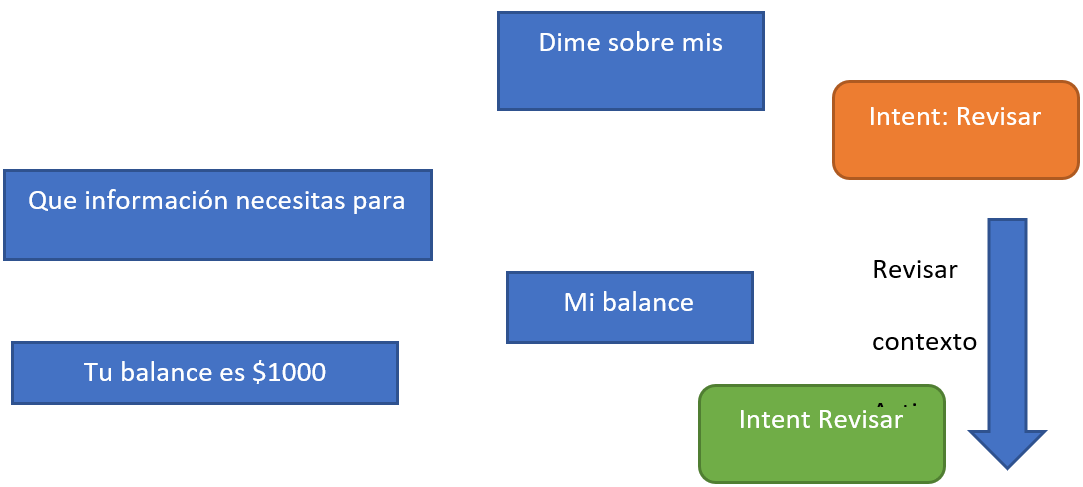
\includegraphics[width=1\textwidth]{figura2_4}
\caption{Flujo conversacional con el uso de contextos de entrada y salida}
\label{tab:figura2_4} 
\end{figure}

\subsection{RASA}
Mantener una conversación requiere dos habilidades básicas: comprender lo que se dice y responder de acuerdo con eso. Rasa es un \textit{framework} de inteligencia artificial de código abierto  que proporciona las herramientas necesarias para crear asistentes de \textit{chat} contextualizados. Rasa Open Source incluye los siguientes módulos:

\begin{itemize}
\item \textbf{Rasa NLU}.- Es la unidad de procesamiento del lenguaje natural para comprender el lenguaje de entrada. Proporciona las herramientas para la clasificación de intenciones (de lo que habla el usuario) y la extracción de entidades (cuál es la información clave).
\item \textbf{Entidades}.- Corresponden a las entidades de primer nivel que queremos manejar en nuestro agente. 
\item \textbf{Intenciones}.- acciones que corresponden a la lógica de negocio (entrada de datos por parte del usuario) y que va a realizar nuestro agente.
\end{itemize}

\subsection{RASA CORE}
Rasa Core es el motor de diálogo de Rasa que se encarga de decidir el próximo curso de acción en función de la información de Rasa NLU. En lugar de usar una condición simple si o no, utiliza el aprendizaje automático para aprender de conversaciones anteriores y actuar en función de ese conocimiento.
\par
Rasa funciona como una abstracción sobre las bibliotecas NLP de nivel más bajo como SpaCy, nltk, sklearn, etc., y proporciona un marco que combina las herramientas necesarias para crear asistentes de conversación contextualizados que funcionen plenamente. El módulo Rasa NLU convierte el lenguaje natural en datos estructurados. Este módulo puede hacer dos cosas: clasificación de intenciones y extracción de entidades. La clasificación por intención es un proceso de dos pasos. 
\par
Primero, se provee a un modelo NLU con datos de entrenamiento etiquetados que incluyen una lista de intenciones conocidas y los textos de ejemplo correspondientes. Como segundo paso se entrena el modelo, el modelo puede clasificar un nuevo texto de entrada en una de las intenciones predefinidas. La extracción de entidades es el proceso de identificar y extraer piezas clave de información en un texto dado. Una entidad puede ser cosas como hora, lugar, nombre de una persona, entre otros datos importantes para el desarrollador. 
\par 
El módulo Rasa Core toma la salida de Rasa NLU (intención y entidades) y los alimenta a los modelos de aprendizaje automático y genera una respuesta. También es responsable de controlar el flujo de la conversación. 

\par

Una vez definidas las dos herramientas que servirán tanto de implementación como guía en la construcción de circuitos de conversación, la siguiente sección continúa explorando el campo de las redes neuronales en el area de procesamiento del lenguaje. 


\section{PROCESAMIENTO DEL LENGUAJE NATURAL}

El procesamiento del lenguaje natural es un área de investigación en informática e inteligencia artificial relacionada con el procesamiento de lenguajes naturales como el inglés o el mandarín. Este procesamiento generalmente implica traducir el lenguaje natural en datos numéricos que una computadora puede usar para aprender sobre el mundo. Y esta comprensión del mundo a veces se usa para generar texto en lenguaje natural que refleja esa comprensión. Un sistema de procesamiento de lenguaje natural a menudo se denomina "\textit{pipeline}" porque generalmente involucra varias etapas de procesamiento donde el lenguaje natural fluye en un extremo y la salida procesada fluye hacia el otro (Len, 2019).
\par 
Lo interesante del proceso es que es difícil. Las máquinas con la capacidad de procesar algo natural no son naturales. Es como construir un edificio que puede hacer algo útil con diagramas arquitectónicos. Cuando el \textit{software} puede procesar lenguajes que no están diseñados para que las máquinas los entiendan, parece mágico, algo que pensamos que era una capacidad exclusivamente humana (Len, 2019).
\par 
Es un campo de la inteligencia artificial que permite a las computadoras analizar y entender el lenguaje humano, tenemos cientos de métodos como NLU \textit{Natural Language Understanding}, se debería saber que no hay nada artificial en AI, en esencia son algoritmos de aprendizaje profundo o automático escrito por personas, corriendo por debajo, aún no se ha alcanzado la etapa en donde las máquinas hayan alcanzado a analizar como los humanos para poder percibirse a sí mismas inteligencia, se debe escribir algoritmos y usar técnicas de NLP, que es considerado el cerebro de los chatbots que procesa los datos crudos, los afinan, limpian y los prepara para las acciones apropiadas (Raj, 2018).

\subsection{TOKENIZACIÓN}
La tokenización trata de segmentar un texto en \textit{tokens} es un tipo de segmentación de documento. La segmentación rompe el texto en pequeños partes o segmentos conteniendo la mayor información posible, sean párrafos, oraciones, frases o \textit{token} usualmente palabras. Un \textit{tokenizer} en el contexto de compiladores usado para compilar lenguajes de programación se llama \textit{scanner} o \textit{lexer}. El vocabulario conjunto de tokens se llama \textit{lexicon}. La manera más simple de tokenizar un texto es por el espacio entre palabras como delimitador. Ahora se puede crear un vector representación para cada palabra llamado “\textit{One hot vectors}”, una secuencia de estos vectores puede capturar el texto original en secuencias de vectores. Los vectores \textit{one hot} son súper dispersos y contienen solo un valor distinto de cero en cada vector de fila. Cada fila de la tabla es un vector de fila binario qué también se le llama vector único: todas menos una de las posiciones (columnas) en una fila son 0 o están en blanco. Solo una columna, o posición en el vector es distinta de cero. Lo importante es convertir una oración de palabras del lenguaje natural en una secuencia de números o vectores (Len, 2019).
\par 
Según Raj (2019): “La tokenización es uno de los conceptos simples pero básicos de NLP donde dividimos un texto en segmentos significativos. El método de división en cualquier lenguaje de programación que separa en una lista basado en los espacios por defecto es solo un método sin formato para dividir la oración en \textit{tokens} dado un separador. No tiene en cuenta ningún significado, mientras que la tokenización también intenta preservar el significado.”

\subsection{EXPRESIONES REGULARES}
El análisis y procesamiento de texto es un gran tema en sí mismo. A veces, las palabras juegan juntas de una manera que hace que sea extremadamente difícil para las máquinas entenderlas y entrenarlas. La expresión regular puede ser útil como respaldo para un modelo de aprendizaje automático. Tiene el poder de la coincidencia de patrones, lo que puede garantizar que los datos que se está procesando sean correctos o incorrectos. La mayoría de los primeros \textit{chatbots} dependían en gran medida de la coincidencia de patrones (Raj, 2019).

\subsection{N-GRAMS}
Los n-grams son secuencias que contienen n elementos pueden ser caracteres, silabas, palabras o símbolos, pero 2-gram ahora significa par de palabras, 3-gram tres palabras juntas como ‘Jhoan Sebastian Bach’ que en conjunto presenta un significado no como \textit{tokens} como ‘Jhoan’ o ‘Sebastian’ que separa un \textit{token} que compone más de una palabra que resulta significativo, cuando una secuencia de tokens se vectoriza en un vector pierde mucho del significado inherente al orden de esas palabras. Al ampliar el concepto de un \textit{token} para incluir \textit{tokens} de varias palabras, n-gramas, su tubería de NLP puede conservar gran parte del significado inherente al orden de las palabras en sus declaraciones, Se retiene un poco del contexto de una palabra cuando la vinculación a sus vecinos (Len, 2019).

\subsection{STOP WORDS}
Las palabras vacías son palabras comunes en cualquier idioma que ocurren con mucha frecuencia pero que contienen mucha menos información sustantiva sobre el significado de una frase. Ejemplos de algunas palabras vacías comunes incluyen, ‘en’, ‘el’, ‘etc’. Históricamente, las palabras vacías se han excluido de las canalizaciones de NLP para reducir el esfuerzo computacional para extraer información de un texto. Aunque las palabras en sí contienen poca información, las palabras vacías pueden proporcionar información relacional importante como parte de un n-gram (Len, 2019).
\par
Las palabras vacías son palabras de alta frecuencia como que a veces queremos filtrar de un documento antes de continuar con el procesamiento. Las palabras vacías suelen tener poco contenido léxico y no tienen mucho significado. Siempre puede definir sus propias palabras vacías si es necesario y anular la lista existente. Las palabras vacías son una parte muy importante de la limpieza del texto. Ayuda a la eliminación de datos sin sentido antes de que intentemos hacer un procesamiento real para dar sentido al texto (Raj, 2018).

\subsection{STEMMING}
Una técnica común de normalización del vocabulario es eliminar las pequeñas diferencias de significado de la pluralización o las terminaciones posesivas de las palabras, o incluso varias formas verbales. Esta normalización, que identifica una raíz común entre varias formas de una palabra, se denomina stemming. Por ejemplo, las palabras vivienda y casas comparten la misma raíz, casa. Un ser humano puede ver fácilmente que ‘casa’ y ‘casas’ son las formas singular y plural del mismo sustantivo. Sin embargo, necesita alguna forma de proporcionar esta información a la máquina. Uno de sus principales beneficios está en la compresión de la cantidad de palabras cuyos significados necesita realizar un seguimiento de su software o modelo de lenguaje. Reduce el tamaño de su vocabulario mientras limita la pérdida de información y significado, tanto como sea posible. En el aprendizaje automático, esto se conoce como reducción de dimensión. Eliminación de ‘correr’ a ‘corre’ devolviendo al caso base, pero existe una diferencia entre \textit{stemming} y lematización. (Len, 2019)

\subsection{LEMATIZACIÓN}
La lematización consiste en tener información sobre las conexiones entre los significados de varias palabras, es posible poder asociar varias palabras, incluso si su ortografía es bastante diferente. Esta normalización más extensa hasta la raíz semántica de una palabra, su lema, se denomina lematización. Usarlo puede hacer que su modelo sea más general, pero también puede hacer que su modelo sea menos preciso, porque tratará todas las variaciones ortográficas de una palabra raíz dada de la misma manera (Len, 2019).
La lematización está estrechamente relacionada con la lematización, pero la lematización es el proceso algorítmico de determinar el lema de una palabra en función de su significado previsto. Por ejemplo, en inglés, el verbo ‘caminar’ puede aparecer como ‘caminaste’, ‘anduviste’, ‘caminas’ o ’caminando’. La forma base, ‘caminar’, que uno podría buscar en un diccionario, se llama el lema de la palabra. (Raj, 2018)


\subsection{WORD EMBEDDING}
Gaikwad (2019) asegura que: “Ya que las computadoras son incapaces de entender el concepto de palabras, un mecanismo para representar texto es usar la entrada de proceso de lenguaje natural. Para una tarea NLP en aprendizaje profundo, usamos una capa de preprocesamiento en la arquitectura RNN llamada \textit{embedding layer}. El mecanismo para el mapeado de texto se llama \textit{word vector}, el cual envuelve representación de palabras u oraciones usando vectores de números reales. \textit{Neural word embedding} permite al contexto ser capturado en oraciones aprendiendo las semánticas de distribución de las palabras. \textit{Word embeddings} son usados para capturar el contexto y representar las relaciones entre palabras. Los modelos más populares para creación y aprendizaje Word2Vec y GloVe. Word2Vec toma un corpus grande de texto como entrada y crea un espacio de vector dimensional, usualmente de cientos de dimensiones. Cada palabra en el corpus es asignada a un vector espacio y posicionada así las palabras las cuales tienen similar contexto en el corpus están cercanas en proximidad”. 

\begin{figure}[H]
\begin{center}
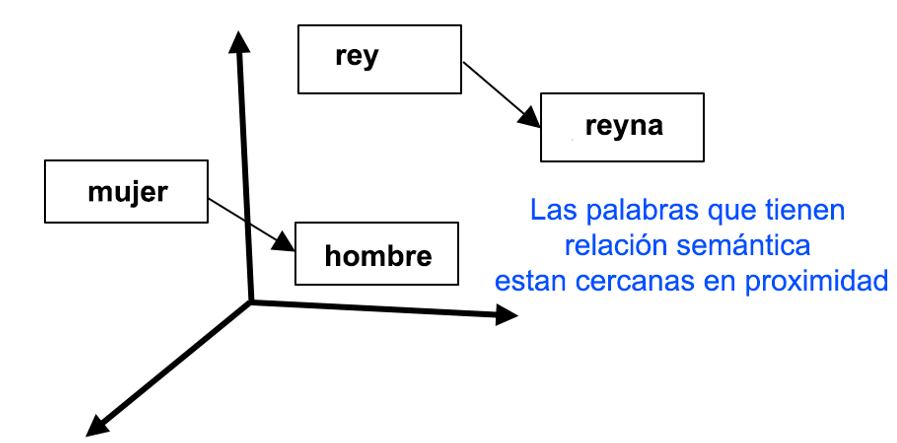
\includegraphics[width=0.8\textwidth]{figura2_5}
\setcaptioncitation{(Len, 2019)}
\caption{Relación semántica de Word2Vec}
\label{tab:figura2_5} 
\end{center}
\end{figure}

Como se muestra en la figura 2.5 Word2Vec pueden usar de dos modelos de arquitecturas para producir una representación distribuida de palabras: \textit{continuous bag-of-words} (CBOW) o \textit{skip-gram} continuo. En la arquitectura de \textit{continuos bag-of-words}, el modelo predice la palabra acutal de una ventana de \textit{surrounding context words}. El orden del contexto de palabras no influye en la predicción. En la arquitectura \textit{skip-gram} pesos cercanos de palabras de contexto son más pesadas que mas distantes palabras de contexto. Acorde a los autores CBOW es más rápido mientras que skip-gram es lento pero hace un mejor trabajo para palabras infrecuentes. Para preprocesado, un modelo Word2Vec pre entrenado es usado para crear vectores \textit{word embedding} para algún corpus (Bhagwat, 2019).

\subsection{REDES NEURONALES ARTIFICIALES}
Las redes neuronales artificiales presentan una estructura flexible inspirados por el principio de procesamiento de información en sistemas biológicos una red neuronal de un ser humano, consiste en representaciones matemáticas de unidades de procesamiento conectadas llamadas neuronas artificiales. Como sucede con la sinapsis en el cerebro cada conexión entre neuronas transmiten señales cuya fuerza puede ser amplificada o atenuada por un peso que es continuamente ajustado durante el proceso de aprendizaje forzando conexiones entre neuronas o debilitándola. 


\begin{figure}[H]
\begin{center}
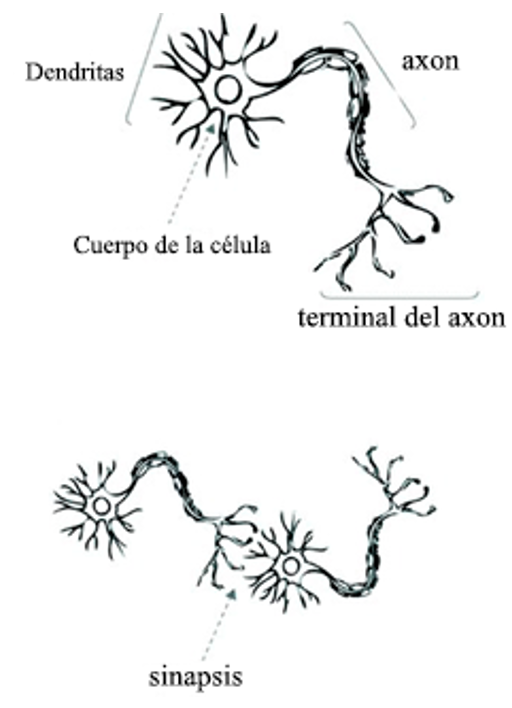
\includegraphics[width=0.3\textwidth]{figura2_6}
\setcaptioncitation{(MengZenzhu, 2020)}
\caption{Ejemplo gráfico de una neurona y redes neuronales}
\label{tab:figura2_6} 
\end{center}
\end{figure}



En la figura 2.6 se muestra como son las neuronas, se puede apreciar como cada señal es procesada por neuronas subsecuentes si se excede cierto umbral determinado por una función de activación, típicamente las neuronas se organizan en capas, una capa de entrada recibe datos de entrada sean analíticos, imágenes, sonido y una capa de salida produce el resultado final que se espera, la variabilidad de una red neuronal en capas y cantidad de neuronas dependen de la elección de propiedades como la taza de aprendizaje o la función de activación que constituyen hiper-parámetros de cada modelo que deben ser actualizados manualmente juzgados por una rutina de optimización (Goodfellow et al., 2017).

\subsection{REDES NEURONALES PROFUNDAS}
Foster (2018) indica que “Una red neuronal profunda es una red neuronal con múltiples capas ocultas para poder aprender representaciones de alto nivel en las entradas de datos no estructurados con cada capa contenida por múltiples unidades que se conectan con capas previas a través de un conjunto de pesos, y con capas apiladas las unidades de cada subsecuente pueden representar aspectos más sofisticados de la entrada, pero la magia está en encontrar un conjunto de pesos para cada capa que de resultado a predicciones más precisas”.

\begin{enumerate}[label=(\alph*)]
\item \textbf{Backpropagation}.- Durante el proceso de entrenamiento los datos pasan a través de la red neuronal y la salida se compara con la salida esperada, el error en la predicción se propaga por toda la red del final al principio ajustando el conjunto de pesos cada uno en dirección para que se mejore la predicción significativamente es el proceso denominado backpropagation que gradualmente cada unidad sea más hábil en identificar una característica particular que ayude a predecir eficientemente a toda la red  (Goodfellow et al., 2017).
\item \textbf{Función de Activación}.- La función de activación es crítica para asegurarse que la red neuronal es capaz de aprender funciones complejas y no solo una salida que es una combinación lineal de la primera entrada, existe varias funciones de activación como ReLU, sigmoidal, softmax que son las más usadas. La salida de una unidad en la red es la suma de los pesos de la entrada recibida por las capas previas que pasa por una función de activación no lineal antes de ser enviada a la capa siguiente (Foster, 2018).
\item \textbf{ReLU y LeakyReLU}.- Unidad lineal rectificada o ReLU es una función de activación o umbral que devuelve cero si una entrada es negativa, caso contrario iguala la entrada, existe también leakyReLU que en lugar de devolver cero retorna una cantidad menor al número negativo, la figura 2.7 muestra las dos funciones de activación.

\begin{figure}[H]
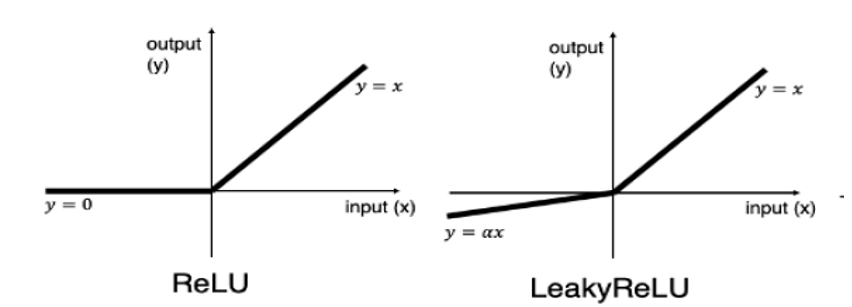
\includegraphics[width=0.8\textwidth]{figura2_7}
\setcaptioncitation{(Foster, 2018)}
\caption{Funciones de activación \textit{ReLU y LeakyReLU} }
\label{tab:figura2_7} 
\end{figure}

\item \textbf{Función de perdida}.- Se usa una función de perdida para comparar la salida con la muestra de salida real, retorna un valor por cada observación (más grande es el valor, peor es el rendimiento de la red neuronal para cada observación) las más comunes son. Error de la media cuadrática o \textit{mean square error}, entropía cruzada categórica y entropía categórica binaria, como escoger entre estas dependerá de la optimización que se quiera en la red Foster (2018).

\item \textbf{Optimizador} El optimizador es el algoritmo que será usado para actualizar los pesos en la red neuronal basado en la gradiente de la función de perdida una de las más comunes ADAM es una buena opción de optimizador se debe tener en cuenta el radio de aprendizaje mientras más alto, más bruscos son los cambios en los pesos de las neuronas en cada entrenamiento, el lado bajo es el que puede resultar menos estable en proceso de entrenamiento y no encontrar el mínimo en la función de perdida.

\item \textbf{Entrenamiento de la red}.- Según Foster (2018) al implementar una red neuronal profunda cada neurona tendrá pesos aleatorios, la red realizará series pasos de entrenamiento que consiste en:

\begin{enumerate}
\item Cada lote de imágenes pasa por la red y los errores son calculados por \textit{backpropagation} para actualizar los pesos.
\item El conjunto de datos se separa en \textit{batch’s} o lotes y además el tamaño de cada lote servirá para saber cuántas observaciones habrá en cada entrenamiento si este es más grande, es más estable el cálculo de la gradiente, pero más lento los pasos en cada entrenamiento.
\item Se continua el proceso hasta que cada observación haya pasado una vez y complete el primer \textit{epoch} o el número de veces que se trabajará a través de todo el conjunto de datos.
\item El proceso terminará hasta que se complete la cantidad de \textit{epoch’s}.
\end{enumerate}

\end{enumerate}


\subsection{REDES RECURRENTES}
Las palabras que componen una oración o un párrafo o un texto completo a menudo son secuencias de una palabra tras otra y sería bastante difícil descifrar su significado si se permutaran al azar. Del mismo modo, los cuadros de imagen en un video, la señal de audio en una conversación y el comportamiento de navegación en un sitio web, todos siguen un orden secuencial. Por lo tanto, es razonable suponer que los modelos especializados para tales datos serán mejores para describirlos. Otro problema surge del hecho de que es posible que no solo recibamos una secuencia como una entrada, sino que también se puede esperar que continúe con esta secuencia. Por ejemplo, la tarea podría ser continuar estas series. Las redes neuronales recurrentes (RNN) están diseñadas para manejar mejor la información secuencial. Las RNN introducen variables de estado para almacenar información pasada, junto con las entradas actuales, para determinar las salidas actuales. Muchos de los ejemplos de uso de redes recurrentes se basan en datos de texto (Zhang et al., 2021).

\begin{figure}[H]
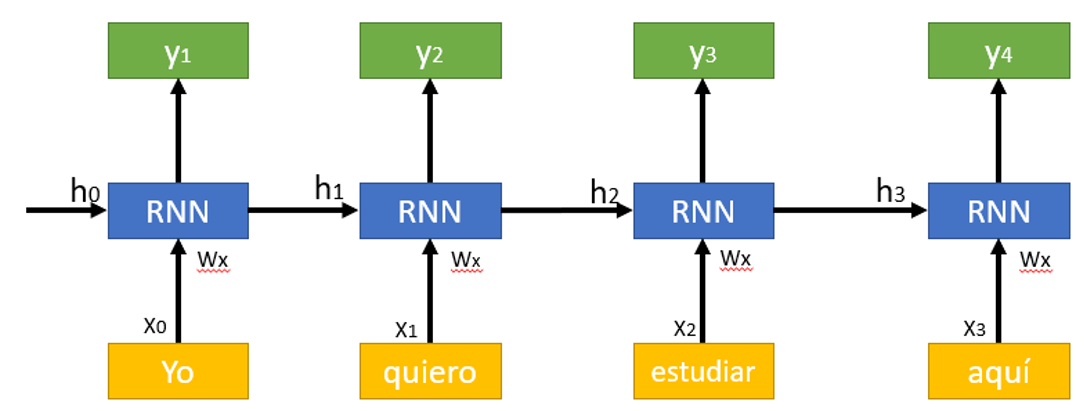
\includegraphics[width=0.8\textwidth]{figura2_8}
\caption{Representación de entrada y salida de una red recurrente }
\label{tab:figura2_8} 
\end{figure}

Las redes recurrentes son arquitecturas de aprendizaje profundo diseñadas para manejar datos secuenciales para poder retener los datos previos de la neurona. Esto permite al modelo preservar contexto y dar salida basados en datos previamente aprendidos. Una red recurrente toma ventaja de la naturaleza secuencial de la voz y el lenguaje, cada palabra es codificada con la información de la palabra previa. Un asistente virtual requiere mantener contexto para mantener una conversación y este factor de las redes recurrentes lo hace una elección altamente deseable para tareas NLP como generación de dialogo y reconocimiento de voz. Sin embargo, no todo son ventajas; existe un problema a cada paso creamos y entendemos de lo que leímos hasta ahora, así siempre es una mezcla de pasado y presente, a este problema se le denomina dependencia a largo término (Gaikwad, 2019).

\subsection{LONG SHORT TERM MEMORY}
El desafío de abordar la preservación de la información a largo plazo y la omisión de entradas a corto plazo en los modelos de variables latentes existe desde hace mucho tiempo. Uno de los primeros enfoques para abordar esto fue la memoria a largo plazo LSTM por sus siglas en inglés. Podría decirse que el diseño de LSTM está inspirado en las puertas lógicas de una computadora. LSTM introduce una celda de memoria (o celda para abreviar) que tiene la misma forma que el estado oculto (algunas literaturas consideran la celda de memoria como un tipo especial del estado oculto), diseñada para registrar información adicional. Para controlar la celda de memoria necesitamos varias puertas. Se necesita una puerta para leer las entradas de la celda. Nos referiremos a esto como la puerta de salida (Zhang et al., 2021).
\par
La figura 2.9 muestra como las memorias a largo y corto plazo tienen un estado adicional llamado estado de celda, por el cual la red hace ajustes en el flujo de información. La ventaja de este estado es que el modelo puede recordar u olvidar lo aprendido más selectivamente. Ya que LSTM permite a la red retener el estado de entrada por mucho, procesa largas secuencias muy eficientemente y rinde muy bien en términos de precisión (Gaikwad, 2019).


\begin{figure}[H]
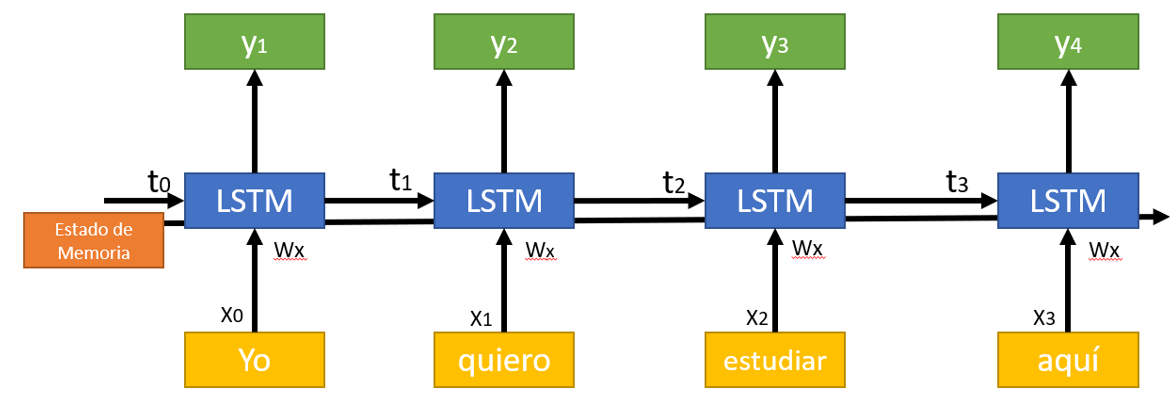
\includegraphics[width=0.8\textwidth]{figura2_9}
\caption{Representación de entrada y salida de una LSTM y su estado de memoria }
\label{tab:figura2_9} 
\end{figure}

Lane et al. (2019) afirma que: “El estado de la memoria se ve afectado por la entrada y también afecta la salida de la capa como en una red recurrente normal. Pero ese estado de memoria persiste en todos los pasos de tiempo de la serie de tiempo (su oración o documento). Entonces, cada entrada puede tener un efecto en el estado de la memoria, así como un efecto en la salida de la capa oculta. La magia del estado de la memoria es que aprende qué recordar al mismo tiempo que aprende a reproducir la salida, usando retro propagación estándar.”

\section{HERRAMIENTAS DE DESARROLLO}

Para realizar la implementación del prototipo del agente conversacional se recurrieron a diversas herramientas. A continuación en la tabla se mostrarán las distintas herramientas más importantes usadas en la fase de implementación.

\begin{table}[H]
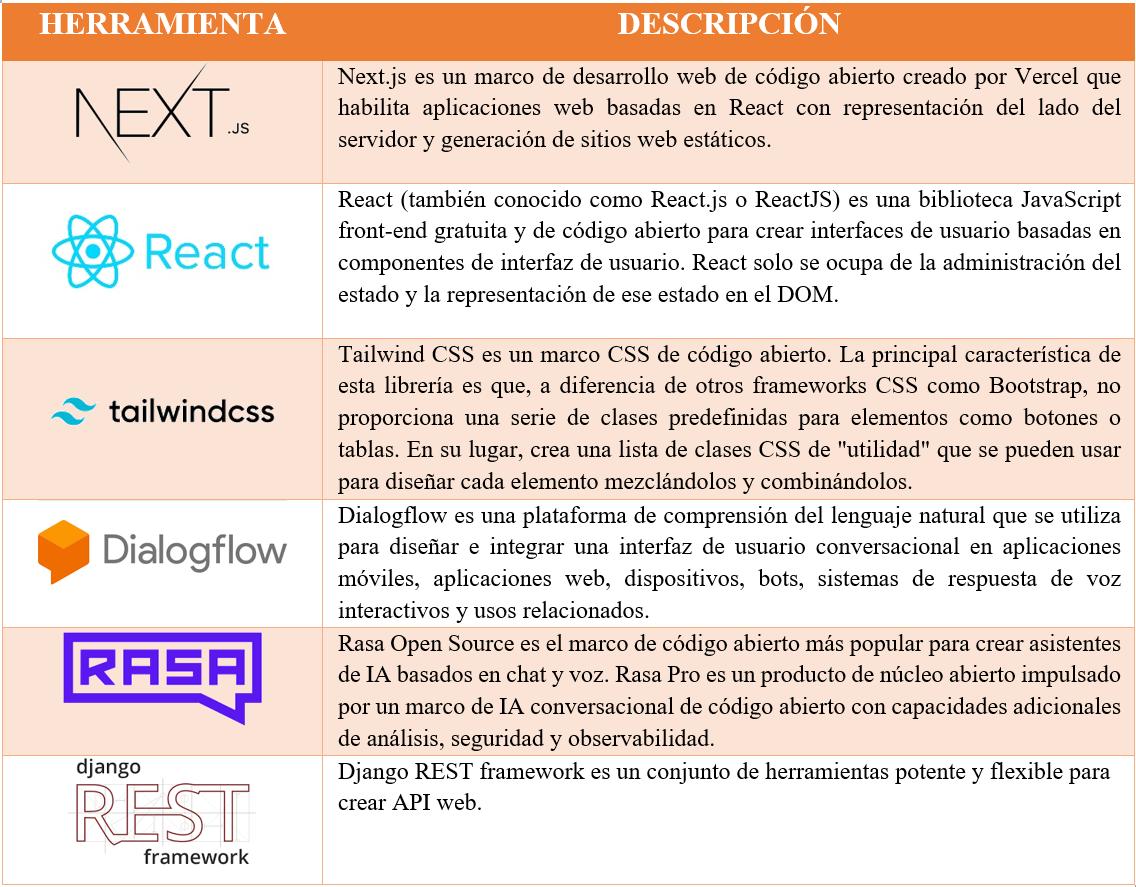
\includegraphics[width=1\textwidth]{tabla2_2}
\caption{Tabla de herramientas usadas en el desarrollo.}
\label{tab:tabla2_2} 
\end{table}

\section{COMPRENSIÓN DE TRÁMITES UNIVERSITARIOS Y ADMISIONES}

Según Gúzman A. (1999) un trámite se define como: "Un conjunto de operaciones relacionadas, ejecutadas por varias personas, que tiene un fin o propósito. Definidos como procesos distribuidos de manejo, almacenamiento y procesamiento de información dentro del ámbito de computación. Empero, la invención, supervisión y desarrollo de trámites han estado a cargo de personas no informáticas."
\par
La representación de un trámite se puede ver gráficamente como una red dirigida, cuyos nodos son actividades atómicas también llamadas tareas, cuyos arcos son entregables internos, con un nodo inicial y uno o más nodos finales (Palomino, 1999)
\par
La Figura 2.10 muestra un trámite enfocado a una solicitud de licencia de manejo, donde se pueden ver diferentes casos en cada nodo y las tareas que se debe seguir hasta llegar a algún nodo final. 

\begin{figure}[H]
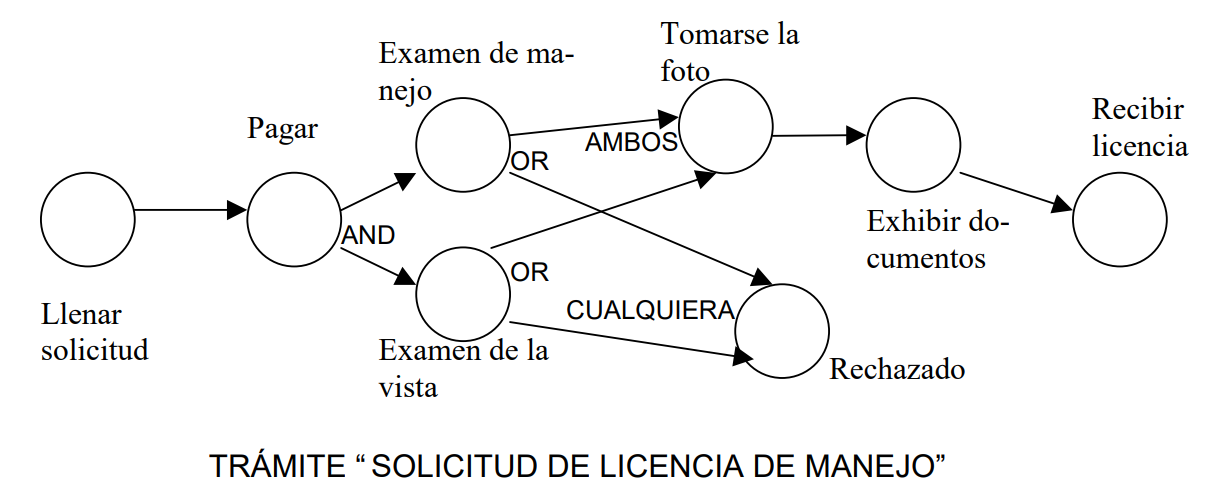
\includegraphics[width=0.8\textwidth]{figura2_10}\\
\setcaptioncitation{(Gúzman, 1999)}
\caption{Representación de un trámite}
\label{tab:figura2_10} 
\end{figure}

\subsection{RECOPILACIÓN DE TRÁMITES OBJETIVOS}
La Universidad Mayor de San Andrés tiene distintas unidades distribuidas tanto en rectorado y vicerrectorado; existen en estas unidades o divisiones ciertas actividades enfocadas a la atención de las necesidades académicas del público universitario. La siguiente lista describe el filtrado a las divisiones o unidades de interés inicial: 
\begin{itemize}
\item \textbf{División de títulos y diplomas}.- Cuya misión es procesar con eficiencia la atención de todos los trámites para la otorgación de títulos y diplomas a cargo de la Universidad Mayor de San Andrés.
\item \textbf{División de documentos y archivo}.- Tiene como objetivo 
organizar, conservar y difundir la documentación o información con valor administrativo, legal, fiscal o histórico, según disposiciones legales institucionales y nacionales. Difusión del patrimonio documental, a través del servicio de consulta e investigación del fondo documental y las series que la componen. 
\item \textbf{División de gestiones, admisiones y registros}.- Cuya función principal es viabilizar proceso de administración académica, referidos al régimen estudiantil, de acuerdo a normas vigentes, requisitos, programación y calendarios académicos e internos y otros previstos por instancias superiores.
\item \textbf{División de trabajo social}.- Cuyo objetivo es programar, organizar, gestionar y viabilizar la prestación de servicios sociales de calidad para estudiantes universitarios.
\item \textbf{División de salud}.- Cuya misión es contribuir a crear en la comunidad universitaria la cultura de la prevención y el autocuidado, mediante programas de promoción de la salud, medicina preventiva y servicios asistenciales, dando mayor énfasis a los sectores de bajos recursos.
\item \textbf{Admisiones de facultades y carreras}.- Para saber como se puede accedera una carrera se deben tener en cuenta las distintas modalidades y puntos de atención.
\end{itemize}

Acotando la búsqueda de información a los anteriores puntos se procede a revisar cada división o unidad en búsqueda de trámites relacionados al pre grado, filtrando y destacando los nodos a tomar en cuenta para cada trámite. 

\subsection{DIVISIÓN DE TÍTULOS Y DIPLOMAS}

Para la búsqueda de información se accedieron a las páginas de redes sociales, como a la página oficial de la división de títulos y diplomas; de las cuales se obtuvo en orden los siguientes trámites que podran ser de interés.

\begin{enumerate}[label=(\alph*)]
\item \textbf{Apostilla certificación única de documentos}.- El Ministerio de Relaciones Exteriores, desde la implementación de la Apostilla Digital, tiene a disposición de los ciudadanos el sitio web que cuenta con información detallada referente a dicho servicio, como también con tutoriales de fácil acceso. 
\begin{itemize}
\item Información principal.- Se considera usar la siguiente información sobre el inicio del trámite: “La Apostilla es un certificado que permite reconocer los documentos públicos bolivianos en el exterior y suprime la exigencia de legalización de documentos públicos extranjeros en el país y será verificada desde cualquier parte del mundo”. Además el enlace a la página oficial del trámite de apostilla.
\item Solicitud de apostillado.- El ministerio ofrece un video con la información necesaria para iniciar con los documentos necesarios, se ofrece enlace del video, además de la página donde se podrá iniciar la solicitud de apostilla. 
\item Seguimiento de la apostilla.- También se muestra un video de como poder seguir el trámite de forma remota y la página donde se debe realizar este mismo.
\item Pago y verificación de apostilla.-Para ambos casos se muestran los videos correspondientes a dicho trámite, además de sus enlaces correspondientes.
\item Puntos de atención.- Se consideran los puntos físicos de atención como son: la división de títulos y diplomas incluyendo su horarios de atención. 
\item Páginas de información.- Tanto la página oficial como la de Facebook se difundirán en el chatbot como también los números de atención,  para el ministerio se ofrece la página con puntos de atención.
\end{itemize}

\item \textbf{Extensión de diploma académico y titulo profesional simultaneo}.- Con modalidades de graduación: Excelencia, Tesis de Grado, Trabajo Dirigido, Internado Rotatorio, Examen de Grado, Proyecto de Grado, Tesina, Monografía, Pasantía, Proyecto de Grado Técnico.
\begin{itemize}
\item Inicio trámite.- Se ofrece un video de solicitud de trámite simultaneo: en la página de trámites en línea donde se puede iniciar un trámite
\item Costos.- Se puede mostrar la siguiente vista de costos: Diploma académico – título profesional (simultaneo) técnico universitario superior Bs. 1.567.- • Diploma académico – título profesional (simultaneo) nacionales licenciatura Bs. 2.820.- • Diploma académico – título profesional (simultaneo) extranjero licenciatura Bs. 5.765.- • Modalidad graduación por excelencia académica solo cancela legalización de resolución Bs. 129
\item Requisitos de diploma académico o título profesional.- Para revisar los requisitos del diploma académico se ofrece un documento donde se explica a detalle cada requisito.
\item Más información.- El cronograma de recepción de documentos y entrega de diplomas académicos y profesionales, será difundido en redes sociales. Se ofrece alternativamente la ubicación en \textit{google maps}.
\end{itemize}

\item \textbf{Diploma Académico}.- Para definir la estructura de este trámite se recomienda que el primer nodo sea informativo sobre que es y cuando se requiere; tratar se considera resumir: El Diploma Académico es un documento que se requiere para realizar el trámite del Título en Provisión Nacional Universitario de cualquier Carrera Universitaria y en cualquier universidad pública de Bolivia, esta dirigido a los universitarios que hayan concluido sus estudios universitarios en pre-grado y rendido satisfactoriamente el examen de tesis o cumplido con cualquiera de las modalidades de egreso.
\begin{itemize}
\item Requisitos previos.- Para la presentación de documentos, ingresar a la página de trámites en línea, y ver los requisitos que se deben cumplir. 
\item Costos.- Entre los costos más importantes a considerar: esta el formulario de solicitud de trámite diploma académico: Nacional a 1008 Bs, Extranjeros 1998 Bs, Técnico Superior 515 Bs, también Certificado de calificaciones de grado: puedes revisar el detalle en el enlace “Ver requisitos” o coordinar los costos en el enlace “Tabla de valores”.
\item Más información.- Copnsiderar preguntar en el edificio Melissa para más detalles, adjuntar \textit{google maps}.
\item Fechas.- Una vez cumplido la conclusión de estudios y cumplido con la modalidad de egreso puedes iniciar tu trámite; generalmente la información se ofrece de Kardex de cada carrera; también puedes revisar el enlace “Página Facebook” donde actualizan cualquier detalle.
\end{itemize}

\item \textbf{Título profesional}.- El Título Profesional, es el único documento que acredita el ejercicio legal de la profesión en el Estado Plurinacional de Bolivia. Considerar la página “Ver detalles”.
\begin{itemize}
\item Costos.- El costo del trámite para Nacionales licenciatura: 1683 Bs., Extranjeros: 3638 Bs. Y técnico medio y superior 923 Bs.; el costo incluye formulario de solicitud de trámite.
\item Requisitos.- Sobre los requisitos se debe tener en cuenta que es exclusivo para título profesional y la cita previa en el enlace “Cita previa” también haber leído toda la información necesaria.
\item Cronograma.- El último punto 13 en la sección de requisitos del enlace  “Ver requisitos” contiene la fecha actualizada para presentación de documentación.
\item Más información.- La atención y recepción se efectúa de manera mensual en horarios según último comunicado en la página “Títulos Umsa” 
\end{itemize}

\item \textbf{Certificado supletorio}.- El certificado de supletorio es otorgado en casos de extravío certificado otorgado en caja recaudadora “Edificio Melissa”, deterioro o roba del Diploma Bachiller, Académico y Título Profesional, estos dos últimos SOLO si fueron otorgados por la UMSA.
\begin{itemize}
\item Requisitos.- Tener en cuenta los gastos correspondientes del formulario de solicitud de trámite, fotocopia del título; en caso de pérdida presentar certificación emitida por FELCC sobre perdida o robo; para más detalles revisar y leer “Ver Requisitos”.
\item Atención.- Para más información o inicio del trámite mensualmente se realiza la atención; de acuerdo a comunicado publicado en la página “Ver Trámites Títulos”
\end{itemize}
\end{enumerate}

\subsection{DIVISIÓN DE DOCUMENTOS Y ARCHIVO}

Se consideraron los siguientes servicios a universitarios de pre grado. 
\begin{enumerate}[label=(\alph*)]
\item \textbf{Firma digital apostillado}.- La firma digital es un requisito para la apostilla de documentos, validando el documento fuera de territorio nacional.
\begin{itemize}
\item Costo.- El costo de la firma digital en Fotocopia legalizada es de 26Bs y en documento Original 203 Bs.
\item Donde.- Solicite la firma digital para el apostillado en ventanilla “Legalizaciones” segundo patio Monoblock Central horario de atención 8:30 en adelante.
\item Requisitos.- Después de presentación de documentos original y fotocopia anverso y reverso tamaño oficio recabar el sello de autorización para pago de valores “Ver tabla de valores”, recabar la boleta y entregar en ventanilla el sello de pago: Para más detalles ver “Requisitos firma”.
\end{itemize} 

\item \textbf{Legalización}.- Para legalizar cualquier documento considerar dos formas una “en línea” haz click “requisitos en línea” o “presencial”.
\begin{itemize}
\item En línea.- Acceder a la página “Cita previa legalización” o acceder al archivo “Guía de legalizaciones”, también si ya revisaste los dos anteriores revisar también “Solicitud de formulario trámite”.
\item Presencial.- En ventanilla de legalizaciones debe presentar cedúla de identidad y  Título o Diploma original y fotocopias anverso y reverso tamaño oficio, una vez presentados recabar el sello de autorización para el pago de valores “Ver tabla de valores” según su legalización correspondiente; luego puede seguir más detalles en “Ver requisitos ”.
\item Costos.- A continuación la imagen muestra los costos de cada fotocopia, considere su tipo de trámite considere imagen tabla de valores.
\item Perdida boleta.- La reposición de lo cancelado 17Bs en el tesorio Universitario.
\item Quienes.- Solo podrá realizar el trámite el interesado o parientes en primer grado; o conyugues con certificado de matrimonio o libreta familiar y/o terceras personas con poder notariado
\end{itemize}
\end{enumerate}

\subsection{DIVISIÓN DE GESTIONES, ADMISIONES Y REGISTROS}


Para esta división se tomaron en cuenta la siguiente lista de trámites:

\begin{enumerate}[label=(\alph*)]

\item \textbf{Matriculación}.- Es un registro de los datos personales de un individuo de manera específica, en un archivo con la finalidad de ingresar al sistema universitario. 
\begin{itemize}
\item Requisitos.- Todo individuo habiendo aprobado alguna modalidad para el ingreso a una carrera en la universidad podrá iniciar su trámite de matriculación: Si se matricula por primera vez en el sistema universitario siga el enlace "Alumno nuevo" sino siga el enlace "Alumno Antiguo"
\item Costo.- El pago de valor de matrícula tiene un costo para alumnos Nacional o Normalista de 27 Bs., Profesionales de 245 Bs., Extranjero de 1680 Bs y rezagados de 182 Bs,. Recordar que cada facultad acordará el aporte facultativo, consulta en los predios de tu facultad. Ver pago CPT.
\item Nuevo.- Para los alumnos nuevos deberás considerar la serie de pasos para la matriculación puedes ver el enlace "Ver requisitos", también puedes ver el video tutorial "Tutorial matriculación universitaria"
\item CPT.- El pago CPT es una forma de pagar en línea desde un UniNET o banca móvil, puedes revisar el siguiente video "Código de pago de trámites"
\item Cronograma Nuevo.- En la página de división de gestiones se encuentra el cronograma actualizado de matriculación "Ver cronograma".
\item Antiguo.- Puedes proceder a pagar el valor de la matrícula y tu aporte facultativo si es que se tuviera; este pago es único por año, revisa el enlace "Costo matricula"

\item Mas información.- La página "Ver Gestiones" contiene la información reciente sobre las matriculaciones, también puede ir a la dirección referida a continuación para informarse personalmente, vea la imagen de referencia "Matriculación ventanilla 8"

\item En línea.- Para la certificación en línea de la matricula universitaria considere en enlace "Ver requisitos" donde se muestra la serie de pasos a seguir 
\end{itemize}

\item \textbf{Modalidades de graduación}.- A continuación se generalizan los distintas modalidades de graduación, por cada caso se direcciona a un pdf con los requisitos al parecer estático, ver cambios. 
\begin{itemize}
\item Grado técnico superior.- Para estudiantes que habrían realizado el examen de grado referirse al enlace "Ver TUC examen" y para aquellos que realizaron una pasantía referir "Ver TUC pasantía"
\item Graduación directa.- Para la modalidad de graduación directa siga los requisitos y el procedimiento en el enlace "Ver graduación directa"
\item Contador general.- Para contador general puede revisar los requisitos y procedimientos "Ver contador general"
\item Técnico medio.- Si la modalidad es de técnico medio puede revisar los requisitos y el procedimiento en el enlace "Ver técnico medio"
\item Bachelor.- Para bachiller superior revise los requisitos y el procedimiento a seguir en el enlace "Ver bachelor"
\item Tesis, tesina y proyecto de grado.- Según la modalidad de tesis, tesina o proyecto de grado el inicio del trámite como requisitos se encuentran en el enlace "Tesis, tesina y proy. grado"
\item Continua las siguientes modalidades. 
\item Costo.- Para cada caso referir la tabla de valores para los distintos formularios necesarios como GAR 101, fotocopias legalizadas, etc. "Ver tabla valores"
\item Consulta.- Por su carnet de identidad se puede consultar el trámite correspondiente a GAR, seguir el siguiente enlace "Consultar trámite".
\end{itemize}

\item \textbf{Carrera paralela}.- Una carrera paralela implica gestionar dos carreras a la vez cumpliendo los requisitos de materias aprobadas y promedio de 65\%, o completado el 80\% de su plan de estudios; pueden iniciar su trámite de carrera paralela. 
\begin{itemize}
\item Requisitos.- Los requisitos para la carrera paralela  pueden ser revisados en el enlace "Ver carrera paralela".
\item Procedimiento.- Se publicarán y actualizarán para el ingreso al  siguiente semestre en currso en la tabla "Plazas y Calendario", si hubiere pasado el plazo se deberá esperar al siguiente semestre. La actualización sucederá en el transcurso de cada semestre puedes estar atento a la página "Ver paralela" en el transcurso de tu semestre. 
\item Cronograma.- Si revisaste "Plazas y calendario", recuerda que el día mencionado a esas horas debes apersonarte con la documentación necesaria en la ventanilla "Introduce ventanilla".
\item Información y trámite.- Para proceder con la entrega de documentación o consultar sobre los requisitos, dirigete a la ventanilla mostrada en la imagen. 
\item Rezagados.- En caso de ser rezagado debe dirigirse a la ventanilla, donde le indicarán que día entregarán los resultados de las plazas y si existiese una plaza para usted. Caso contrario deberá esperar al semestre o año según corresponda.  
\end{itemize}

\item \textbf{Traspasos}.- Los traspasos corresponden al mismo sistema universitario nacional o local dentro de la universidad, también externo modalidad pasantía.
\begin{itemize}
\item Cambio de carrera.- Si desea realizar el cambio de carrera a uno correspondiente de la universidad, considere revisar los requisitos y procedimientos. "Ver cambio"
\item Traspaso a universidades del sistema.- Considere como universidades del sistema a toda universidad de convenio universitario público: UAGRM, UMSS, UPEA, revisar sistema. 
\item Información.- Para más información acerca de cambios de carrera o traspasos en general "Ventanilla 13"
\end{itemize}

\subsection{TRABAJO SOCIAL}
Para la división de trabajo social se consideran los siguientes trámites con más relevancia en el conjunto universitario de pre grado.
\begin{enumerate}[label=(\alph*)]

\item \textbf{Beca Comedor}.- Consiste de apoyo alimentario que la Universidad Mayor de San Andrés brinda a los estudiantes universitarios destacados y con situación social económica precaria.
\begin{itemize}
\item Requisitos.- Cómo requisitos previos fundamentales se toma en cuenta que el estudiante debe vencer todas las materias correspondientes al primer semestre o año en su carrera de origen no paralelas, no estar en internado rotatorio o beca académica de más de 40 Hrs/mes y no aportar a AFP's para más detalle vea "Ver requisitos"
\item Procedimiento.- Para los requisitos y documentos a presentar revise el enlace "Ver requisitos"
\item Información.- Puede revisar la página informativa "Ver beca comedor" y las redes sociales "Trabajo Social"; también puede acudir de manera presencial revisar "Imagen trabajo social".
\end{itemize}
\end{enumerate}

\end{enumerate}


\chapter{MARCO APLICATIVO} 

Este capítulo especifica el desarrollo del proyecto de agente inteligente para preguntas frecuentes de los trámites universitarios de pre grado y hará uso de la metodología de desarrollo ágil aplicando el {\it framework scrum}, especificando primero el {\it product backlog}, estableciendo metas y realizando el refinamiento en tareas más pequeñas que representen iteraciones significativas dando un producto funcional y disponible para lanzamiento desde la primera iteración, implementando primero una interfaz de interacción con el usuario final. \par
Se adapta la metodología y el desarrollo a una persona, ejerciendo los roles que componen al desarrollo empezando por el cumplimiento de los eventos, artefactos y reglas que realizaría el {\it scrum master} y siguiendo una estructura de tareas definidas para un product backlog y saber que se debe hacer en cada iteración, estableciendo tiempos de entrega y comunicación continua con los usuarios a través de entrevistas y mejora en cada reunión diaria por la necesidad de interacción que requiere la creación de un sistema de agente conversacional. 

\section{FASE PRE-GAME}
\subsection{DEFINICIÓN DE { \bf  PRODUCT BACKLOG}}

Esta fase deberá considerarse ser la base de interacción principal se deben considerar todos los elementos que compondrá el desarrollo del producto, teniendo en cuenta las funcionalidades y requisitos en forma de lista priorizada. Para lograr este objetivo se suele hacer uso de historias de usuario que describa claramente los requisitos funcionales para el usuario, siguiendo la estructura de la Figura 3.1 se muestra el formato de la historia de usuario que describen las funcionalidades resultado de la interacción de universitarios en el predio de la Universidad, páginas de difusión social y propias de cada división, como también comentarios de administrativos a cargo de dar la información personal de los trámites de pre grado realizados día a día por la comunidad estudiantil. 
\begin{figure}[htb]
\centering
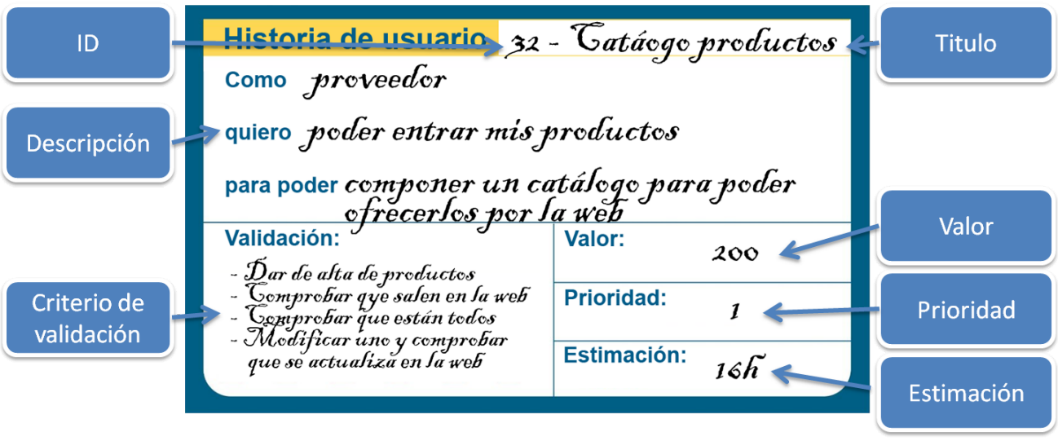
\includegraphics[width=1\textwidth]{figura3_1}
 \setcaptioncitation{(Menzinsky, 2016)}
 \caption{Ejemplo componentes de una historia de usuario}
\label{fig:figura3_1}
\end{figure}
\par
La lista de requerimientos pueden ser tareas técnicas o más centradas al usuario, se ordenará la siguiente lista a nivel de prioridad, esta lista principal de requerimientos puede ser modificada y re ordenada en prioridad al final de un {\it sprint}. 
\subsection{DETECCIÓN DE PÚBLICO OBJETIVO}
\par
En el marco de investigación aplicativa el desarrollo no cuenta con experiencia previa en ninguna de las ramas afines a la Universidad Mayor de San Andrés que hacen gestión y administración de toda la comunidad estudiantil de pre grado, debido a lo posterior es necesario definir el público objetivo y viabilidad de obtención de información por los medios públicos que se posean, y no así de carácter administrativo. Dado esto se establece que el usuario final objetivo son todos los estudiantes que realizan consultas en los predios de atención de los distintos puntos descritos en la recolección de información. 
\subsection{ESTRATEGIA DE RECOPILACIÓN DE REQUERIMIENTOS}
Para poder reunir los requerimientos de las preguntas más frecuentes que realiza un universitario, es necesario recurrir a la técnica de la entrevista; conociendo los documentos que cada división gestiona y es de interés para el usuario. Dado un análisis previo de las consultas más comunes realizados en un sondeo de preguntas, se trabajo con las siguientes preguntas: \par
\begin{itemize}
\item ¿Qué trámite o documento estás realizando?
\item ¿Cómo obtuviste información sobre los requisitos, costos o las características que tiene el trámite que realizas?
\item ¿Conocías la página de información respecto a tu trámite?
\item ¿Te sería útil un asistente virtual que pueda responder a algunas de tus dudas?
\end{itemize}
Debido a la variabilidad de trámites realizados día a día en los distintos puntos de atención de cada una de las divisiones que son concernientes a la investigación. Siendo un marco de inicio para obtener los requerimientos funcionales, también se encontraron páginas referentes a la información pública que se tiene sobre cada tramite, la segunda estrategia a seguir fue la observación de los distintos puntos de consulta que existen y se llegó a la conclusión que los trámites o información más requerida respecto a estos son: 
\begin{itemize}
\item División de títulos y diplomas
\item División de documentos y archivo
\item División de gestiones, admisiones y registros
\item División de trabajo social
\item División de salud y servicios psicológicos
\item Sección de Becas 
\end{itemize}

\begin{figure}[htb]
\centering

\includegraphics[width=0.7\textwidth]{figura3_2}
 \setcaptioncitation{(Portal GAR, 2022)}
 \caption{Portal web de la división de gestiones admisiones y registros}
\label{fig:figura3_2}
\end{figure}

\par
En gran medida los trámites más comunes realizados por universitarios de pregrado se basan en las consultas de requisitos, costos, direcciones, información adicional y horarios de atención, se encontró que gran parte de los encuestados desconocía de las páginas de atención que cada división presenta ya sea en redes sociales o páginas web, como se muestra en la Figura 3.2, la división de gestiones, admisiones y registros tiene su página donde se puede encontrar los distintos tramites que gestionan junto con sus requisitos y comunicados. 



\par
\section{HISTORIAS DE USUARIO}
Para conocer cuáles son los requisitos que debe cumplir la aplicación se  generarán historias de usuario que definan lo que se quiere lograr para poder refinar las tareas a posterior. 

\hfill

\begin{table}[!ht]
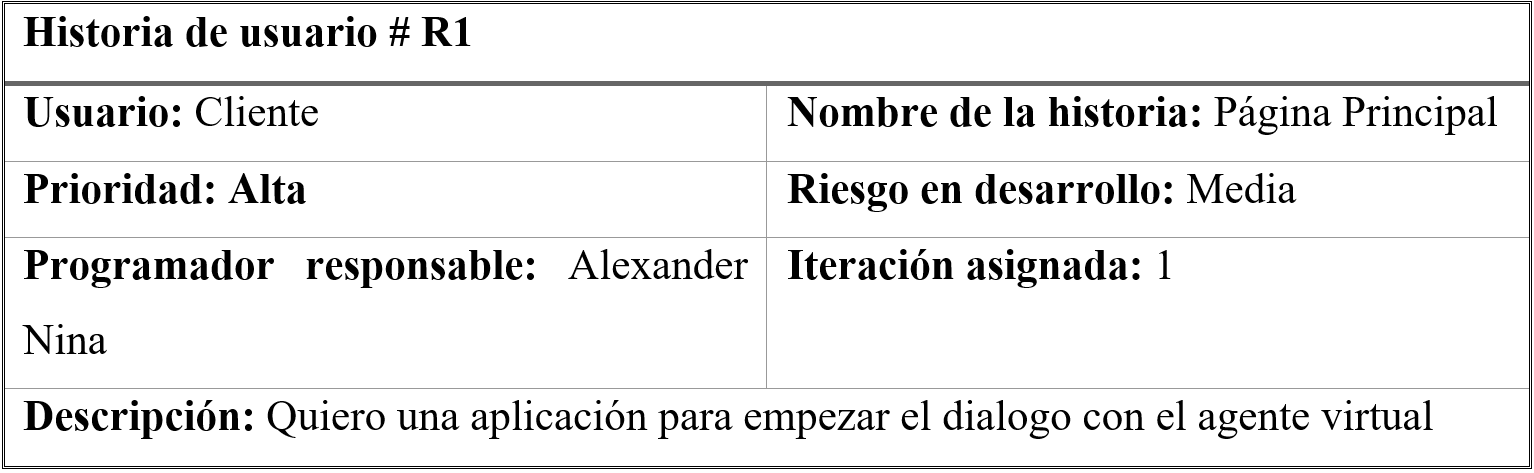
\includegraphics[width=1\textwidth]{tabla3_1}
\caption{Historia de usuario página principal} 
\label{tab:tabla3_1} 
\end{table}

\par
Como se muestra en la tabla 3.1, se busca mostrar una interfaz principal con la información más importante que puede trabajar un usuario, lo que puede hacer con el asistente, como acceder a una conversación y lo que es más importante para el desarrollador si el usuario quiere ofrecer una sugerencia o considerar un fallo en la aplicación {\it web}.

\begin{table}[!ht]
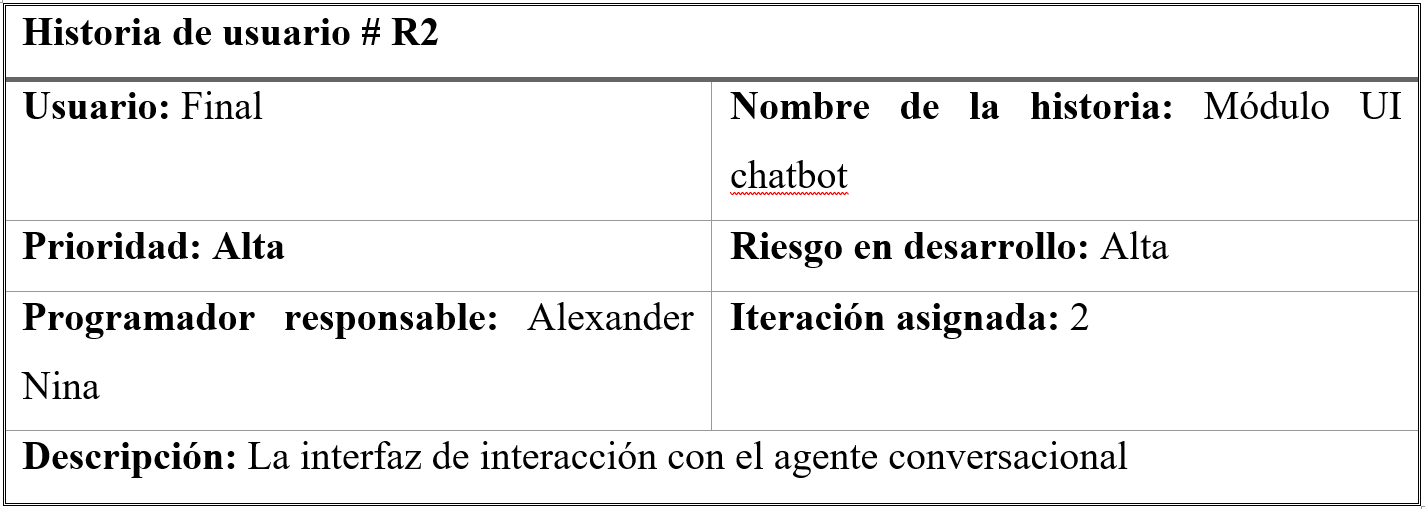
\includegraphics[width=1\textwidth]{tabla3_2}
\caption{Historia de usuario interfaz agente conversacional} 
\label{tab:tabla3_2} 
\end{table}

\par
Para la tabla 3.2, se debe desarrollar un componente de interfaz amigable para el usuario, que sea cómodo y siga un estándar en las aplicaciones de mensajería más populares, para esto se sigue un diseño y maquetado bien definido. 


\par
La tabla 3.3 indica la necesidad de conectar el módulo de mensajería con la plataforma como servicio seleccionado por administrador, pero considerando la primera iteración se usará y construirá en base a la plataforma {\it dialogflow} en fases de prueba del proyecto evita la carga en servidor público para su uso, en lugar de montar un servicio sin datos de uso como flujos conversacionales confirmados o un diccionario de palabras. 

\begin{table}[!ht]
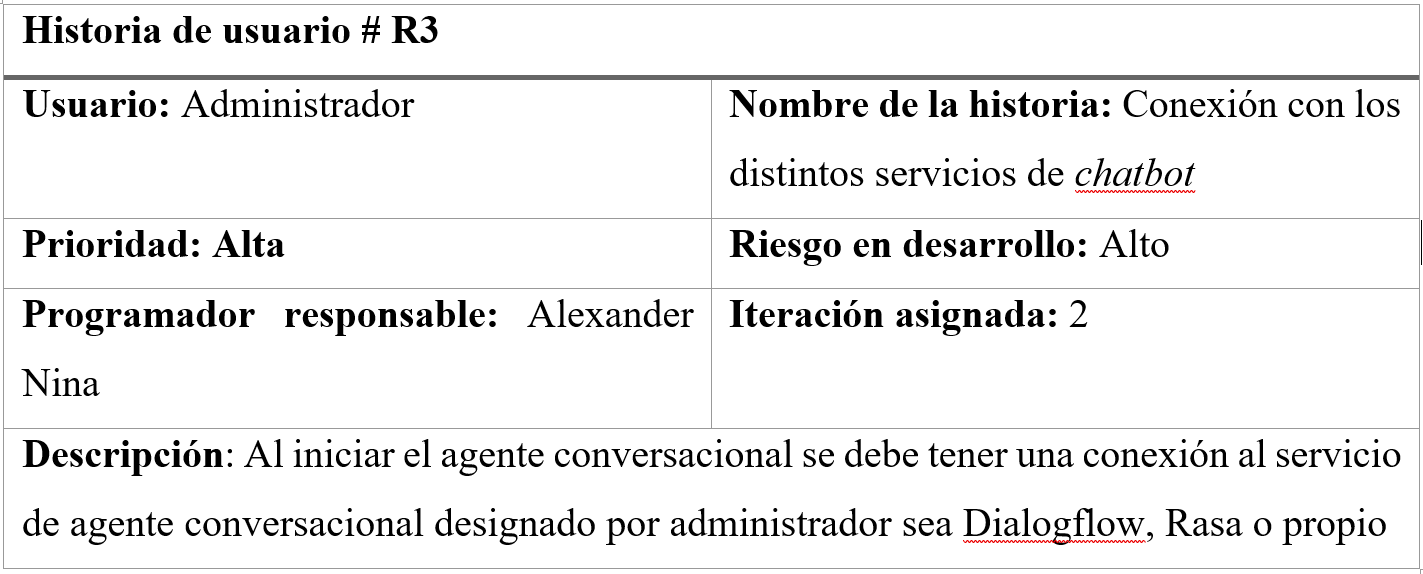
\includegraphics[width=1\textwidth]{tabla3_3}
\caption{Historia de usuario conexión con servicios y base de datos} 
\label{tab:tabla3_3} 
\end{table}

\par
A medida que se realizaba la investigación de las distintas alternativas para construir {\it chatbots} se encontró en las dos opciones que se consideran en este documento que tanto {\it dialogflow} como {\it rasa} tienen una alternativa de paga para diseñar circuitos conversacionales de manera gráfica, al desarrollar algún circuito conversacional en las versiones gratuitas de estos se noto la dificultad de esta construcción, además de la necesidad de almacenar la información en una base de datos, se desarrolla una construcción de un {\it builder} gráfico haciendo uso de la API de {\it dialogflow} para {\it NodeJS}.

\begin{table}[!ht]
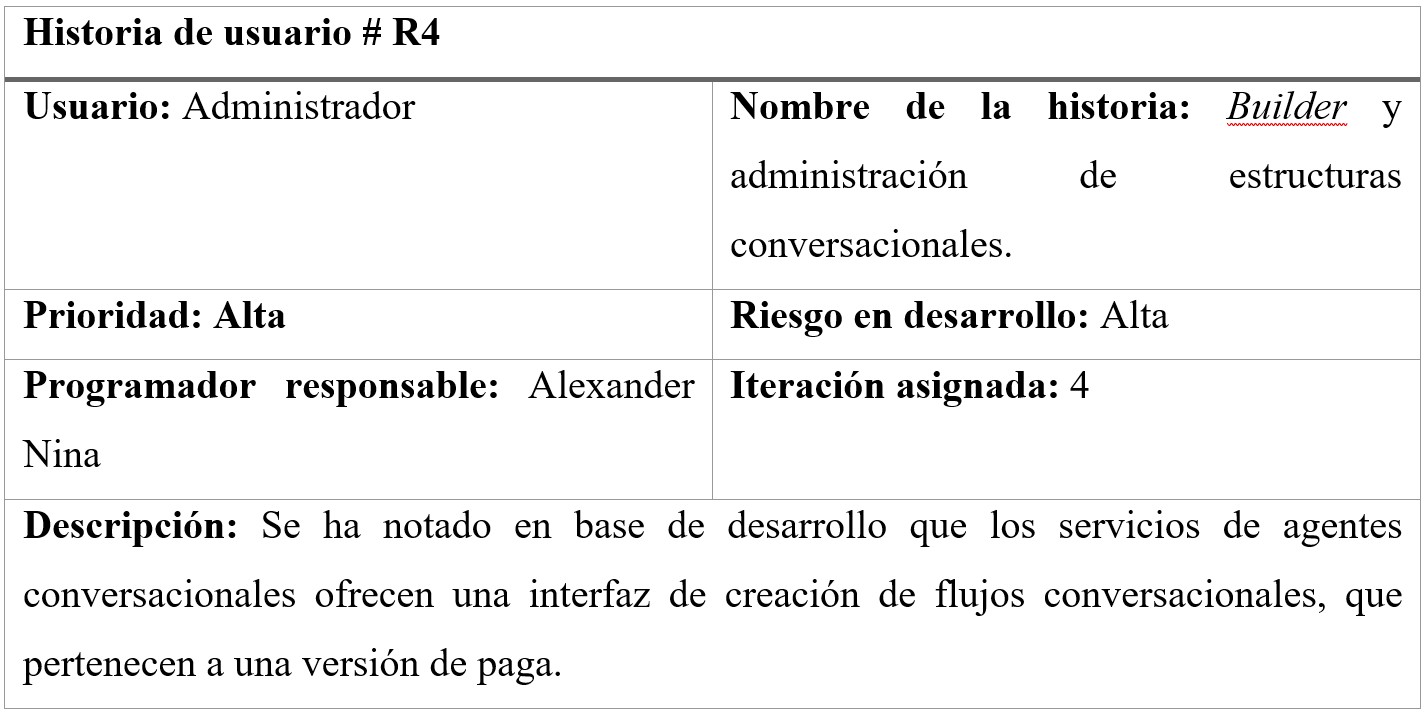
\includegraphics[width=1\textwidth]{tabla3_4}
\caption{Historia de usuario generador gráfico de circutos conversacionales. } 
\label{tab:tabla3_4} 
\end{table}

\par En la tabla 3.5 se pretende construir el primer flujo conversacional, aplicando las buenas prácticas que ofrece la metodología IMADTC explicada en el capitulo anterior. Siguiendo la construcción de las conversaciones en la tabla 3.6 se consideran las legalizaciones como un trámite cotidiano realizado por la comunidad universitaria.
Cada historia de usuario posterior correspondiente a la construcción de conversaciones seguirá la misma estrategia que se conducirá por la búsqueda de información que el asistente no pudo reconocer. 

\begin{table}[!ht]
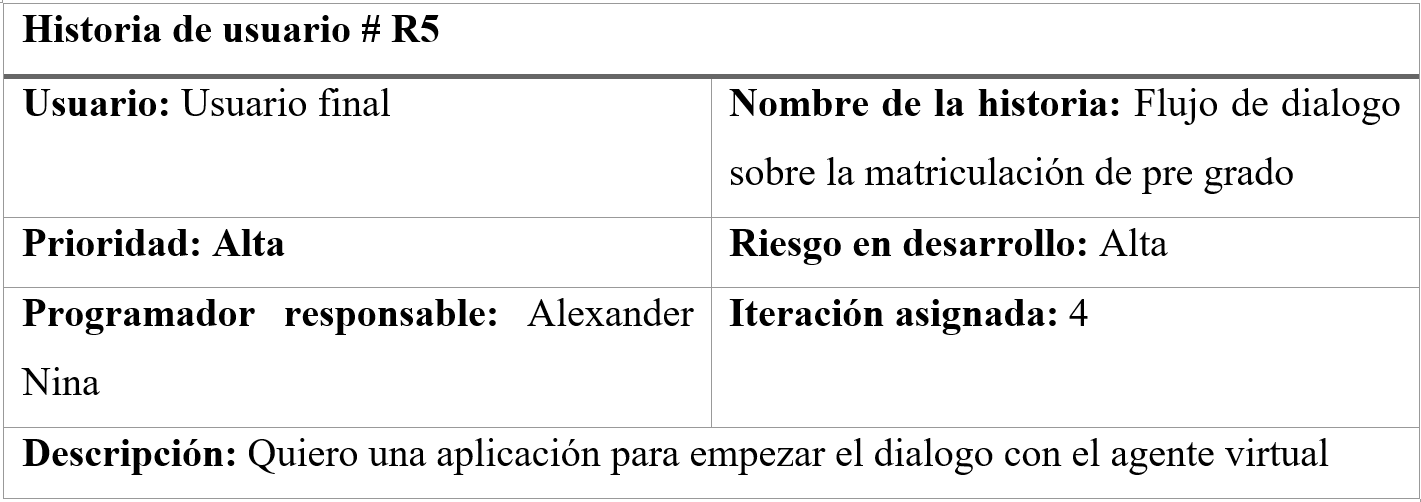
\includegraphics[width=1\textwidth]{tabla3_5}
\caption{Historia de usuario flujo de dialogo sobre la matriculación. } 
\label{tab:tabla3_5} 
\end{table}

\begin{table}[!ht]
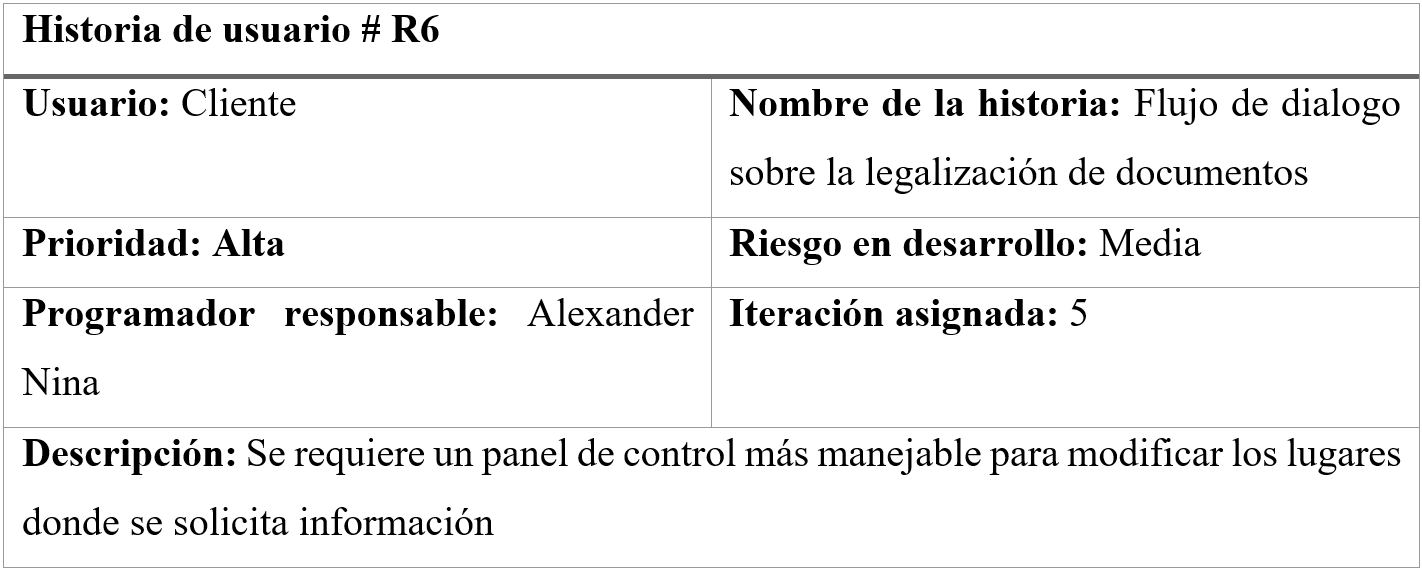
\includegraphics[width=1\textwidth]{tabla3_6}
\caption{Historia de usuario flujo de dialogo sobre la legalización de documentos. } 
\label{tab:tabla3_6} 
\end{table}

\section{PILA DEL PRODUCTO}

Cada historia de usuario debe seguir el criterio INVEST, siendo independiente, negociable, estimable, de tamaño específico y comprobable en cada {\it sprint}, en el marco de desarrollo ágil SCRUM engloban los requerimientos funcionales que debe tener el agente conversacional para poder garantizar la definición de hecho por sus siglas en inglés {\it definition of done} de cada {\it sprint} se propone el siguiente {\it product backlog}.

\begin{table}[!ht]
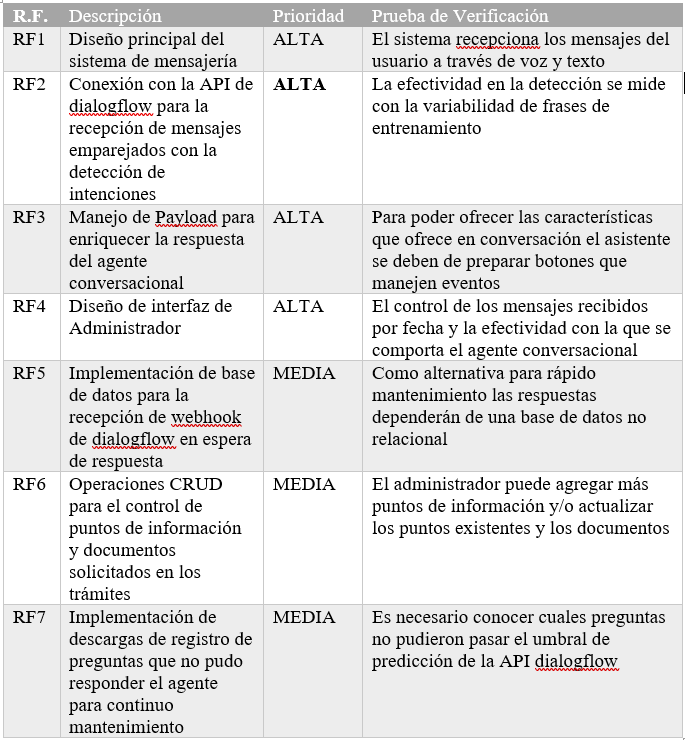
\includegraphics[width=1\textwidth]{tabla3_7}
\caption{Construcción del {\it product backlog}. } 
\label{tab:tabla3_7} 
\end{table}

\section{FASE GAME}

En la fase de desarrollo se explicará como se trabajó cada sprint teniendo en cuenta la característica iterativa del producto en base a la mejora continua, midiendo la cantidad de tiempo asignada para cada tarea. Al tratarse de una aplicación {\it web} se adopta el modelo de metodología UWE en cada iteración haciendo uso de sus herramientas: casos de uso, modelo de base de datos, diagramas de secuencia, diseño, presentación y navegación. 
\par
Además de las técnicas presentadas en el marco teórico teniendo en cuenta que se trata de un agente conversacional se tomarán algunas técnicas de la metodología {\it IMADTC} ya habiendo usado en la fase de pre game la contextualización del agente conversacional en su dominio, en esta sección es interesante para los {\it sprints} un diseño del flujo conversacional, ya que la ventaja de usar un servicio API como dialogflow es poder hacer uso del contexto para que el asistente sea capaz de entender preguntas abiertas como se muestra en la figura 3.3. 

\begin{figure}[htb]
\centering
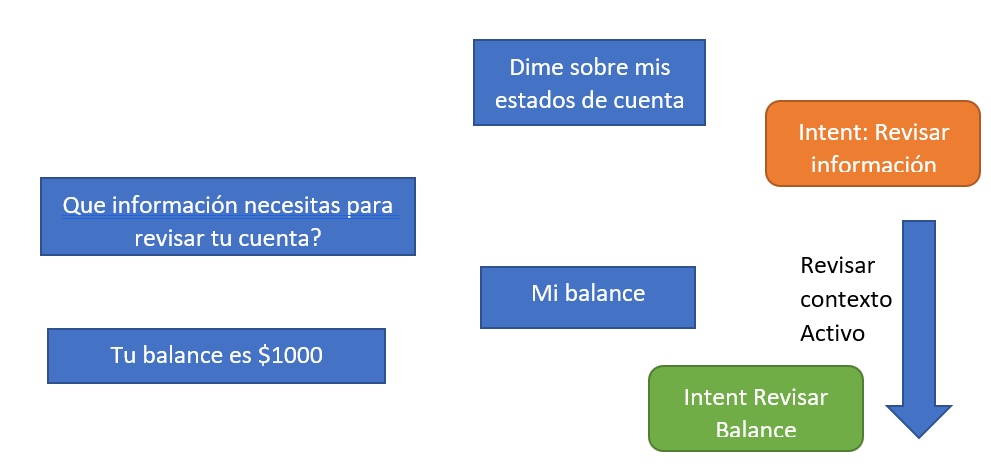
\includegraphics[width=0.9\textwidth]{figura3_3}
 \setcaptioncitation{(Documentación dialogflow, 2022)}
 \caption{Ejemplo de flujo contextual de dialogflow.}
\label{fig:figura3_3}
\end{figure}

\par
La técnica que corresponde al diseño del flujo conversacional es la cuarta fase en la metodología {\it IMADTC}, sugiere que con la información recabada hasta el momento del desarrollo, se requiere de un esquema representativo de la conexión de las tareas encontradas como parte de los escenarios encontrados en las historias de usuario, el objetivo del esquema es ser un esqueleto para la lógica que deberá seguir el agente conversacional para clasificar mejor su respuesta, y al mismo tiempo que se tiene una representación visual del flujo de la conversación con el usuario en un diagrama de flujo. Siguiendo la notación de la ISO 5807 para la documentación de los símbolos y convenciones para los datos, programas y sistemas de flujo, establece el significado de los símbolos en la figura 3.4. 

\begin{figure}[!ht]
\centering
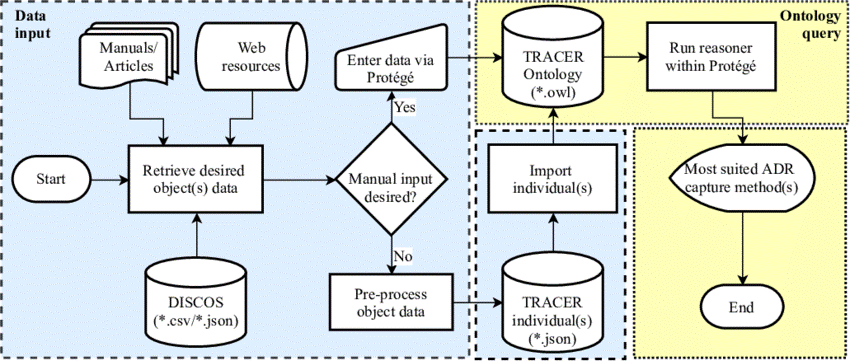
\includegraphics[width=0.9\textwidth]{figura3_4}
 \setcaptioncitation{(Yüksei, 2020)}
 \caption{Ejemplo de las estructuras definidas en la ISO 5807.}
\label{fig:figura3_4}
\end{figure}

\section{PRIMERA ITERACIÓN}

Para poder realizar la primera iteración se tendrá en cuenta las historias de usuario más importantes o de alto requerimiento, también se debe definir los modelos de la interfaz de usuario pública con la que se podrá conversar a través de voz y texto, siguiendo la metodología {\it UWE} con los distintos modelos con los que se mostrará a continuación, siendo esta primera iteración la interfaz y experiencia del usuario final y poder mejorar sobre la marcha en la figura 3.4 se definirá el sprint backlog, definida en la tabla 3.8.

\begin{table}[ht]
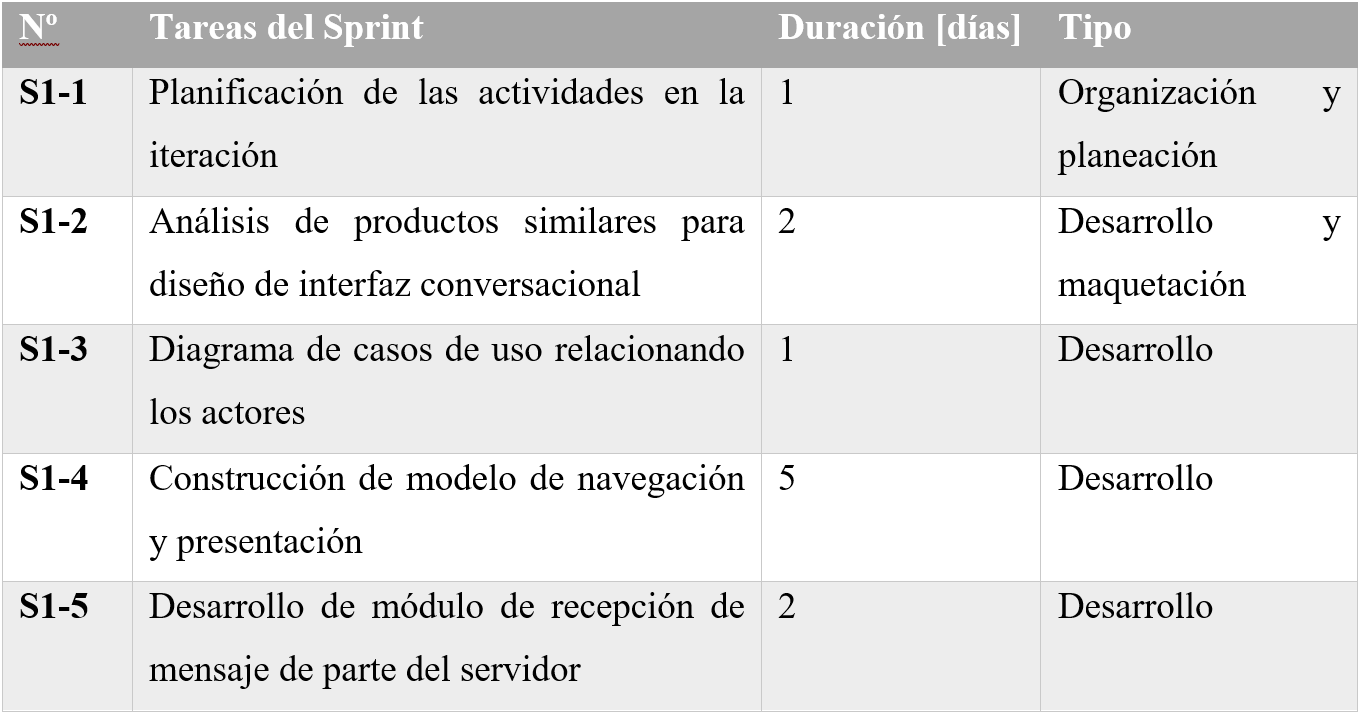
\includegraphics[width=1.1\textwidth]{tabla3_8}
\caption{Construcción del Sprint backlog para la primera iteración. } 
\label{tab:tabla3_8} 
\end{table}

\subsection{MODELO DE REQUERIMIENTOS}
La metodología UWE define el uso de casos de uso siguiendo la notación UML definiendo los actores y las interacciones que tendrán con los procesos definidos. En un agente conversacional se requiere de una interfaz gráfica que devuelva las respuestas a dudas que tenga el usuario, para esto en la figura 3.5 se define una página principal y un módulo chat que simulará una conversación con un diseño convencional en las aplicaciones de conversación actuales. 
Además de respuestas textuales del agente conversacional, se debe considerar distintas respuestas interactivas como botones a enlaces u otras preguntas directas, imágenes con información adicional o una muestra de google maps especificando la dirección importante. 

\begin{figure}[H]
\centering
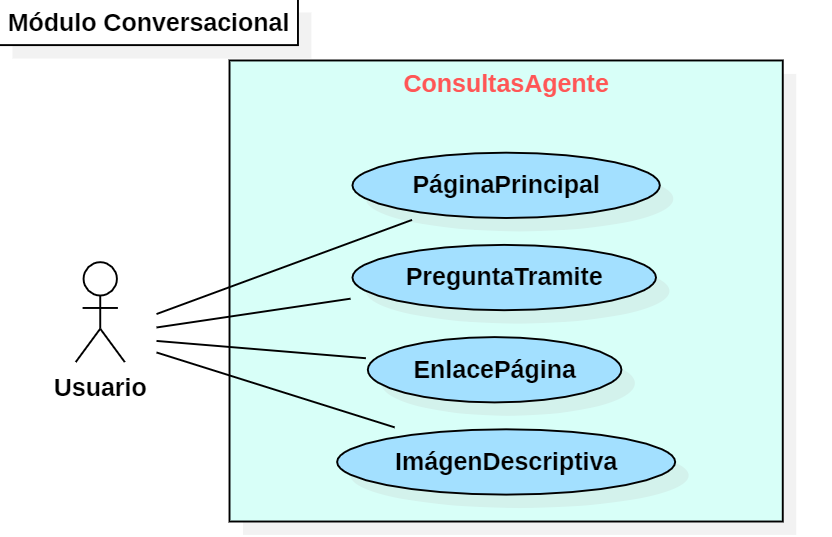
\includegraphics[width=0.7\textwidth]{figura3_5}
 \caption{Diagrama de casos de uso para la primera iteración.}
\label{fig:figura3_5}
\end{figure}

\subsection{ACTIVIDADES}
A continuación se definirá el proceso de flujo que seguirán los casos representados en la figura 3.5, se modelará la actividad de consulta de trámite, la interfaz conversacional mostrará una entrada donde el usuario deberá introducir su pregunta, se ofrecen dos vías de entrada que son escrita y por voz, luego de enviada la pregunta el sistema hará una petición HTTP de tipo POST enviando la pregunta a la API del sistema que usará servicios que retorne la respuesta del agente incluyendo los denominados payloads que serán envíos de tipo especial de respuesta además de texto como ser: imágenes, botones interactivos o mapas de Google. \par
En la figura 3.6, la actividad de consulta de trámite prepara la vista del módulo de Chat para interacción con usuario, esta clase define un método de entrada tipo texto que al abrirse carga un evento enviado denominado Saludo Inicial que cargará al cuerpo del chat un mensaje enviado por bot cada envío de algún mensaje realizado por un cliente seguirá el flujo de la consulta, una vez validado el mensaje se guardará en la base de datos mostrado en el modelo de contenido. 


\begin{figure}[H]
\centering
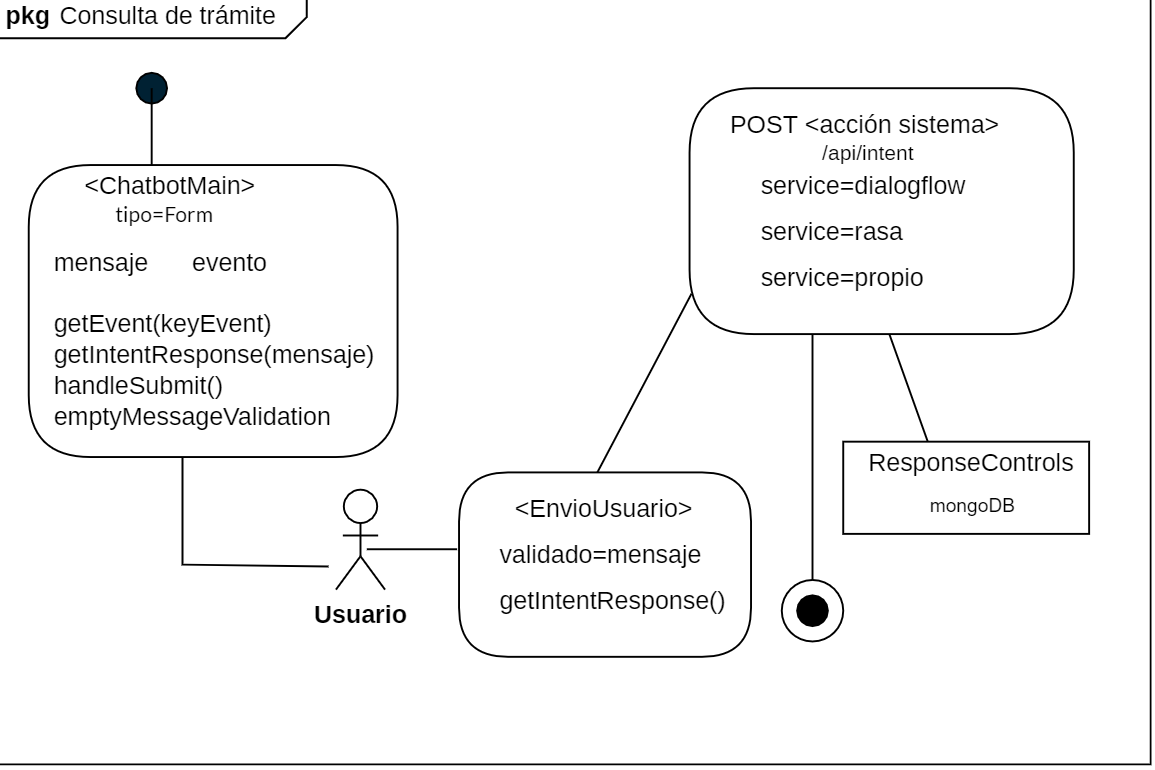
\includegraphics[width=0.8\textwidth]{figura3_6}
 \caption{Actividad Consulta Trámite.}
\label{fig:figura3_6}
\end{figure}





\par
Para la comunicación del agente conversacional y la interfaz de usuario no se puede hacer directamente debido a las credenciales de Dialogflow y también para comodidad de manejo de base de datos y la recolección de conversaciones, para esto se creará un microservicio API en Next para la comunicación y las rutas que se usarán. 
Con todo lo anterior la estructura del backend se muestra en la figura 3.7.

\begin{figure}[H]
\centering
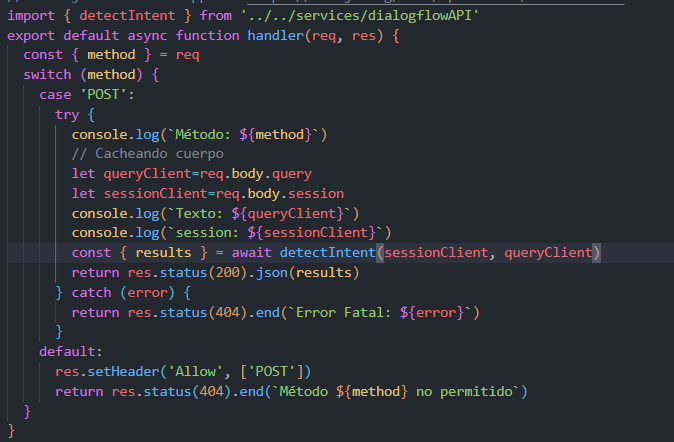
\includegraphics[width=0.6\textwidth]{figura3_7}
 \caption{Backend de comunicación con la interfaz y el agente.}
\label{fig:figura3_7}
\end{figure}

La implementación será detallada en ANEXO 1 donde se mostrarán las partes más importantes de código para la interacción entre las fases de comunicación de usuario y agente conversacional. Seguidamente se desarrolla una aplicación conversacional de forma de asistente virtual, esta forma de interacción es muy común y comercial en toda estructura conversacional de pregunta respuesta en una interacción de mensajes, respecto a las necesidades del proyecto este debe ser amigable y de interfaz conocida siguiendo una estructura típica entendible y manejable, una interfaz que sirve de inspiración tendrá la estructura parecida al siguiente ejemplo de maquetado como se muestra en la figura 3.8.

\begin{figure}[H]
\centering
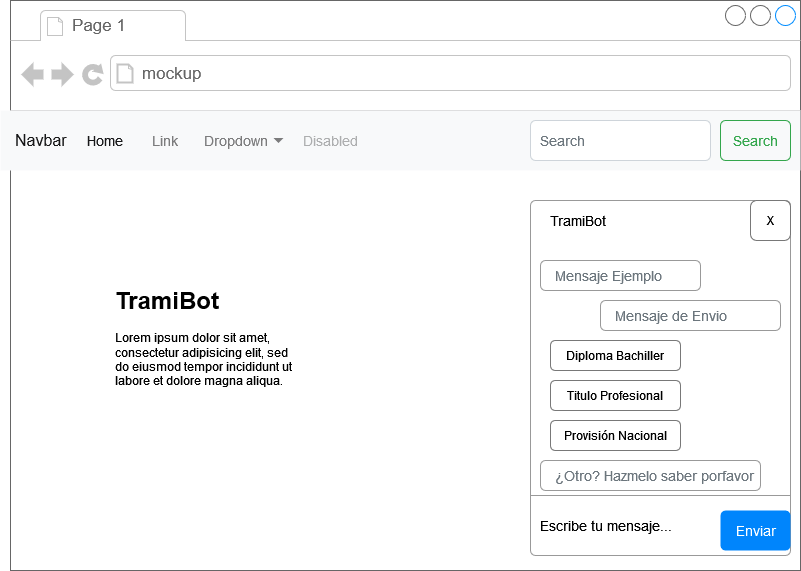
\includegraphics[width=0.7\textwidth]{figura3_8}
 \caption{Estructura de la interfaz de usuario pública.}
\label{fig:figura3_8}
\end{figure}

\subsection{MODELO DE CONTENIDO}
En la figura 3.9 se muestra el modelo estructurado para almacenar cada respuesta enviada por el agente, para gestión de administrador juzgando la efectividad a respuesta que tuvo el agente conversacional. 

\begin{figure}[H]
\centering
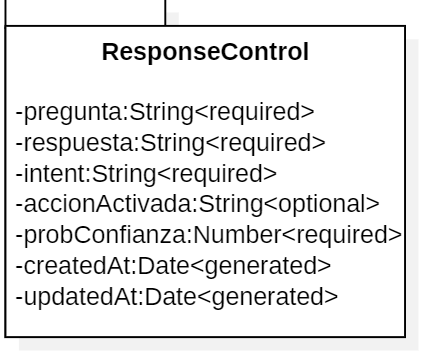
\includegraphics[width=0.3\textwidth]{figura3_9}
 \caption{Modelo de control de respuesta.}
\label{fig:figura3_9}
\end{figure}

\par En este sprint no se mostrará un modelo navegacional ya que será de tipo SPA por sus siglas en ingles que implican aplicación de una página debido a que no se presentará ninguna recarga de página para una experiencia de usuario más fluida. 

\subsection{MODELO DE PROCESO}

Debido a que será un módulo de chat estático el proceso es muy simple se mostrará en la figura 3.10 el diagrama de secuencia de la interacción de la primera interacción que tiene el agente conversacional con el usuario. 

\begin{figure}[H]
\centering
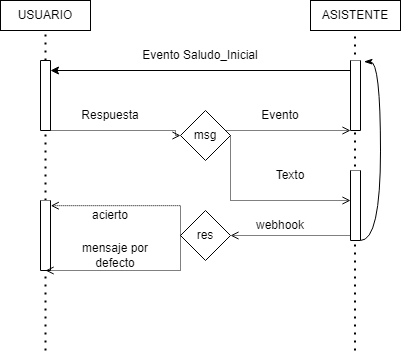
\includegraphics[width=0.5\textwidth]{figura3_10}
 \caption{Diagrama de secuencia primera iteración apretura conversacional}
\label{fig:figura3_10}
\end{figure}

La figura 3.10 muestra la forma en el que el usuario podrá conversar con el agente, al principio siempre se iniciará el diálogo por el agente ofreciéndole alternativas a preguntas que podrían interesarle al usuario, luego el usuario puede pedirle al agente iniciar una conversación con alguna de las alternativas o introducir texto o audio por la interfaz, esto hará que el servicio de conversación como dialogflow trate de predecir si se puede relacionar a la pregunta con alguna intención con palabras de entrenamiento que se realizó previamente.
\par
Si logra superar el umbral de aceptación se envía al usuario una respuesta predefinida o se manda una solicitud de información a un servicio de webhook definido por rutas definidas en el servidor desarrollado, esta etapa de desarrollo deberá tener una base de datos relacional que envíe datos como el horario de apertura de algún punto de información y recepción de documentos, o los costos, las páginas donde se puede obtener más información, entre otros.

\subsection{MODELO DE PRESENTACIÓN}

El desarrollo del marco de desarrollo NextJS permite hacer uso de rutas dinámicas a diferencia de la librería React, como esta será una aplicación amplia se requiere apoyarse en un marco de trabajo basado en React, en esta primera iteración se muestra la navegación básica que tendrá la vista. 


\begin{figure}[H]
\centering
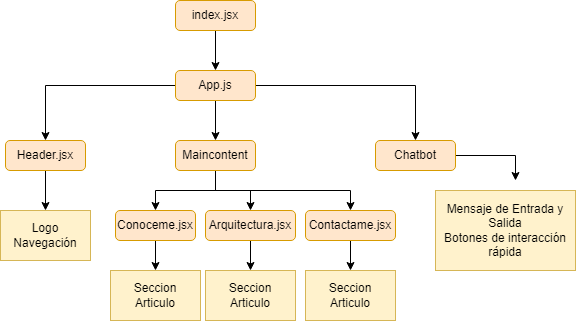
\includegraphics[width=0.6\textwidth]{figura3_11}
 \caption{Componentes desarrollados en la fase inicial de desarrollo de interfaz de usuario}
\label{fig:figura3_11}
\end{figure}

Desarrollando esta iteración en la figura 3.12 se consigue el siguiente resultado estático previo, usando {\it tailwind} para acortar el tiempo de desarrollo de {\it frontend}. Tomando inspiración de otros asistentes virtuales comerciales se tendrá un botón de acceso al asistente virtual para consultas al lado derecho y debajo de la pantalla del usuario, al presionar se desplegará el componente conversacional, que en el montaje inicial hará su primera comunicación con el agente virtual con la consulta de bienvenido, específicamente desarrollado para la intención de respuesta de primera comunicación con el usuario. 
\par

\begin{figure}[H]
\centering
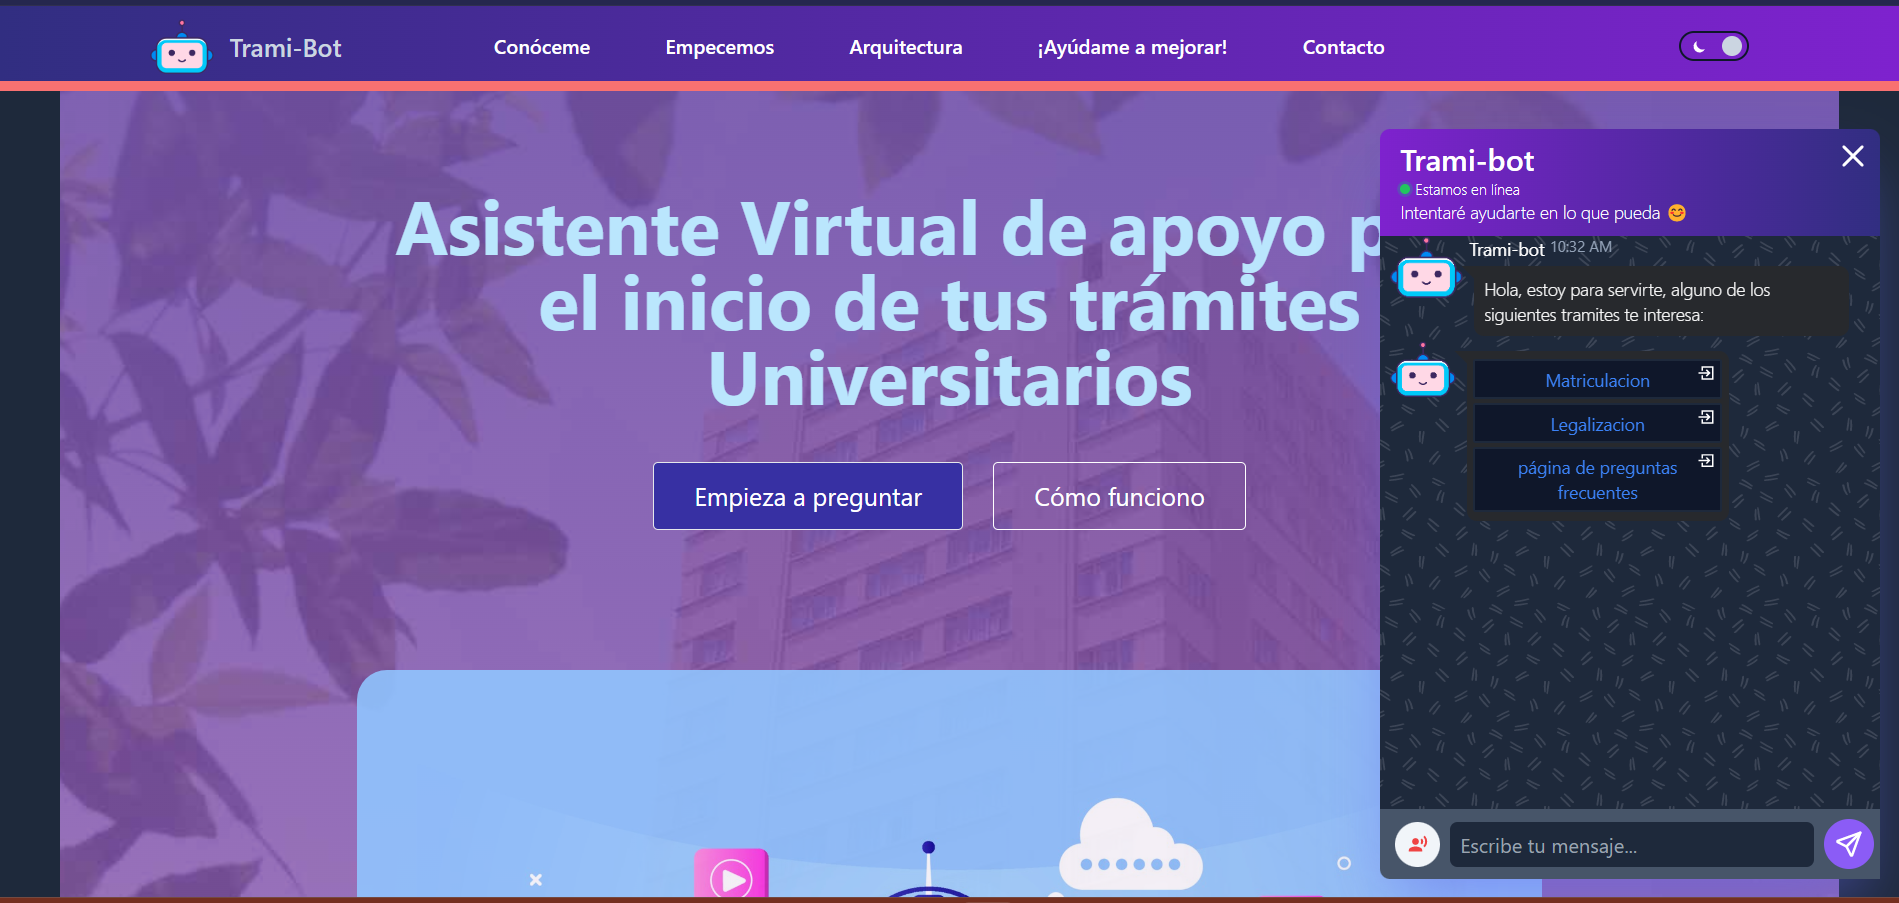
\includegraphics[width=0.7\textwidth]{figura3_12}
 \caption{Resultado de la primera estructura de la interfaz de usuario usando el marco de trabajo NextJS}
\label{fig:figura3_12}
\end{figure}

La respuesta enviada por el agente conversacional contendrá tanto la respuesta implementada en el agente como la confianza de clasificación de la intención, la colección de respuestas, el contexto, los parámetros que habría encontrado y demás detalles usados posteriormente para la construcción de los flujos conversacionales. 
Después de verificar la comunicación entre API’s se puede hacer la comunicación entre la parte del cliente con el servidor haciendo peticiones en la ruta correspondiente. 
\par
En la figura 3.12 se muestra como se construyen los botones interactivos como funcionalidad adicional para el tramibot, además el agregado de escritura de mensaje por voz y el modo día y noche que es muy común en las aplicaciones web actuales. 

\begin{figure}[H]
\centering
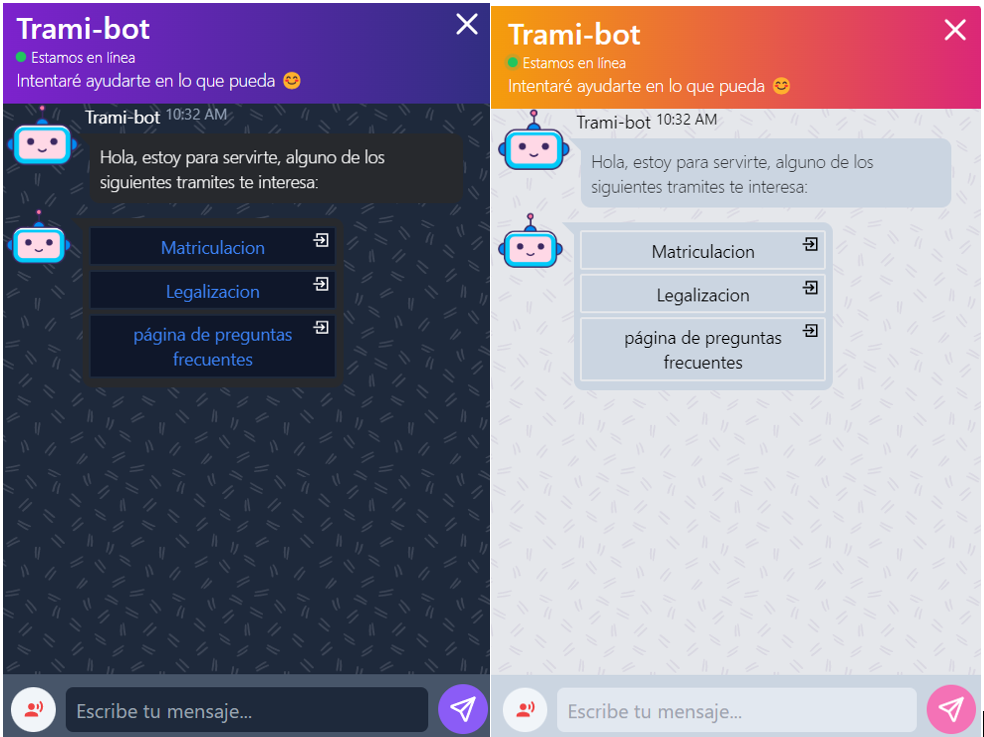
\includegraphics[width=0.4\textwidth]{figura3_13}
 \caption{Comunicación con la interfaz del cliente modo día y noche con las respuestas rápidas implementadas mediante uso de {\it payload}}
\label{fig:figura3_13}
\end{figure}


\section{SEGUNDA ITERACIÓN}
Para la segunda iteración se planea construir un constructor de flujos de conversación de manera gráfica y sencilla de implementar, esta alternativa no se ofrece en las versiones gratuitas tanto de {\it rasa} y {\it dialogflow es}; ambos servicios poseen un servicio más óptimo en este tipo de construcciones, estas alternativas de pago se llaman {\it rasax} y {\it dialogflow cx} que como ventaja ofrecen vistas interactivas para la construcción de conversaciones con contexto.
\par
Se define un sprint backlog teniendo en cuenta todo lo que se necesita para construir una aplicación web en su faceta administrativa: sean los registros e ingresos de los usuarios, implementando el uso de {\it tokens} las rutas mínimas necesarias para la gestión de administración y las rutas necesarias para la construcción de estos circuitos conversacionales de manera visual. 

\begin{table}[H]
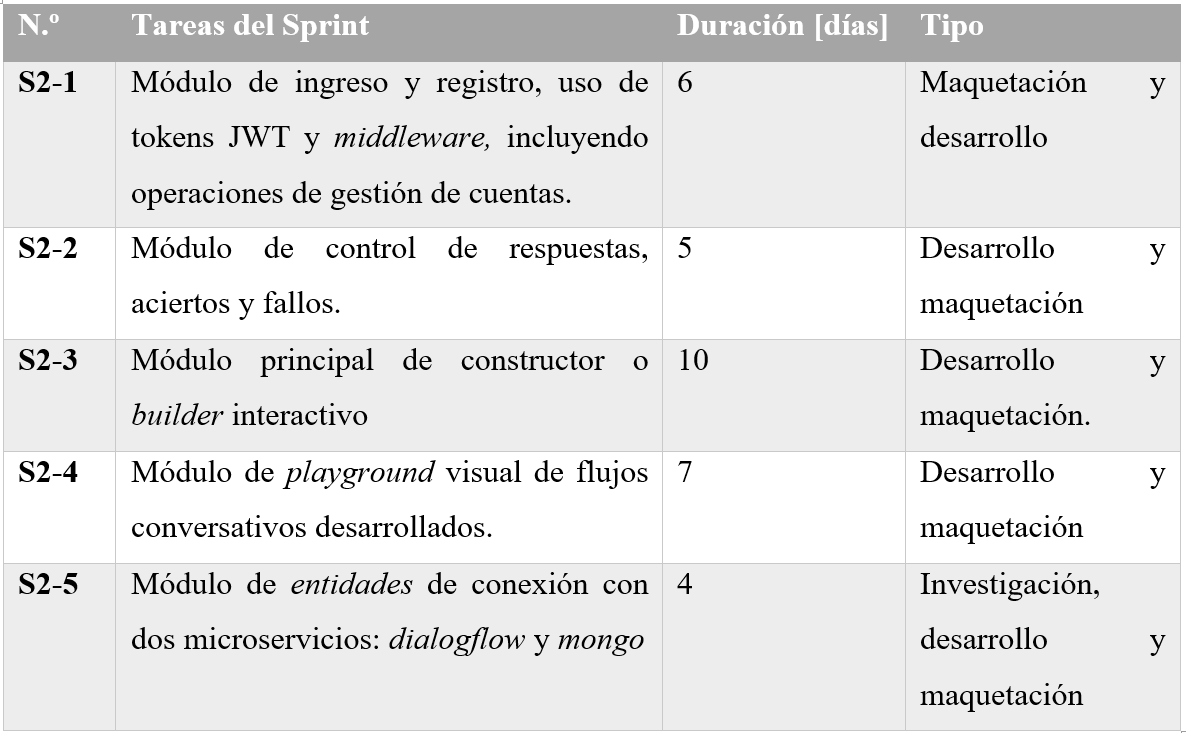
\includegraphics[width=1\textwidth]{tabla3_9}
\caption{Construcción del {\it sprint backlog} para la segunda iteración. } 
\label{tab:tabla3_9} 
\end{table}

En la tabla 3.9 se muestran todas los {\it sprints} necesarios para construir un sistema completo de un agente conversacional basado en microservicios, en la primera iteración se notaron las flaquezas de lado del desarrollo al tener que hacer uso de una interfaz gráfica de creación de conversaciones en el servicio gratuito de {\it dialogflow es}; dado que se pretende tener control y almacenar todas las interacciones se considera la historia de usuario de rol de administrador en alto y se crean todos estos tipos de experiencia de usuario respectiva al acceso de un sistema. 

\subsection{MODELO DE REQUERIMIENTOS}

Considerando la misma estructura de la primera iteración a continuación se mostrarán los casos de uso que se tomarán en cuenta para este ciclo de desarrollo. 

\begin{figure}[H]
\centering
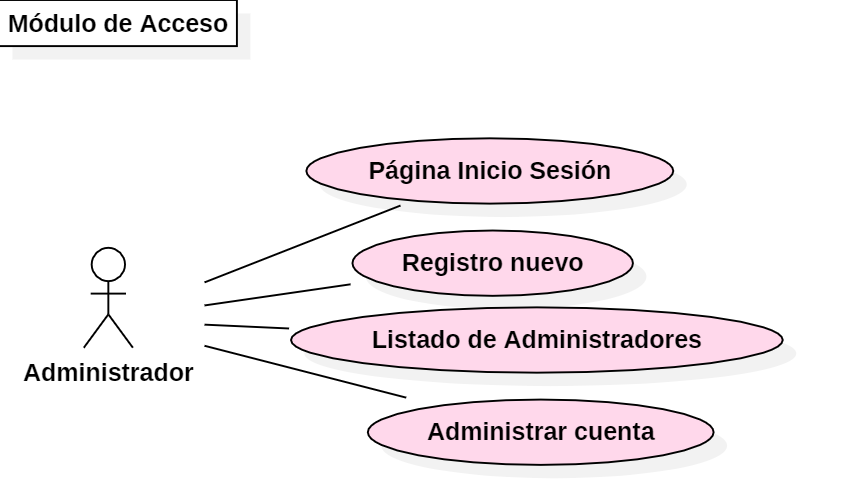
\includegraphics[width=0.6\textwidth]{figura3_14}
 \caption{Caso de uso acceso a administrador}
\label{fig:figura3_14}
\end{figure}

En la figura 3.14 se considera el módulo de administrador, señalando las interacciones que tendrá un administrador desde que ingresa al sistema y todo el control que pueda tener en este {\it sprint}. 
\par En la figura 3.15 se define los casos de uso del módulo de control de respuestas, aciertos y fallos. 

\begin{figure}[H]
\centering
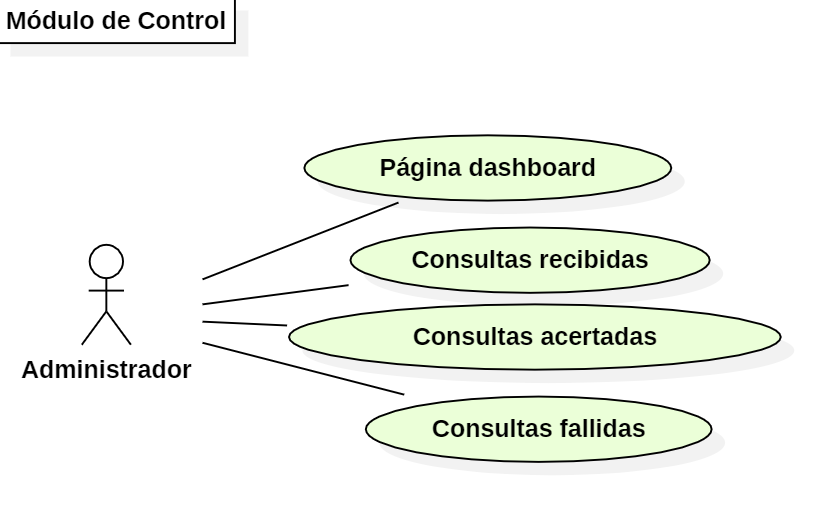
\includegraphics[width=0.6\textwidth]{figura3_15}
 \caption{Caso de uso control de respuestas, aciertos y fallos}
\label{fig:figura3_15}
\end{figure}

La figura 3.16 se considerará unir los {\it sprint's} de {\it builder} y {\it playground}; junto con el módulo de entidades descrito a continuación se muestran los casos de uso que se tendrán en todas esas interacciones. 

\begin{figure}[H]
\centering
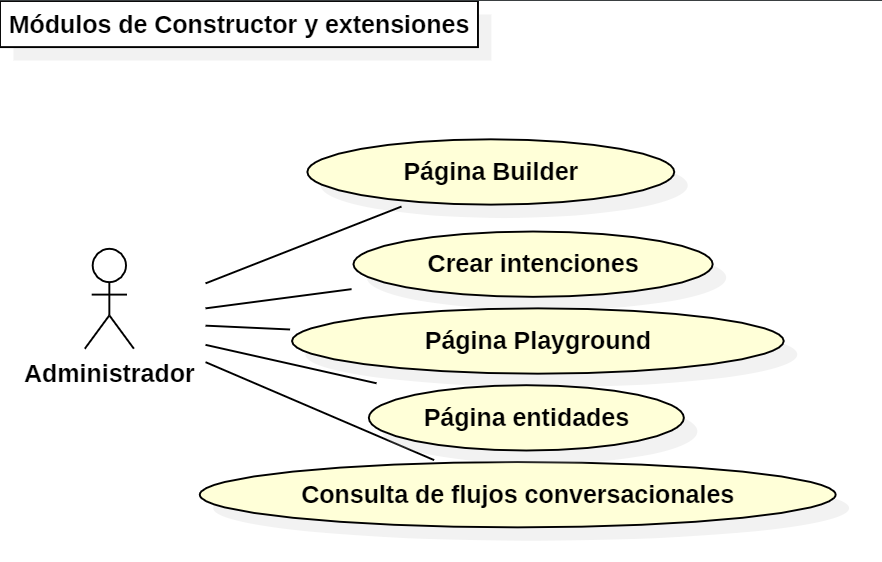
\includegraphics[width=0.5\textwidth]{figura3_16}
 \caption{Caso de uso {\it builder} y {\it playground} más extensiones}
\label{fig:figura3_16}
\end{figure}

\subsection{ACTIVIDADES}

Cada caso en los requermientos presentados tendra un proceso que seguirán para mostrar los dos casos que se consideran raíces a cada {\it sprint } se considera la página {\it builder}, se detallarán algunos procesos en ANEXO 2.

\begin{figure}[H]
\centering
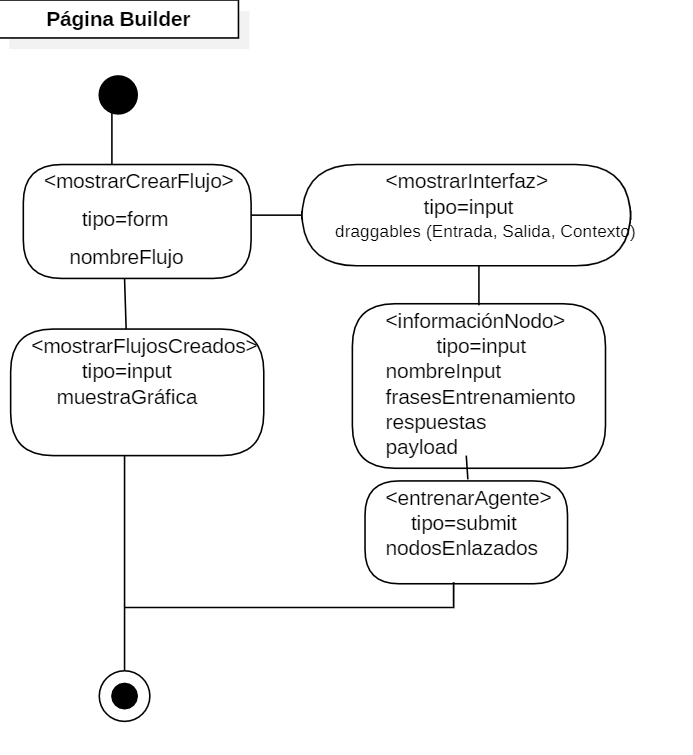
\includegraphics[width=0.5\textwidth]{figura3_17}
 \caption{Actividad desarrollada en la construcción de un flujo conversacional. }
\label{fig:figura3_17}
\end{figure}

En la figura 3.17 se considera la actividad que se desarrollará en el módulo de construcción de circuitos conversacionales, ofreciendo la alternativa de visualizar los modelos previos desarrollados de manera visual, con la información de cada nodo correspondiente a un mismo contexto. 
Los demás casos se mostrarán en el modelo de presentación donde se explicará más detalladamente como se implementaron las distintos modulos completos. 

\subsection{MODELO DE CONTENIDO}
Para poder almacenar la información de cada usuario se guardará usando el servicio de {\it MongoDB} desarrollando el modelo de la figura 3.18 que corresponde a administradores. 

\begin{figure}[H]
\centering
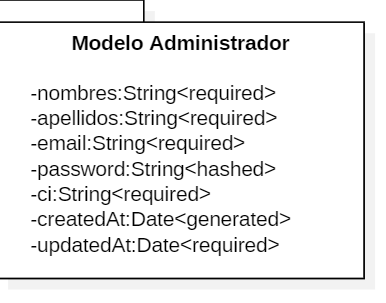
\includegraphics[width=0.3\textwidth]{figura3_18}
 \caption{Modelo de administradores en la base de datos. }
\label{fig:figura3_18}
\end{figure}

El siguiente modelo será el de {\it flows } que almacenará todos los circuitos conversacionales para su despliegue y uso posterior, teniendo dos estructuras que son los nodos y {\it edges}, cada nodo almacenará la información de cada intención entrenada en el agente; haciendo uso de la base de datos para no realizar peticiones que no sean entrenamiento o predicción al servicio. La figura 3.19 muestra la representación gráfica del módulo {\it builder}. 

\begin{figure}[H]
\centering
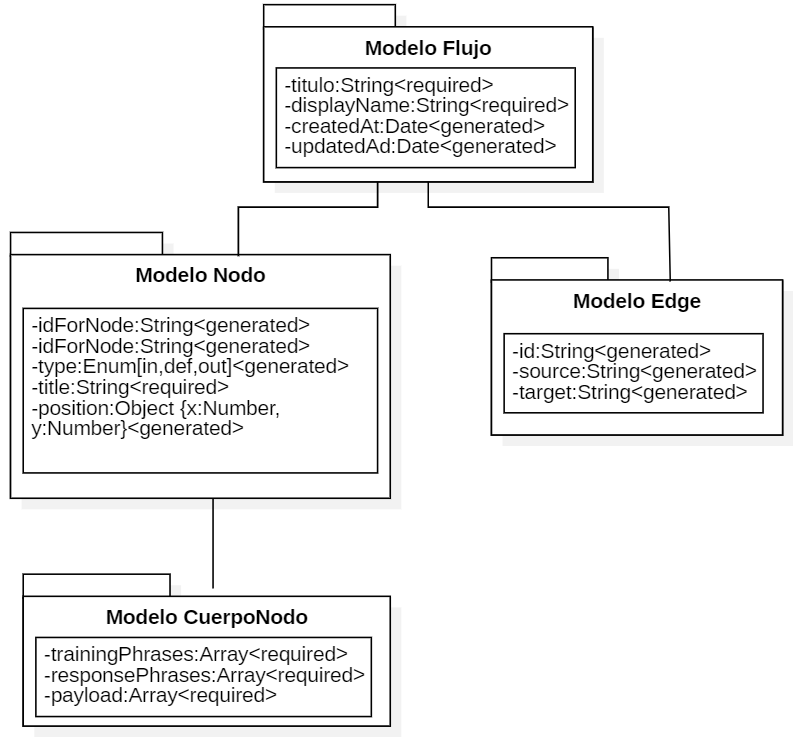
\includegraphics[width=0.7\textwidth]{figura3_19}
 \caption{Modelo de constructor de circuitos de conversación. }
\label{fig:figura3_19}
\end{figure}

\subsection{MODELO DE PROCESO Y PRESENTACIÓN}

Esta sección será un detalle de las consideraciones al construir cada módulo de el {\it sprint}. Lo principal a considerar en un módulo de sesión es el uso de un sistema de seguridad ya sea por sesión o por token, la aplicación se implementa con el uso de un token único por sesión de 30 días, JWT o { \it o json web token} es un estándar para la creación de datos con firma o encriptación, el cual contiene información representada en formato JSON, considerado como una alternativa segura para un módulo de sesiones. Se hará uso de una implementación del token y un {\it middleware } que verifique el token único, considerado una autenticación desde servidor, como muestra la figura 3.20. sigue el proceso de autenticación tanto de inicio de sesión como de registro. 


\begin{figure}[H]
\centering
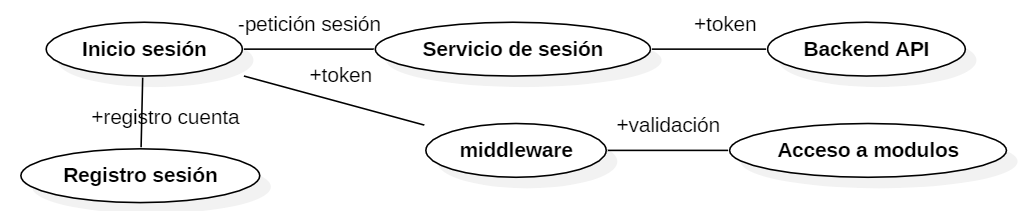
\includegraphics[width=0.9\textwidth]{figura3_20}
 \caption{Proceso de registro e inicio de sesión por medio de {\it token}. }
\label{fig:figura3_20}
\end{figure}

Se procedió a desarrollar una interfaz gráfica tanto de inicio de sesión como de registro de nuevo usuario, con validadores de entrada tanto en cliente con {\it live validators} y en servidor con {\it helpers}. La figura 3.21 muestra la presentación de las páginas de registro e inicio de sesión, así también las operaciones del control de cuentas de administradores. 


\begin{figure}[H]
\centering
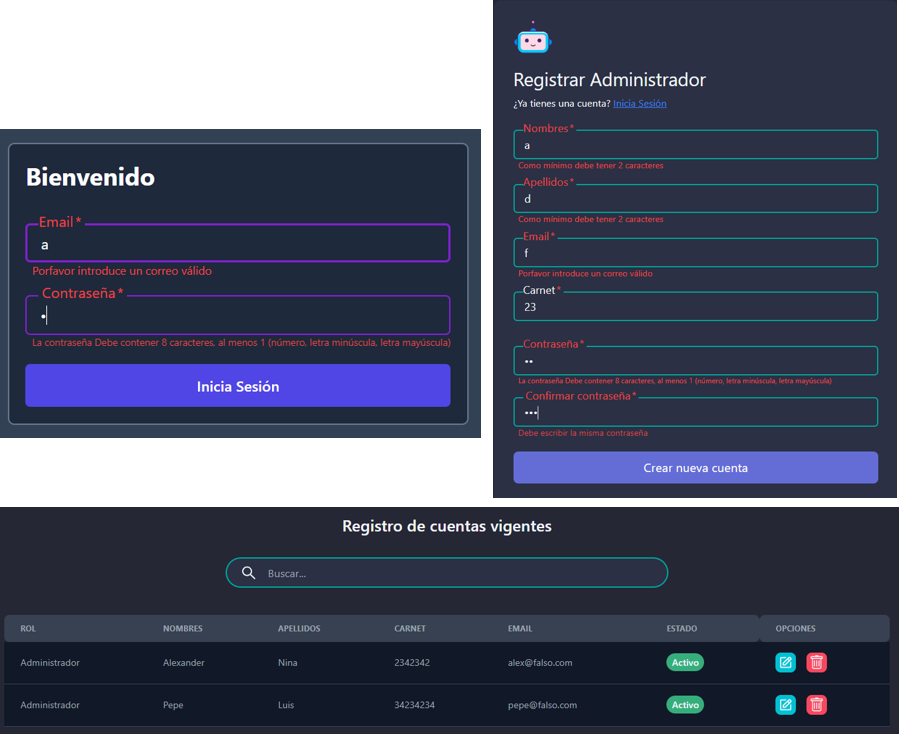
\includegraphics[width=0.5\textwidth]{figura3_21}
 \caption{Páginas de registro e inicio de sesión. }
\label{fig:figura3_21}
\end{figure}


De la misma manera se mostrará los procesos implementados en el constructor que servirá como base para previos diseños, tomando en cuenta la figura 3.17 se implementará una interfaz con la estructura mencionada basada en estados por tiempo de uso se estructuran la petición de {\it flows} a la base de datos o la creación de una nueva estructura para su entrenamiento posterior. La figura 3.22 muestra el estado inicial que tendrá la ruta {\it builder}. 

\begin{figure}[H]
\centering
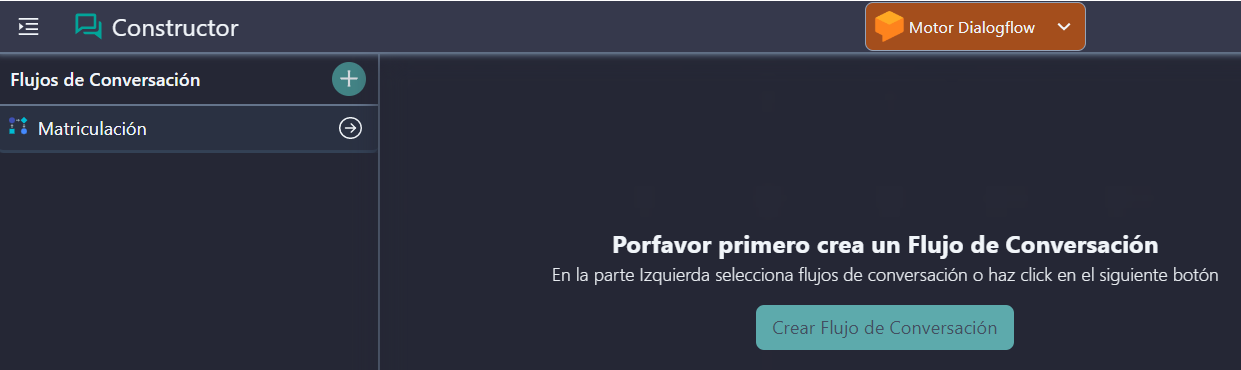
\includegraphics[width=0.8\textwidth]{figura3_22}
 \caption{Estado principal página de constructor. }
\label{fig:figura3_22}
\end{figure}

Después de seleccionado el nombre que tendrá un circuito conversacional se presentará una interfaz un poco más estructurada, con los nodos, que guardarn opciones como frases de entrenamiento y respuesta. Estos nodos se almacenarán y entrenarán el agente de forma posterior. En la figura 3.23 se muestra el diseño que se desarrollo para la implementación de este módulo. 


\begin{figure}[H]
\centering
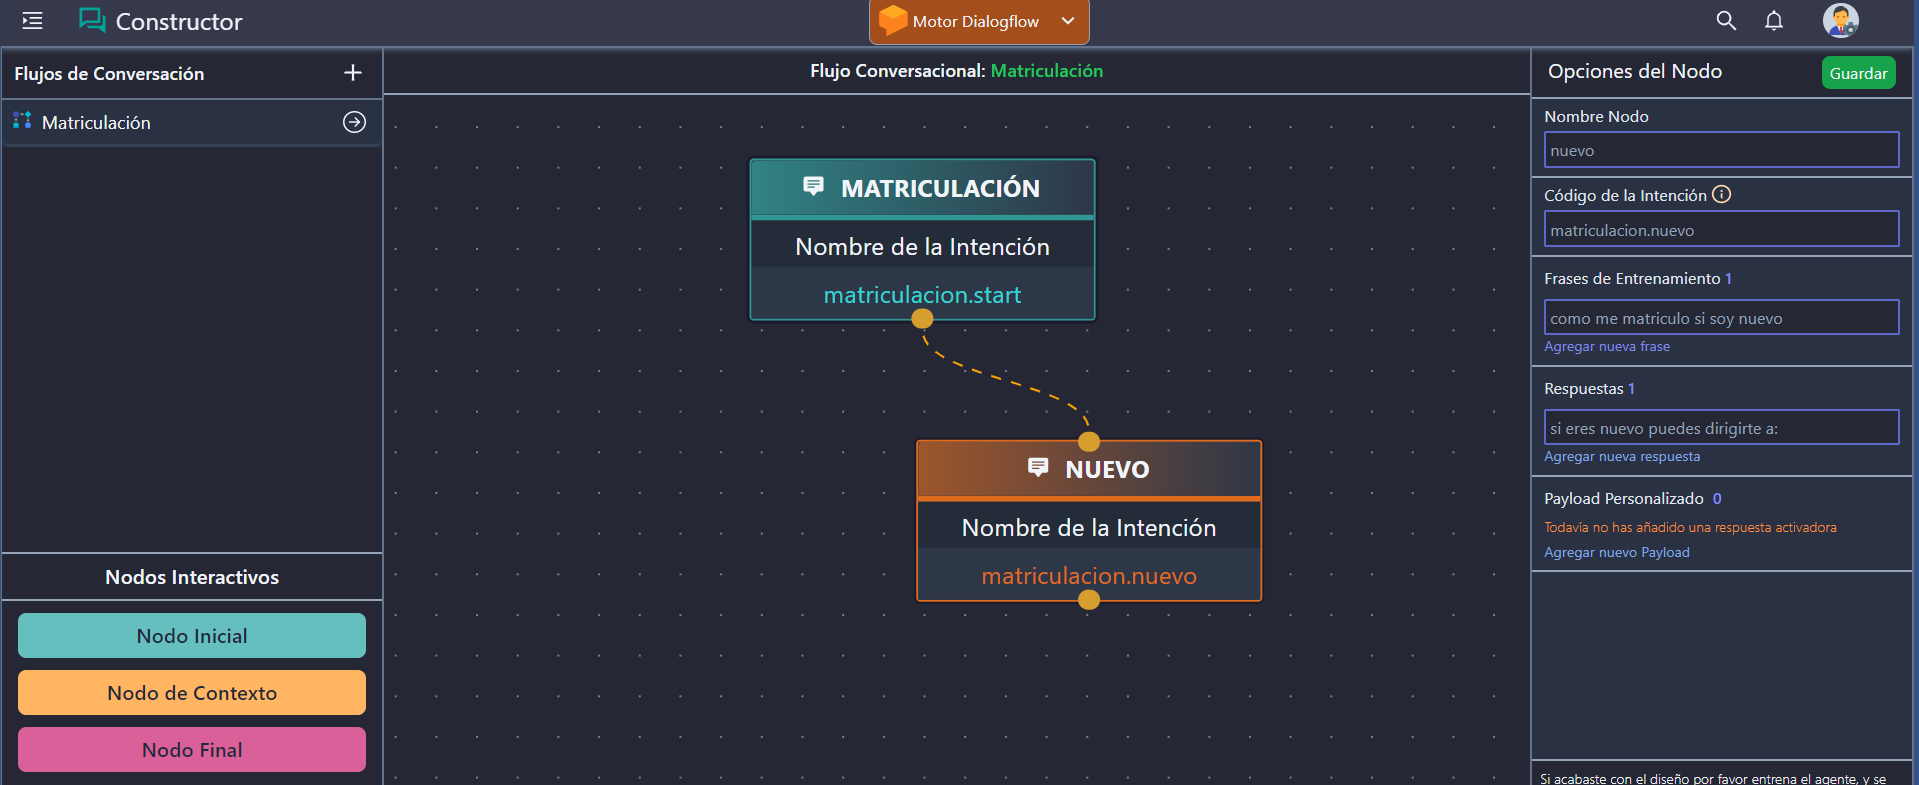
\includegraphics[width=0.8\textwidth]{figura3_23}
 \caption{Estado de construcción circuito de conversación. }
\label{fig:figura3_23}
\end{figure}

Otro estado que puede tener el constructor el la visualización de flujos ya desarrollados y estructurados, en el motor de navegación denominado {\it playground} se implementó un módulo de conversación y los flujos ya desarrollados también como se muestra en la imágen, esto para poder poner en práctica la funcionalidad o falla de las construcciones que se vayan desarrollando. La figura 3.24 muestra como fue implementado el módulo de {\it playground}.


\begin{figure}[H]
\centering
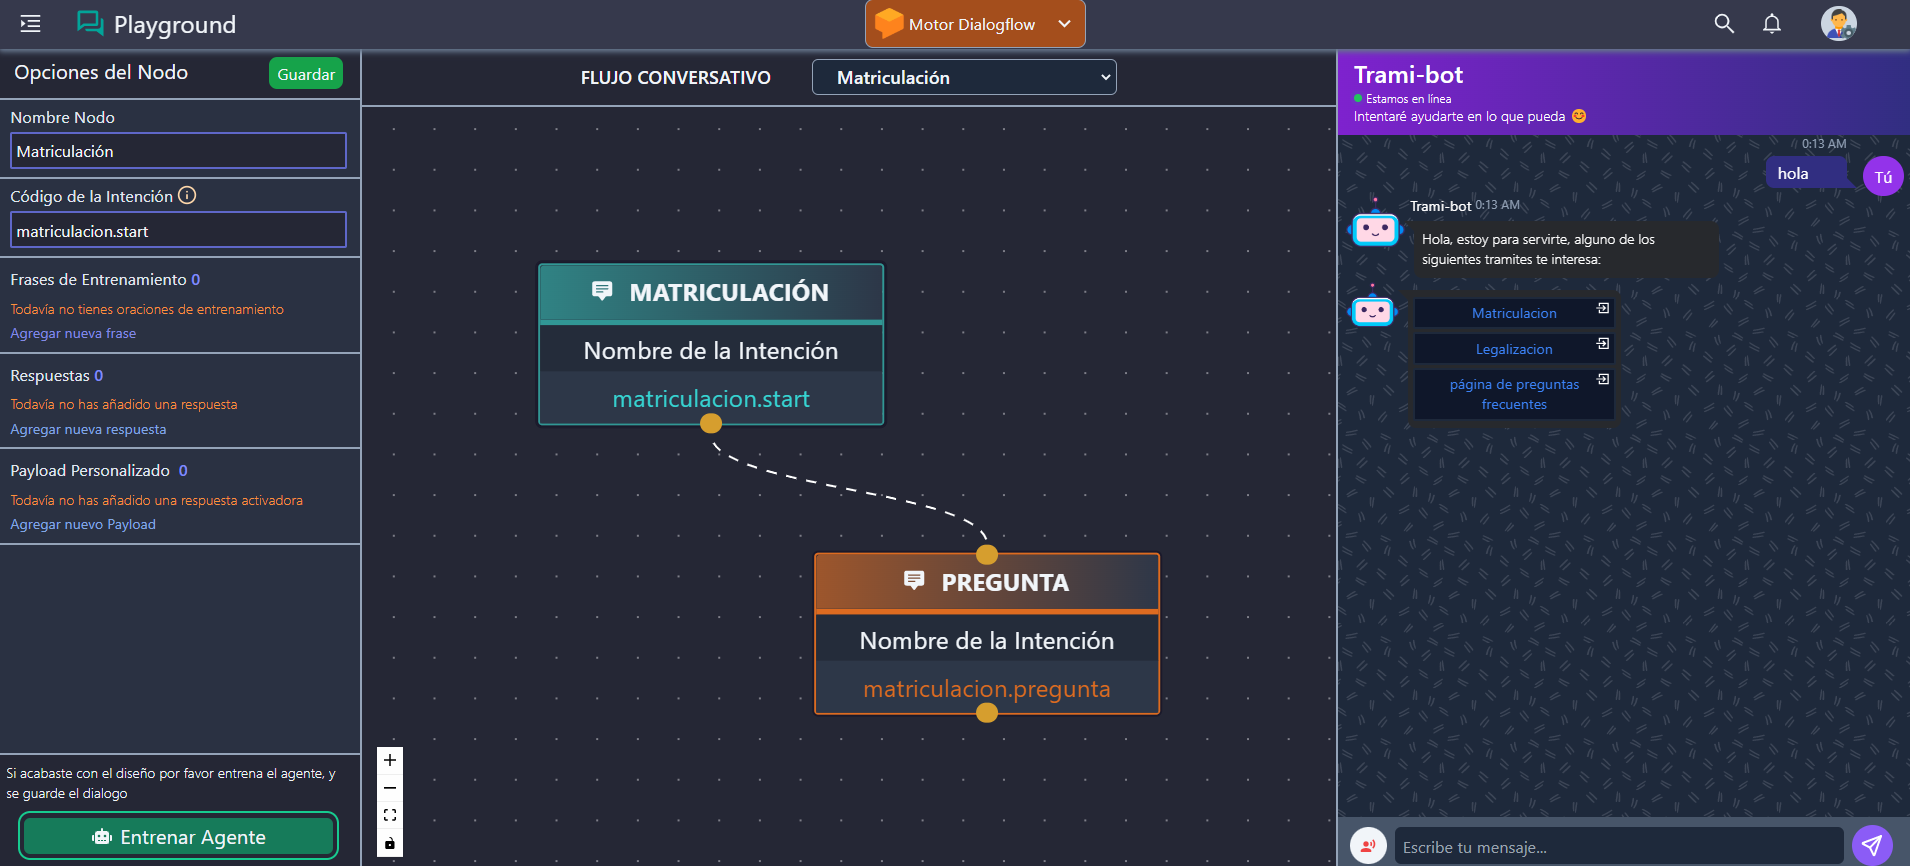
\includegraphics[width=1\textwidth]{figura3_24}
 \caption{Módulo {\it playground} en un estado de prueba en interfaz de cliente.  }
\label{fig:figura3_24}
\end{figure}

Como se describió en la figura 3.23 cada nodo tendrá una información diferenciada con respecto a otro; además de una respuesta textual que el agente puede responder, se puede mandar datos específicos como imágenes, enlaces a páginas informativas o {\it events}; este último siendo un activador sin realizar consulta de alguna intención en particular. La figura 3.25 muestra que el sistema puede alojar imágenes de apoyo que el administrador desee para que el agente pueda mostrar la ubicación física de algún punto importante donde se realice algún trámite o consulta de información. 

\begin{figure}[H]
\centering
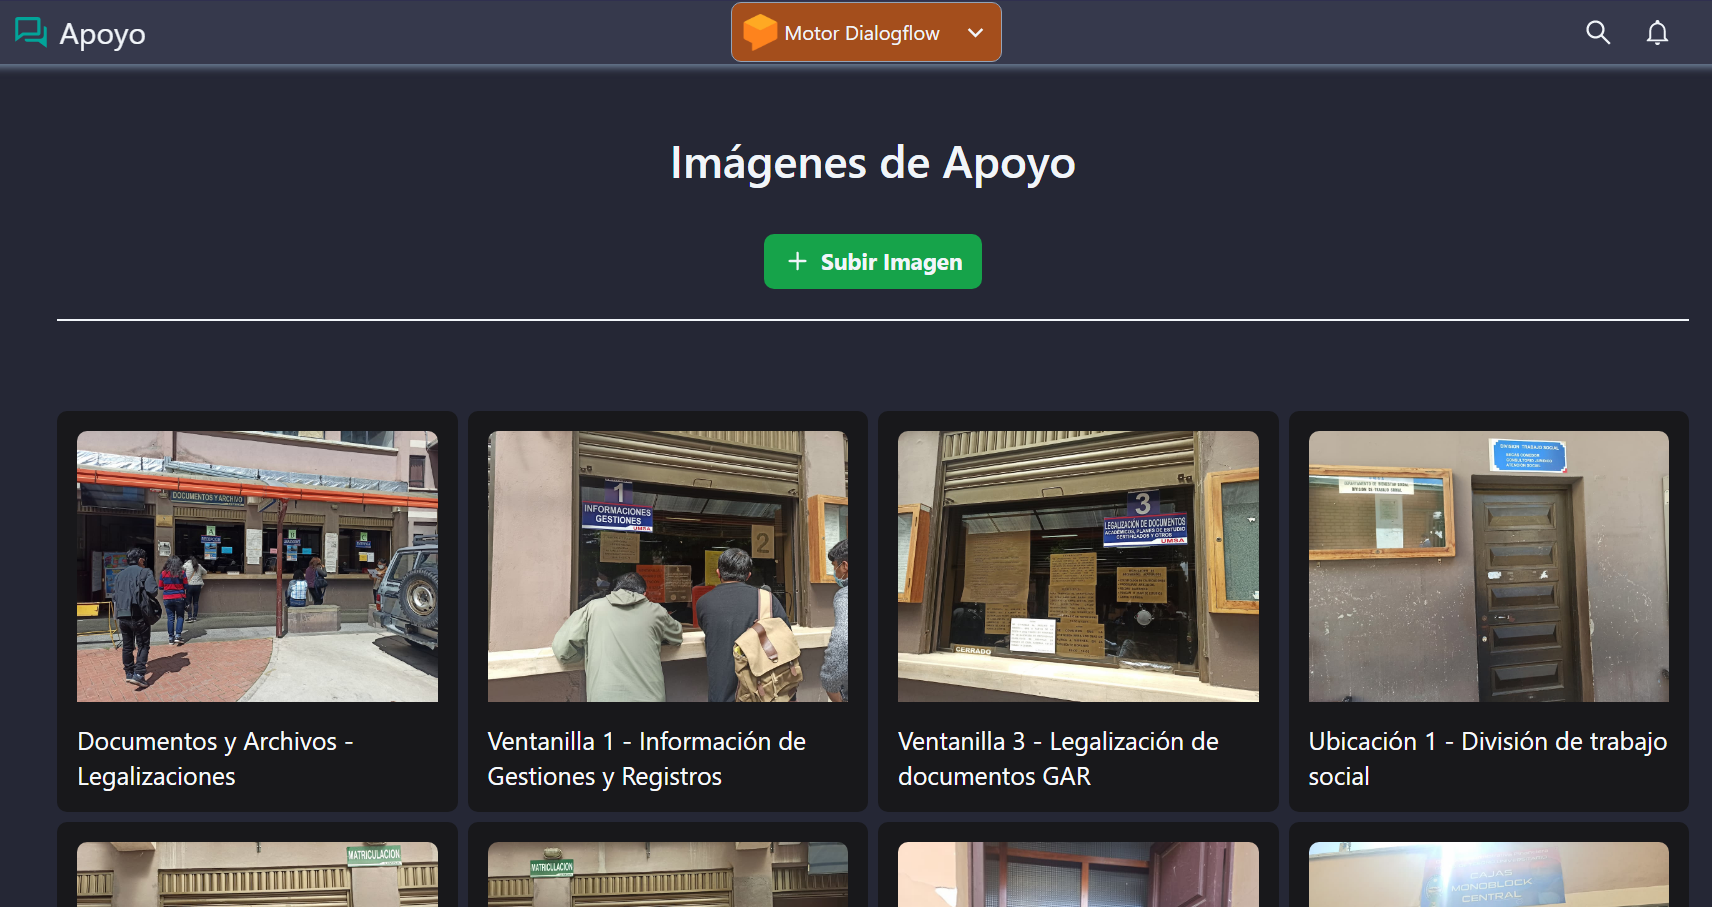
\includegraphics[width=0.8\textwidth]{figura3_25}
 \caption{Módulo imágenes de apoyo alojado en {\it cloudinary}.  }
\label{fig:figura3_25}
\end{figure}

\section{TERCERA ITERACIÓN}

Esta tercera iteración será el inicio de la creación de varios circuitos conversacionales independientes, la ventaja que tiene el sistema es simular circuitos que un usuario pueda seguir, en el servicio de {\it dialogflow} se denominan a estas estructuras flujos y en {\it rasa} son historias, teniendo estos circuitos bien definidos pueden ser capaces de ser generalizados a conversaciones nunca antes vistas. 
\par 
Para las siguientes iteraciones se cambiará de metodología haciendo uso de la metodología IMADTC (metodología iterativa para el análisis y desarrollo de {\it chatbots} textuales), a continuación se describirá la estructura  propuesta por la metodología y se tratará de enfocar lo mejor posible a este caso. 
\begin{enumerate}
\item Contextualización del dominio del {\it chatbot}
\item Ejecución cíclica de los pasos:
	\begin{itemize}
	\item Preparación de objetivos
	\item Diseño de escenarios
	\item Diseño de flujo conversacional
	\item Prototipo
	\item Test de Usuario
	\item Documentación
	\end{itemize}
\end{enumerate}

\par Ccomo respuesta al segmento secuencial de contextualización del dominio se presentan las siguientes consideraciones.
{\begin{itemize}
\item {\textbf{¿Para qué propósito está desarrollando el {\it chatbot} como sistema?} El presente agente conversacional basado en objetivos tiene como propósito de ser informativo, lo que significa que no pedirá información de tipo personal, como ser datos de registro universitario; no se cuenta con esa información personalizada. El objetivo principal es brindar información sobre lugares, procedimiento e información de páginas correspondientes de algún tipo de trámite. } 

\item {\textbf{¿Bajo que rol opera el {\it chatbot}?} El rol del {\it chatbot} pertenece al apoyo informativo o atención al cliente, carente de personalidad específica basado en respuestas dadas por el administrador. }
 
\item {\textbf{¿Va a interaccionar con otros sistemas {\it software}?} Al trabajar con una arquitectura basada en microservicios el agente no trabajará solo con el servicio de {\it dialogflow}, sino que se integrará el {\it dataset} construido por este servicio con otros como: {\it rasa} y uno propio basado en redes neuronales, para posible estudio de casos a posterior.}
 
\item {\textbf{¿Qué es lo que el {\it chatbot} no debe hacer explícitamente?} El sistema conversacional no considera el uso de {\it fullfillments} o {\it actions}, debido a que no trabaja con datos privados correspondientes a cada facultad y su carrera correspondiente. Tampoco se considera tratar temas más específicos como: record académico, plan de estudios, etc. Siendo información bastante particularizada que mi persona no tiene acceso. } 

\end{itemize}

\par
con la definición clara de las características del {\it chatbot} se procederá a definir iteraciones de flujos independientes. 

\subsection{FLUJO DE CONVERSACIÓN CARRERA PARALELA}
Como un circuito diferenciado se tomará como primer estructura una carrera paralela, que es un trámite muy común a realizar por la comunidad estudiantil; se tomarán en cuenta aspectos informativos para responder a las preguntas más generales que un estudiante se haría sobre este proceso. 

\begin{enumerate}[label=(\alph*)]
	\item \textbf{Selección de objetivos}
	\par Para realizar esta fase se pueden volver a tomar las historias de usuario en una forma más específica pero podemos definir textualmente cuales serían las dudas más generales sobre este proceso: lugar de información, tabla de valores, procedimiento a seguir, página de más información y otras alternativas interesantes para el cliente. 
	
	\item \textbf{Diseño de escenarios}
	\par Definido a grandes rasgos se tomará como ejemplo al lugar físico de información, los recursos necesarios definidos será la información recaudada usando la técnica de la entrevista descrita al inicio del capítulo.
	
	\item \textbf{Diseño de flujo conversacional}
	
	\par La figura 3.26 presenta a continuación los diagramas de flujo conversacional del resultado de los escenarios específicados. 
	\begin{figure}[H]
\centering
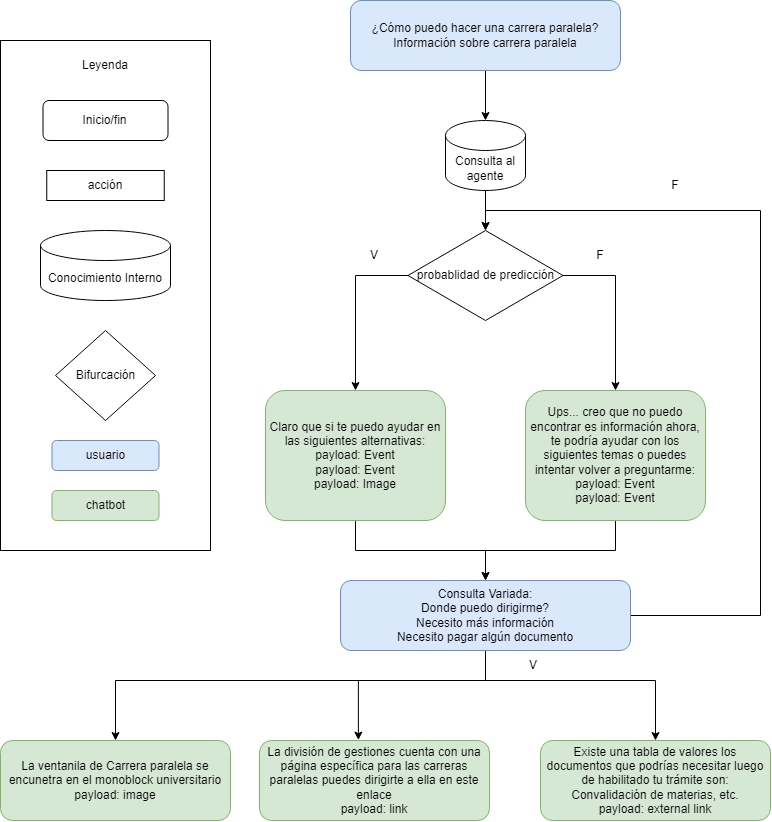
\includegraphics[width=1\textwidth]{figura3_26}
 \caption{Circuito conversacional carrera paralela.  }
\label{fig:figura3_26}
\end{figure}
	
	\item \textbf{Desarrollo del prototipo}
	\par A continuación la figura 3.26 muestra la implementación en la interfaz gráfica desarrollada todo el circuito gráfico
	\begin{figure}[H]
\centering
\includegraphics[width=0.8\textwidth]{figura3_27}
 \caption{Circuito conversacional físico almacenado en base de datos y servicios de conversación - carrera paralela.  }
\label{fig:figura3_27}
\end{figure}

\item \textbf{Test del circuito}
\par Para poder probar si esta en funcionamiento el circuito conversacional se deberá probar en la ruta de {\it playground} la figura 3.28 muestra como se va probando la funcionalidad del circuito.
	\begin{figure}[H]
\centering
\includegraphics[width=0.9\textwidth]{figura3_28}
 \caption{Pruebas iniciales del circuito implementado para carrera paralela.  }
\label{fig:figura3_28}
\end{figure}


\end{enumerate}

\subsection{FLUJO DE CONVERSACIÓN APOSTILLA}

\begin{enumerate}[label=(\alph*)]
	\item \textbf{Selección de objetivos}
	\par Tomando en cuenta la información general, solicitud de apostillado, seguimiento de la apostilla, el método de realización de pago, los puntos de atención y páginas de información relacionados al trámite de apostillado se ocnsidera el escenario definido a continuación.  
	
	\item \textbf{Diseño de escenarios}
	\par Descritos como videos tutoriales, páginas de información en la división de títulos y diplomas; y en la página de ministerio de relaciones exteriores se puede realizar la apostilla.
	
	\item \textbf{Diseño de flujo conversacional}
	
	\par La figura 3.29 presenta a continuación los diagramas de flujo conversacional del resultado de los escenarios específicados. 
	\begin{figure}[H]
\centering
\includegraphics[width=0.7\textwidth]{figura3_29}
 \caption{Circuito conversacional apostilla.  }
\label{fig:figura3_29}
\end{figure}
	
	\item \textbf{Desarrollo del prototipo}
	\par A continuación la figura 3.30 muestra la implementación en la interfaz gráfica desarrollada todo el circuito gráfico
	\begin{figure}[H]
\centering
\includegraphics[width=0.6\textwidth]{figura3_30}
 \caption{Circuito conversacional físico almacenado en base de datos y servicios de conversación - apostilla.  }
\label{fig:figura3_30}
\end{figure}

\end{enumerate}

\subsection{CUARTA ITERACIÓN}

Cómo se definieron en la tercera iteración se procede a dearrollar de forma contína la implementación y mejora de los circuitos siguiendo la investigación desarrollada en la sección 2.8 y sus trámites relacionados. 

\chapter{RESULTADOS}

En este capítulo se considera el \textit{software testing}, orientado a verificar y validar la calidad del \textit{software} y considerando los límites y fallas que pueda tener el sistema, tradicionalmente las técnicas orientadas a la prueba de software se pueden clasificar en las técnicas de caja blanca y caja negra; llamadas también prueba funcional y prueba estructural. Se considera que es esencial cubrir ambas técnicas 

\section{PRUEBA ESTRUCTURAL}
En esta fase se deberán considerar los distintos casos de prueba basado en la información derivada del código, sabiendo como se trabaja con cada método de algún módulo, se crearán distintos casos de prueba ejecutando ciertos parámetros diferenciados, se investigaron distintos softwares para la verificación considerando la siguiente lista de pruebas realizadas:
\begin{itemize}
\item \textbf{Unit testing}.- Es útil para probar cada unidad de código por separado o generalmente no más grande que una clase. 
\item \textbf{Integration testing}.- Valida la unión de uno o más pruebas unitarias manejadas conjuntamente, inclinada en el enfoque de interfaces específicas. 
\item \textbf{Regression testing}.-  Realizado para comprobar la correcta función de tests ya comprobados al realizarse cambios en alguna unidad de código que afecte la integración.
\end{itemize}

Teniendo en cuenta estas fases integrales en la comprobación estructural de todos los módulos trabajados en producción, se buscaron \textit{softwares} que puedan ayudar a la realización de estas pruebas de manera más práctica y dinámica. La tabla 4.1 presenta los candidatos y sus respectivas utilidades aplicadas al testing de este producto. 

\begin{table}[H]
\includegraphics[width=1\textwidth]{tabla4_1}
\caption{Herramientas usadas para realizar la prueba estructural } 
\label{tab:tabla4_1} 
\end{table}

\subsection{PRUEBAS UNITARIAS}

Siguiendo los patrones de diseño para el desarrollo en aplicaciones de cliente y servidor, se aislan las partes más fundamentales para el correcto funcionamiento. La figura 4.1 muestra como se empezó a realizar pruebas unitarias en los módulos de \textit{chatbot}, \textit{builder}, \textit{playground} y \textit{apoyo}; haciendo uso de la librería \textit{Jest} y \textit{React testing library}. 

\begin{figure}[H]
\centering
\includegraphics[width=0.6\textwidth]{figura4_1}
 \caption{Ejemplo pruebas desarrolladas en Jest y React testing library.  }
\label{fig:figura4_1}
\end{figure}

\par
Como parte de la arquitectura corresponde a la de micro servicios, se trabaja continuamente en el desarrollo de la aplicación con la aplicación \textit{Postman} la cual corresponde a la prueba de las direcciónes desarrolladas en la sección de API. La figura 4.2 muestra la documentación generada en el desarrollo continuo de la aplicación. 

\begin{figure}[H]
\centering
\includegraphics[width=0.6\textwidth]{figura4_2}
\caption{Muestra de la documentación generada.  }
\label{fig:figura4_2}
\end{figure}

\section{PRUEBA FUNCIONAL}
Las pruebas de caja negra están orientadas a la usabilidad externa del producto sin considerar la parte interna, para este ámbito se consideran cuestionarios y entrevistas orientadas a la efectividad, eficiencia, entendimiento del producto final; así estas pruebas se orientan en las respuestas generadas dadas ciertas entradas y ejecución de algún \textit{workflow} definido, en la siguiente sección se explicarán todas las consideraciones para la selección de los \textit{testers} en los dos grupos diferenciados de usuarios y administradores.

\par 
En la metodología IMADTC se definen pruebas de entrada y salida esperada a preguntas realizadas al \textit{chatbot}, se considera que se realizarán evaluaciones en dos formatos tanto para la usabilidad del módulo de chat y un administrador que pueda generar estructuras conversacionales para su posterior uso. 

\subsection{ENCUESTA A USUARIOS}
Se realizaron visitas continuas a predios de la Universidad Mayor de San Andrés realizando preguntas a la población disponible, sean estudiantes o visitantes realizando las siguientes preguntas:

\begin{itemize}
\item ¿Cómo te pareció la experiencia del uso del chatbot? Bueno, Regular, Malo
\item ¿Considera útil la información que brindo a lo largo de la interacción? Si, No
\item ¿Pudo encontrar algún trámite de interés que no pudo responder el chatbot? Si, No
\item ¿Podría recomendar algún trámite que se pueda implementar a futuro?
\item ¿Te ha resultado fácil de manejar? Complicado, regular, fácil
\end{itemize}


\subsection{ENCUESTA A DESARROLLADORES Y ADMINISTRATIVOS}
Se considera útil realizar las preguntas a administrativos o desarrolladores expertos, para que interactúen con los módulos que generan circuitos conversativos, preguntando características técnicas como se describen a continuación:

\begin{itemize}
\item ¿Cómo definirías la experiencia del uso general? Buena, regular, mala
\item ¿Pudiste notar la aplicación de tu circuito creado? Si, No
\item ¿Qué nivel crees que tiene el aprendizaje de uso de la aplicación? Alta, media, baja
\item ¿Considera que es una manera más práctica de generar conversaciones? Si, No
\item ¿Qué mejoras o características implementarías para un mejor aprendizaje de uso? Descripción
\end{itemize}


\chapter{CONCLUSIONES Y RECOMENDACIONES}
En este capítulo, se describen las conclusiones que se llegó al poner en práctica el sistema propuesto, presentando las recomendaciones que se pueden dar al haber desarrollado el producto para futuras mejoras o implementaciones similares.

\section{CONCLUSIONES}
Tras el desarrollo de la estrategia y la solución propuesta en el capítulo de marco aplicativo y puesta a prueba se obtuvieron varias interacciones las cuales permitieron cumplir el objetivo principal y específicos planteados en el presente proyecto. A continuación, se describen las conclusiones halladas en el uso del agente.
\begin{itemize}
\item Se pudo obtener un conjunto de datos representativo para la mejora del \textit{chatbot}, como se propone en la metodología la interacción continua del producto, produce mejoras graduales y expansiones de consideración en la interacción de consultas generadas.
\item Poder contar con el sistema en línea para cualquier usuario que requiera hacer una consulta, a cualquier hora del día y cualquier día del año, mejora significativamente la atención a la población universitaria.
\item Un constructor de circuitos de conversación ofrece una manera de administrar de manera eficaz las conversaciones que puedan existir y las que se desarrollaron. 
\end{itemize}

\section{RECOMENDACIONES}
Para futuras implementaciones similares a un sistema \textit{chatbot} que pretenda ser solución de atención al cliente en general se dieron las siguientes consideraciones:

\begin{itemize}
\item Tener un experto en el conjunto objetivo, permite agilidad en las construcciones y en las respuestas que se debe de dar en cada una de las conversaciones. Además, permite agilizar algunas preguntas que por experiencia del experto pueda ofrecer.
\item La estructura propuesta para la creación de estos circuitos conversacionales corresponde a un \textit{chatbot} basado en recuperación de textos, si se quiere ofrecer un agente auto entrenable con redes neuronales generativas no supervisadas; considere las recomendaciones que surgieron en la investigación empezando por tener una base de datos amplia de interacciones grabadas de atención al cliente. 
\item Se ofrecen tres distintos motores de conversación basados en la necesidad respectiva del caso, los tres casos tienen desventajas y ventajas considere repasar el capitulo de resultados. 
\end{itemize}


\chapter*{BIBLIOGRAFÍA}
\begin{hangparas}{.35in}{1}
Alsaqqa S., Abdel-Nabi H. y Sawalha S. (2020). Agile Software Development: Metodologies and Trends. International Journal of Interactive Mobile Technologies, Jordania: Amán

Bom Lee S. (2020). Chatbots and Communication: The growing role of Artificial Intelligence in addressing and shaping customer needs. Business Communication Research and Practice (BCRP). Universidad Kyung Hee. Korea: Seul

Cadena P. (4 de noviembre 2021). Alicorp recibe reconocimiento a la Resiliencia por su innovador chatbot para agricultores. Eju.tv. [en línea]< https://eju.tv/2021/11/alicorp-recibe-reconocimiento-a-la-resiliencia-por-su-innovador-chatbot-para-agricultores/> 

Castel J. (16 de abril de 2017). Bot ‘Carlitos’ ya responde las preguntas de clientes del BNB. La Razon. [en línea] < https://www.la-razon.com/lr-article/bot-carlitos-ya-responde-las-preguntas-de-clientes-del-bnb/>

Gaikwad S. (2019). Chatbots with Personality using deep learning. Universidad Estatal San José. Estados Unidos: California

Goodfellow I., Bengio Y. y Courville A. (2016). Deep Learning. Primera Edición. The MIT Press, Estados Unidos: Massachusetts [en línea] <www.amazon.com/Deep-Learning-Adaptive-Computation-Machine/dp/0262035618>

Hernández R., Collado C. y Baptista M. (2014). Metodología de la Investigación, Sexta Edición. McGraw Hil, México: Distrito Federal. [en línea]< https://www.uca.ac.cr/wp-content/uploads/2017/10/Investigacion.pdf>

Kannan P. y Bernoff J. (2019). Does your company really need a chatbot? Harvard Business Review.  Estados Unidos: Massachusetts. [en línea] < https://hbr.org/2019/05/does-your-company-really-need-a-chatbot> [consulta: 2 junio 2021]

Kannan P. y Bernoff J. (2019). The future of customer service is AI-Human collaboration. Management Review, MIT Sloan. Estados Unidos: Massachusetts. [en línea] < https://sloanreview.mit.edu/article/the-future-of-customer-service-is-ai-human-collaboration/>

Kompella, R. (9 de febrero 2018). Coversational AI chatbot-architecture overview. Towards data science. [en línea] <https://towardsdatascience.com/architecture-overview-of-a-conversational-ai-chat-bot-4ef3dfefd52e>

Microsoft Azure documentation. (2020, noviembre 17), Agile developmentof data science projects. [enlínea] <docs.microsoft.com/enus/azure/machine-learning/team-data-science-process/agile> [consulta: 24 febrero 2022]

Price R. (20 de marzo 2020). The world health organization has launches a Whatsapp chatbot to warn people about the coronavirus’ dangers. Business Insider. [en línea] < https://www.businessinsider.com/who-launches-whatsapp-chatbot-coronavirus-information-2020-3> [consulta: 19 de febrero 2022]

Sapru R. (2020). Customer Service: Are chatbots better tan human agents?. ThinkOwl, [en línea]<https://www.thinkowl.com/blog/are-chatbots-better-than-human-agents> [consulta: 19 de febrero de 2022]

Tobalina B. (2021). Un chat para resolver las dudas sobre síntomas a los pacientes oncológicos. La Razón España [en línea] < https://www.larazon.es/salud/20211214/r6i4srr5drcbtowjxmsy65c2ri.html>Ramírez [consulta: 20 de febrero 2022]


Van Houtum B. (2021). Chatbot vs. Live Chat: Wich is right for you?. CM.com. [en línea] Disponible en: <https://www.cm.com/blog/chatbot-vs-live-chat/> [consulta: 20 de febrero de 2022]

Wang, Y., y Petrina S. (2013). Using learning analytics to understand the design of an intelligent language tutor. International Jounal of Advanced Computer Science \& Applications. 

Zumstein D. y Hudertmark S. (2018). Chatbots - An Interactive Technology for Personalized Communication, Transactions and Services, Institute of Communication and Marketing, Lucerne University of Applied Sciences. Suiza: Lucerna.

\end{hangparas}

\end{document}